
\documentclass[11pt]{article}
\usepackage[T1]{fontenc}
\usepackage{lmodern,microtype}
\usepackage[margin=1in]{geometry}
\usepackage{amsmath,amssymb,amsthm,mathtools}
\usepackage{enumitem,booktabs,longtable,array}
\usepackage{tikz,placeins}
\usetikzlibrary{arrows.meta,positioning,calc,fit}
\usepackage[dvipsnames]{xcolor}
\usepackage[colorlinks=true,linkcolor=MidnightBlue,citecolor=MidnightBlue,urlcolor=MidnightBlue]{hyperref}
\hypersetup{pdftitle={Sharp mass bounds for the two-dimensional O(4) model},pdfsubject={Full transfer gaps, exact blocking, and finite-volume comparison},pdfauthor={OpenAI}}
\numberwithin{equation}{section}
\newtheorem{theorem}{Theorem}[section]
\newtheorem{proposition}[theorem]{Proposition}
\newtheorem{lemma}[theorem]{Lemma}
\newtheorem{corollary}[theorem]{Corollary}
\theoremstyle{definition}
\newtheorem{definition}[theorem]{Definition}
\theoremstyle{remark}
\newtheorem{remark}[theorem]{Remark}
\newcommand{\E}{\mathbb E}
\newcommand{\R}{\mathbb R}
\newcommand{\Z}{\mathbb Z}
\newcommand{\C}{\mathbb C}
\newcommand{\HH}{\mathcal H}
\newcommand{\Tr}{\operatorname{Tr}}
\newcommand{\Cov}{\operatorname{Cov}}
\newcommand{\spec}{\operatorname{spec}}
\newcommand{\supp}{\operatorname{supp}}
\newcommand{\dd}{\,\mathrm d}
\newcommand{\norm}[1]{\left\lVert#1\right\rVert}
\newcommand{\inner}[2]{\langle#1,#2\rangle}
\newcommand{\gap}{m_{\mathrm{lat}}}
\newcommand{\Id}{\mathbf 1}
\setlist{itemsep=3pt,topsep=5pt}
\setlength{\emergencystretch}{2em}
\setcounter{tocdepth}{1}
\allowdisplaybreaks[2]
\title{Sharp mass bounds for the two-dimensional O(4) model}
\author{OpenAI}
\date{September 23, 2026}
\begin{document}
\maketitle
\begin{abstract}
We prove sharp mass bounds for the two-dimensional nearest-neighbor $O(4)$
model. For all sufficiently large inverse couplings $\beta$, the full transfer
gap, including rotation-invariant local-observable sectors, is bounded above
and below by positive multiples of $\sqrt\beta e^{-\pi\beta}$. We also prove
that the model has a unique periodic local limit and a positive full gap at
every finite $\beta>0$, resolving the all-temperature lattice mass-generation
conjecture for this periodic state. Under the stated cutoff scaling, the mass
bounds are uniform in independently fixed physical units. A continuum spectral
interpretation requires separate convergence hypotheses for the transfer
semigroup and the block observables.
\end{abstract}
\vspace*{-12pt}
\tableofcontents
\newpage
\section{Introduction}
\label{sec:introduction}

Let $\Lambda_{n,w}=(\Z/n\Z)\times(\Z/w\Z)$ be a periodic square-lattice
rectangle, and assign a spin $\sigma_x\in S^3\subset\R^4$ to each site.
We use normalized sphere measure $\dd\omega$ and the probability law
\begin{equation}
\label{eq:measure}
 \dd\mu_{\beta;n,w}(\sigma)=Z_\beta(n,w)^{-1}
 \exp\left(\beta\sum_{\langle xy\rangle}\sigma_x\cdot\sigma_y\right)
 \prod_{x\in\Lambda_{n,w}}\dd\omega(\sigma_x).
\end{equation}
Every unoriented nearest-neighbor bond is counted once. Periods are
even and at least four. Equivalently, the action, up to a constant, is
$\frac\beta2\sum_{\langle xy\rangle}|\sigma_x-\sigma_y|^2$.
The parameter $\beta>0$ is the bare inverse coupling. The number four
refers to the internal spin space; spacetime is two-dimensional.

The principal question is how rapidly the model loses memory over long
spatial separations. Three assertions must be distinguished: absence of
magnetization, exponential decay of a particular spin correlation, and a
positive gap for the full transfer operator. The third concerns every
local observable, including the rotation-invariant bond energy
$\sigma_x\cdot\sigma_y$. Its low-temperature scale is the subject of this
paper.

The absence of ordinary ordering in two dimensions is a classical
consequence of continuous symmetry. Mermin and Wagner established the
foundational nonordering result for quantum Heisenberg systems, and
Mermin gave the corresponding classical argument~\cite{MW,Mermin1967}.
McBryan and Spencer obtained quantitative algebraic upper bounds by
complex spin rotations~\cite{McBryanSpencer}; later extensions substantially
weakened the regularity assumptions on the interaction~\cite{GagnebinVelenik}.
These results leave open whether the decay is exponential. For two spin
components the distinction is essential: the low-temperature phase
predicted by Berezinskii, Kosterlitz and Thouless and established rigorously
by Fr\"ohlich and Spencer has no positive exponential spin-decay
rate~\cite{Berezinskii,KosterlitzThouless,FS}.

At sufficiently high temperature, local Ward inequalities give exponential
spin-correlation decay~\cite[Theorem~3.2]{AizenmanSimonWard}.
For non-Abelian sigma models, perturbative renormalization further
predicts asymptotic freedom and mass generation~\cite{Polyakov,BrezinZinnJustin,BrezinZinnJustinLeGuillou}.
In the normalization \eqref{eq:measure}, the predicted $O(4)$ inverse
length is $\sqrt\beta e^{-\pi\beta}$. Bethe-Ansatz and $S$-matrix
calculations of the exact continuum mass for $O(3)$ and $O(4)$, and
subsequently general $O(n)$, provide a
complementary description~\cite{HasenfratzMaggioreNiedermayer,HasenfratzNiedermayer}.
They concern a continuum theory and its renormalization scale; they do
not by themselves prove a gap for the specified lattice model or its
convergence to that theory. The all-temperature lattice decay question
is recorded as open in the 2025 account of Aru, Garban and
Sep\'ulveda~\cite[Section~1]{AGS}. We address the $O(4)$ model with its full
local-observable transfer spectrum and keep the continuum issue separate.

OpenAI~\cite[Theorem~1.1 and Corollary~1.2]{OpenAIClassicalONDecay}
proves exponential spin-correlation decay for each fixed integer internal
spin dimension at least three and each finite $\beta>0$. The bounds are
uniform over finite free-boundary nearest-neighbor square-lattice subgraphs
with edge strengths in $[0,\beta]$ and pass to subsequential local weak
limits of free boxes with constant strength $\beta$. They neither identify
these limits with the periodic state used here nor assert a full
local-observable transfer gap.

The reflected Hilbert-space construction originates in the work of
Osterwalder and Schrader~\cite{OS73,OS75}; the elementary discrete
construction needed here is given in Section~\ref{pre:part-12-2}.
Reflection positivity associates to a periodic thermodynamic limit a
Hilbert space, a vacuum vector $\Omega$, and a positive one-step
translation contraction $T_\beta$, with $T_\beta\Omega=\Omega$.
The Hilbert space is the completion of local observables on a time
half-space under their reflected two-point form. Define the full mass
gap by
\begin{equation}
\label{eq:mass-definition}
 \gap(\beta)=-\log\norm{T_\beta\big|_{\Omega^\perp}}.
\end{equation}
This definition includes every sector generated by local observables,
including invariant observables such as bond energies. A spin
two-point estimate alone would not prove a lower bound for this gap.
We abbreviate the natural inverse length by
$\rho(\beta)=\sqrt\beta e^{-\pi\beta}$.

The theorem also gives bounds in terms of a coarse lattice. The block
transformation used below introduces a unit spin for each $L\times L$
block through a normalized probability kernel, and then integrates the
finer spins exactly. After $N$ steps, one coarse lattice spacing
represents $L^N$ microscopic spacings. The negative logarithm of the
resulting density is its effective action. The \emph{kinetic coupling}
is the bulk coefficient extracted from the quadratic cost of a slowly
varying spin configuration in that action, in the same inverse-coupling convention
as $\beta$. At the initial step it is $\beta$. The
\emph{terminal coupling} is its value when blocking stops.

\begin{theorem}
\label{thm:main}
There are finite constants $\beta_0,c,C$, with $0<c<C$, such that for
every $\beta\ge\beta_0$ the periodic square measures have a unique local
limit, and its full transfer gap satisfies
\begin{equation}
\label{eq:target}
 c\sqrt\beta\,e^{-\pi\beta}\le\gap(\beta)
            \le C\sqrt\beta\,e^{-\pi\beta}.
\end{equation}
There are also a fixed dyadic blocking factor $L$, a fixed large
terminal coupling $H$, and finite integers $N_0,M_0$ with the following
property. For every $N\ge N_0$ one can choose a bare coupling
$\beta_N$ whose exact $N$-step block transformation has terminal
kinetic coupling $H$, and
\begin{equation}
\label{eq:depth-bounds}
 \frac{\log2}{M_0L^N}\le\gap(\beta_N)
                  \le\frac{\log8}{L^N}.
\end{equation}
The same bounds hold uniformly for terminal couplings in a fixed small
interval about $H$, after increasing $M_0$ and $N_0$ if necessary.
\end{theorem}

\begin{corollary}[Full gap at every positive temperature]
\label{cor:all-temperature}
For every finite $\beta>0$, the measures \eqref{eq:measure} on periodic
squares have a unique local limit. There are absolute constants $c,C>0$
such that its full transfer gap obeys
\[
 \gap(\beta)\ge c\exp\{-\pi\beta-
 C\sqrt{(1+\beta)\log(2+\beta)}\}>0.
\]
\end{corollary}

Corollary~\ref{cor:all-temperature} follows from the preliminary
all-observable mixing estimate in Section~\ref{pre:section}, without
using the sharp-scale comparison. Uniqueness here refers to the periodic
local limit; no assertion about every nonperiodic Gibbs state is included.
For the $O(4)$ periodic state this gives a positive resolution of the
all-temperature lattice mass-generation conjecture discussed above.
Theorem~\ref{thm:main} gives two-sided order bounds, not an exact
asymptotic prefactor.

In particular, fix a positive physical reference length
$\ell_{\mathrm{ref}}$ and declare that $L^N$ microscopic steps have
this length. The lattice spacing is $a_N=\ell_{\mathrm{ref}}L^{-N}$.
Equation~\eqref{eq:depth-bounds} gives
\begin{equation}
\label{eq:physical-main}
 \frac{\log2}{M_0\ell_{\mathrm{ref}}}
 \le \frac{\gap(\beta_N)}{a_N}
 \le \frac{\log8}{\ell_{\mathrm{ref}}}.
\end{equation}
The units have been fixed by the block scale and terminal coupling,
independently of the mass. Up to bounded positive multiplicative
factors, the two-loop calculation identifies this choice with the
natural asymptotically free scale for
\eqref{eq:measure}. These are bounds for the cutoff theories; neither
convergence of their masses nor existence of a continuum theory is
assumed.

\subsection{Methods and their relation to earlier work}

The proof joins three traditions. Local rotation identities turn
continuous symmetry into estimates on current fluctuations, as in the
classical Ward-identity approach~\cite{Mermin1967,DriesslerLandauPerez,AizenmanSimonWard}.
Here the quaternion commutator supplies a quantitative decrease of
stiffness across scales. The later passage from charged observables to
invariant ones uses Ginibre's formulation of the Griffiths inequalities
for Ising and plane-rotator systems, the FKG association mechanism, and
embedded reflection variables
\cite{Ginibre1970,FortuinKasteleynGinibre1971,Wolff1989}, followed by two
successive conditioning arguments. We prove the finite forms needed
below and retain the covariances of conditional means at both stages.

Reflection positivity connects Euclidean lattice correlations with a
positive transfer operator. Classical lattice reflection and chessboard
methods were developed systematically by Fr\"ohlich, Israel, Lieb and
Simon~\cite{FILS78,FILS80}. The finite-volume argument uses the complete
trace, so multiplicities and invariant sectors enter automatically.
Its role differs from that of an infrared bound: it turns a small
partition-function defect on one box into a spectral estimate uniform
in larger circumferences. The positivity calculations and the limiting
Hilbert-space argument are included in Section~\ref{sec:finite-volume}.

The block-variable viewpoint goes back to Kadanoff and
Wilson~\cite{Kadanoff,Wilson}. Constructive results for sigma models have
required careful distinctions of regime and model. Kupiainen established
a large-$n$ expansion and a mass gap for sufficiently large $n$ above the
spherical model's critical temperature~\cite{Kupiainen}; Gaw\k{e}dzki and
Kupiainen constructed a finite-volume continuum limit for a hierarchical
model~\cite{GawedzkiKupiainen}; Mitter and
Ramadas constructed the Wilson trajectory in perturbation
 theory~\cite{MitterRamadas}. Ba\l aban developed small-field
renormalization and variational-background methods for vector spins
\cite{BalabanFlow,BalabanVariational}. For $SU(2)$, identified with $S^3$,
Dybalski, Stottmeister and Tanimoto proved a small-field
variational result for one block step, uniform in the box size~\cite{DybalskiStottmeisterTanimotoVariational}.
These results are relevant predecessors of the block analysis; their
hypotheses and conclusions do not supply the exact iterated $O(4)$
density estimates required here.

Normalized stochastic block transformations for sigma models also appear
in the perfect-action construction of Hasenfratz and Niedermayer
\cite[Section~2.1, Eqs.~(3)--(5)]{HasenfratzNiedermayerPerfect1994}.
The observation kernel used here differs, and its iterated estimates
are proved below. The renormalization step is an exact integration
through that probability kernel. Its estimates concern the complete density, including
rough configurations, rather than only a formal expansion near aligned
spins. Perturbative coefficients determine the scale only after these
uniform estimates are available. The comparison of two cutoffs then
requires equal terminal kinetic couplings. Since the retained expansion
has signed terms, we compare complete positive densities on a common
set of large probability under both laws. These are the two interfaces
that connect the coefficient calculation with the nonperturbative gap.

\subsection{Proof strategy}

There are two distinct changes of scale in the proof. At fixed $\beta$,
we enlarge a periodic box to control the infinite-volume spectrum.
To compare ultraviolet cutoffs, we instead change the bare coupling
and the number of blocking steps while holding the coarse coupling
fixed. The argument succeeds because the second operation preserves a
finite-box estimate to which the first operation applies.

\subsubsection{A finite box controls the full spectrum}

On a cylinder of spatial circumference $w$, let $K_w$ be the positive
transfer operator that advances time by one lattice step. If its
eigenvalues are $\lambda_1>\lambda_2\ge\cdots\ge0$, closing time after
$n$ steps gives $Z_\beta(n,w)=\operatorname{Tr}K_w^n$. The ratio
\[
 P_\beta(n,w)=\frac{Z_\beta(2n,w)}{Z_\beta(n,w)^2}
 =\sum_j\left(\frac{\lambda_j^n}{\sum_i\lambda_i^n}\right)^2
\]
is the purity of the normalized spectral weights. When it is close to
one, almost all the trace weight belongs to the largest eigenvalue.
This controls the sum of the excited-state contributions, including
their multiplicities. Writing
\[
 s_n(w)=\sum_{j\ge2}(\lambda_j/\lambda_1)^n,
 \qquad s_{2n}(w)\le s_n(w)^2,
\]
shows the elementary source of the improvement under time doubling.

The remaining issue is that enlarging the spatial circumference could
introduce new low-energy states. Transfer positivity in both coordinate
directions resolves this issue through exact identities among
rectangular partition functions. For a square define
\begin{equation}
 \Delta_\beta(n)=4\log Z_\beta(n,n)-\log Z_\beta(2n,2n).
 \label{intro:Delta}
\end{equation}
By interchange of the coordinate axes,
\[
 e^{-\Delta_\beta(n)}=P_\beta(n,n)^2P_\beta(n,2n).
\]
The second purity is evaluated on the already-doubled rectangle.
A product close to one therefore controls both directions.
Section~\ref{sec:finite-volume} proves
\[
 \Delta_\beta(2n)\le64\Delta_\beta(n)^2,
 \qquad
 \Delta_\beta(n)\le\eta_*:=2^{-10}
 \ \Longrightarrow\ \gap(\beta)\ge\frac{\log2}{n}.
\]
The recurrence applies in the displayed small-defect regime.
Repeated squaring gives decay exponential in the increasing side
length. It controls the full transfer spectrum, including every
symmetry sector, as the circumference tends to infinity.
This is the box-doubling part of the proof.

The same quantity is useful for comparing cutoffs. Any contribution
$f_\beta nw$ to $\log Z_\beta(n,w)$ cancels from
\eqref{intro:Delta}. Thus the bulk free energy generated by exact
integration does not enter the finite-volume test. Our lower-bound
problem is now to make this one test small on a box whose physical
size stays bounded as $\beta$ increases.

\subsubsection{The preliminary estimate: currents, stiffness, and mixing}

The first source of decay is specific to the spin geometry. Identify
$S^3$ with the unit quaternions. The first-order change of each bond
energy under a spin rotation defines its current in that rotation
direction. The corresponding \emph{stiffness}
is the second-order response of the free energy to the imposed twist.
Its defining identity has the form ``direct quadratic cost minus
current covariance.'' Conditioning on the boundaries of smaller
squares gives the same structure: the stiffness of the larger square
is an average of cell stiffnesses minus a covariance. A lower bound
on these current fluctuations therefore improves an upper bound on
stiffness. No positive lower bound on the local stiffness is needed.

Rotations about different quaternion axes do not commute. Their
integration-by-parts identities consequently contain a term that
rotates the current itself. Applying these identities over a range of
wavelengths gives a stiffness reduction with leading term
$(\log \ell)/\pi$ when the side of a square is increased by a factor
$\ell$. The logarithm comes from a reciprocal-square frequency sum in
two dimensions. Starting from stiffness at most $\beta$, one can
therefore reach a small upper bound after a total logarithmic length
close to $\pi\beta$. Choosing the intermediate scale increments to
control the accumulated errors gives the length bound
\begin{equation}
 \Xi(\beta)=\exp\!\left[\pi\beta+
 C\sqrt{(1+\beta)\log(2+\beta)}\right].
 \label{intro:Xi}
\end{equation}
The extra term is a loss in this estimate, not a prediction for the
physical correlation length.

Small stiffness makes suitable local rotations inexpensive with high
probability. Coarse orientation variables then admit a coupling that
erases boundary disagreements except at rare locations. A disagreement
can travel far only through a long connected chain of such failures.
This gives decay first for observables with zero average under a common
spin rotation.

To include invariant observables, write each spin as
$(\cos\alpha_x\,z_x,\sin\alpha_x\,w_x)$, with
$\alpha_x\in[0,\pi/2]$ and $z_x,w_x\in S^1$. Given the angles, the
two circle-valued fields are independent ferromagnets. Further
conditioning on component magnitudes reduces their sign variables to
ferromagnetic Ising models. Positive-correlation inequalities relate
their general covariances to two-point functions. At both conditioning
stages the covariance of the conditional means must also be bounded;
cutting distant bonds makes those means local, with a controlled error.
This proves mixing for all local Lipschitz observables in the unpinned
ferromagnetic systems, uniformly when bonds are weakened or removed.

That uniformity also compares the mean bond energy on the $n$ and
$2n$ tori. Integrating the difference with respect to the coupling
gives the precise output of Section~\ref{pre:section}:
\begin{equation}
 0\le\Delta_\beta(n)
 \le C(1+\beta)^p n^p e^{-cn/\Xi(\beta)},
 \qquad n\ge C\Xi(\beta).
 \label{intro:preliminary}
\end{equation}
This establishes a gap at each fixed coupling. Its length bound is too
large to give a positive lower bound in the physical units of
\eqref{eq:physical-main}: the excess over
$\rho(\beta)^{-1}=\beta^{-1/2}e^{\pi\beta}$ grows without bound.
The next step uses this estimate at one reference cutoff and preserves
its conclusion at all finer cutoffs.

\subsubsection{Comparing cutoffs at a fixed coarse coupling}

Fix the blocking factor $L$ and a sufficiently large terminal inverse
coupling $H$. Every step of the exact block transformation remains in
the weak-coupling regime. The coarse law contains interactions beyond
the original nearest-neighbor energy. These are retained, together
with the contributions from configurations having large spin
differences. The comparison concerns the complete coarse laws
produced by the original lattice measures.

The basic contraction comes from averaging. In the linear prediction
of the fine field from a slowly varying coarse field, each spin
difference gains a factor $L^{-1}$, while a block contains $L^2$ sites.
This contracts the dependence on inherited higher-order interactions,
after their lower-order contributions have been extracted. Integrating
the fluctuations also generates new interactions; the estimates keep
them within the same controlled class. A quadratic
term needs a further subtraction: its response to a uniform gradient
is included in the running kinetic coupling. The remaining quadratic
terms have a cancellation that makes them contract as well. A bulk
constant is tracked separately. This is why the kinetic coupling is
the parameter that must be matched.

Let $I_H$ be a fixed small interval about $H$. A trajectory is
\emph{admitted} if every exact blocking step stays in the controlled
class of densities and coupling ranges established in
Section~\ref{rg:section}. Before constructing such trajectories,
Section~\ref{cal:section} determines the two kinetic coefficients.
The relation between depth and bare coupling is then determined, rather
than imposed, by the kinetic drift. Computing the same finite-volume
partition function directly and after exact blocking identifies the
first two drift coefficients. Together with the remainder estimates
for the exact transformation, this gives, with chronological step index $h$
and coupling $\widetilde b_h$,
\[
 \widetilde b_{h+1}=\widetilde b_h-\gamma-\frac{\gamma}{2\pi\widetilde b_h}+r_h,
 \qquad \gamma=\frac{\log L}{\pi},
\]
where, along an admitted nearest-neighbor trajectory, the total absolute
error $\sum_h|r_h|$ is bounded uniformly in the depth. Summation,
with $\widetilde b_0=\beta$ and $\widetilde b_N\in I_H$ fixed, yields
\begin{equation}
 N\log L=\pi\beta-\tfrac12\log\beta+O_{L,H}(1).
 \label{intro:calibration}
\end{equation}
The inverse-coupling correction is essential: it supplies the factor
$\sqrt\beta$ in the inverse length. Control of the leading exponential
$e^{-\pi\beta}$ alone would leave an unbounded multiplicative
uncertainty in physical units.

Section~\ref{sec:trajectories} next shows that for every terminal value
$h\in I_H$ one can choose a bare coupling $\beta_N(h)$ so that all $N$ exact steps satisfy the
required error bounds and the last coupling is $h$. Existence of these
choices is part of the construction; uniqueness is unnecessary. Compare depths $N\ge K$.
At the beginning of their last $K$ steps, the remaining interaction
data can differ by a bounded amount. Their kinetic couplings agree at
the opposite end. Forward contraction of the interaction differences,
combined with this terminal condition on the coupling, bounds the
differences by $C_He^{-c_HK}$ in the local norms controlling the
retained interactions and errors. The estimate is uniform in
$N-K$ and allows arbitrarily separated bare couplings.

Passing from local interaction bounds to partition functions requires
an additional argument. The expansion uses signed terms, so a small
absolute error in its coefficients need not be a small relative error
in its sum. Section~\ref{cmp:section} instead compares the complete
positive densities on a common set whose complement has small
probability under \emph{both} laws. Local modifications of rough
regions and an exact expansion provide this relative comparison.
The probability bounds under both laws then control the normalization
constants as well.

The errors can accumulate over the $M^2$ coarse cells in a box. This
explains both the strength and the volume restriction of the resulting
comparison. Define
\begin{equation}
 D_N(h;M)=\Delta_{\beta_N(h)}(ML^N).
 \label{intro:DN}
\end{equation}
For all sufficiently large $K$, all $N\ge K$, and all dyadic
coarse periods $M\ge M_{\min}(L,H)$, the estimate is
\begin{equation}
 |D_N(h;M)-D_K(h;M)|\le C_He^{-d_HK},
 \qquad (2M)^2\le e^{c_HK}.
 \label{intro:comparison}
\end{equation}
The constants are uniform in $h\in I_H$. The factor $2M$ occurs because
the test contains the doubled box as well. The common terminal
coupling fixes the physical comparison: the two microscopic periods
$ML^N$ and $ML^K$ both represent the same $M\times M$ coarse torus.

\subsubsection{Choose the reference box once, then refine the cutoff}

We can now see why the two estimates fit together.
Equation~\eqref{intro:calibration} gives
\[
 \frac{\Xi(\beta_K(h))}{L^K}
 =\exp\!\bigl[O_{L,H}(\sqrt{K\log K})\bigr].
\]
Thus the coarse side required by the preliminary decay bound grows
subexponentially in $K$. The comparison
\eqref{intro:comparison}, however, permits coarse sides growing
exponentially in $K$. There is room to choose a box large enough for
the first estimate and small enough for the second.

Concretely, choose dyadic $M_K$ with
\[
 \log M_K=K^{3/4}+O(1).
\]
Then
\[
 \log\frac{M_KL^K}{\Xi(\beta_K(h))}
 =K^{3/4}-O_{L,H}(\sqrt{K\log K}),
 \qquad 2\log(2M_K)=o(K).
\]
The first relation makes the decay in \eqref{intro:preliminary}
overwhelm its polynomial prefactor, so $D_K(h;M_K)\to0$ uniformly in
$h$. The second keeps both boxes inside the comparison range. The
exponent $3/4$ merely lies between $1/2$ and $1$; no significance is
attached to its particular value.

Choose one finite $K_0$ large enough that
\[
 \sup_{h\in I_H}D_{K_0}(h;M_{K_0})+C_He^{-d_HK_0}\le\eta_*.
\]
Now fix $M_0=M_{K_0}$. For every finer cutoff $N\ge K_0$,
\[
 D_N(h;M_0)\le\eta_*.
\]
Box doubling therefore gives
$\gap(\beta_N(h))\ge(\log2)/(M_0L^N)$.
The growing family $M_K$ was used only to find a single reference box.
After that choice, $M_0$ is constant, and the microscopic box
$M_0L^N$ always has physical side $M_0\ell_{\mathrm{ref}}$.
This order of choices removes the subexponential loss from the
physical mass bound. It also explains why the blocking construction
can stop at a large $H$: long-distance decay is supplied by the
preliminary argument on the reference lattice.

\subsubsection{A block correlation bounds the mass above}

The upper bound uses a different consequence of stopping at a large
$H$. Nearby terminal spins remain aligned on average, by the one-law
rarity estimate of Lemma~\ref{cmp:rarity}. For terminal
sites $0$ and $3e_1$, Lemma~\ref{lem:alignment} gives
$\mathbb E[V_0^{(1)}V_{3e_1}^{(1)}]\ge1/8$, where the superscript
denotes one spin component. Pull this observable back to the original
lattice by setting
\[
 F_X(\sigma)=\mathbb E[V_X^{(1)}\mid\sigma].
\]
Each $F_X$ is centered, bounded by one, and supported in its block of
side $L^N$. The auxiliary variables in disjoint blocks are independent
given $\sigma$, so the two $F$'s retain the same correlation. Their
supports are separated by at least $L^N$ time steps. The full transfer
gap bounds that correlation by $e^{-\gap(\beta_N(h))L^N}$, giving
the upper bound in \eqref{eq:depth-bounds}.

The proof thus gives a uniform exponential decay rate for all connected
correlations of bounded local observables in physical units, together
with a nonzero bounded correlation at a fixed physical separation.
These give the two sides of \eqref{eq:physical-main}. The admission
argument assigns every sufficiently large bare coupling a trajectory
ending in $I_H$, so the depth bounds imply the assertion for every
sufficiently large $\beta$. Section~\ref{sec:physical} states separately
the additional convergence assumptions needed to interpret the bounds
as statements about an existing continuum theory.

\paragraph{Conventions.}
The normalizations used throughout are collected here to distinguish the
physical spacing from the observation precision.
\begin{center}
\begin{tabular}{@{}ll@{}}
\toprule
Quantity & Convention\\
\midrule
Spin and measure & $\sigma_x=q_x\in S^3$; $\int_{S^3}d\omega=1$\\
Bond sum & Each unoriented nearest-neighbor bond counted once\\
Bare parameter & $\beta>0$ is inverse coupling (inverse temperature)\\
Running parameter & $b$ is the extracted kinetic inverse coupling\\
Preliminary distance & Maximum-norm lattice distance between supports\\
Transfer distance & Number of time edges between the actual supports\\
Physical spacing & $a_N=\ell_{\mathrm{ref}}L^{-N}$\\
Observation precision & $a=1$, a dimensionless kernel parameter\\
\bottomrule
\end{tabular}
\end{center}
For quaternion generators, an imaginary unit $u$ acts by
$q_x\mapsto e^{tu}q_x$ and $[u,v]=2u\times v$; the bond current
normalization is derived in Section~\ref{pre:local}.

\paragraph{Organization.}
Section~\ref{sec:finite-volume} proves the box-doubling criterion and
Section~\ref{pre:section} proves the preliminary estimate.
Sections~\ref{free:section} and~\ref{rg:section} construct and control
the exact block transformation. Section~\ref{cal:section} calibrates
its kinetic drift. Section~\ref{sec:trajectories} constructs admitted trajectories
and matches their terminal couplings; Section~\ref{cmp:section} compares the resulting
positive densities. Sections~\ref{sec:assembly}--\ref{sec:physical}
assemble the lower bound, prove the upper bound, and identify the
physical units. The regularity and support conventions required by the expansions are
specified at their points of use. The appendices are parts of the proof:
Appendix~\ref{app:analytic-block} supplies the uniform analytic estimates
for the linear block map; Appendix~\ref{supp:canonical-fixed-norm} fixes
the canonical coefficient norm and proves its diagonal contraction;
Appendix~\ref{app:rg-geometry} constructs the local factors and their
complete supports; and Appendix~\ref{supp:joint-majorants} proves the
joint Gaussian product bound and verifies it for all eight prepared-factor
classes.



\section{A finite-volume criterion for the full gap}
\label{sec:finite-volume}

We first isolate a finite-volume statement that will be sufficient for a
mass gap. It involves the actual partition functions, so it sees every
spectral sector. It is also insensitive to a contribution to the free
energy proportional to volume, which will make it suitable for
renormalization.

\subsection{Transfer eigenvalues and a measure of excited-state weight}

Fix a spatial circumference \(w\). A time slice is a configuration
\(s=(s_1,\ldots,s_w)\in(S^3)^w\). Set
\(V_w(s)=\sum_{i=1}^w s_i\cdot s_{i+1}\), with periodic indices, and let
\(K_w\) be the integral operator with kernel
\begin{equation}
\label{eq:transfer-kernel}
 K_w(s,s')=
 \exp\!\left[\frac\beta2 V_w(s)+\beta\sum_{i=1}^w s_i\cdot s'_i
                         +\frac\beta2V_w(s')\right].
\end{equation}
The operator is compact and self-adjoint. It is positive semidefinite:
the expansion of \(e^{\beta s\cdot s'}\) is a sum of positive
tensor-product kernels, and multiplication on both sides by
\(e^{\beta V_w/2}\) preserves positivity. The positive-kernel series has
finite diagonal integral, so it also proves trace class. The strictly
positive kernel gives a simple largest eigenvalue. Write
\(\lambda_1(w)>\lambda_2(w)\ge\lambda_3(w)\ge\cdots\ge0\), allowing
\(\lambda_2=0\). Closing the time direction gives
\begin{equation}
\label{eq:trace}
 Z_\beta(n,w)=\Tr K_w^n=\sum_i\lambda_i(w)^n.
\end{equation}

Suppress \(\beta\) temporarily and define
\begin{align}
 p(n,w)&=2\log Z(n,w)-\log Z(2n,w),\label{eq:p}\\
 q(n,w)&=2\log Z(n,w)-\log Z(n,2w).\label{eq:q}
\end{align}
Both are nonnegative. To interpret \(p\), introduce the normalized trace
weights
\begin{equation}
 t_i=\frac{\lambda_i(w)^n}{\sum_j\lambda_j(w)^n}.
 \qquad\text{Then}\qquad
 e^{-p(n,w)}=\sum_i t_i^2.
\label{eq:purity}
\end{equation}
Thus small \(p\) means that almost all the trace weight lies in one
eigenstate, necessarily the ground state. The same interpretation applies
to \(q\) after interchanging the coordinate directions.

\begin{samepage}
\begin{lemma}
\label{lem:squaring}
The excited trace tail
\[
 s_n(w)=\sum_{i\ge2}\left(\frac{\lambda_i(w)}{\lambda_1(w)}\right)^n
\]
satisfies \(s_n(w)\le e^{p(n,w)}-1\). If \(p(n,w)\le1/4\), then
\begin{equation}
\label{eq:squaring}
 \left(\frac{\lambda_2(w)}{\lambda_1(w)}\right)^n\le2p(n,w),
 \qquad p(2n,w)\le4p(n,w)^2.
\end{equation}
The analogous statements hold for \(q\) when the other period is doubled.
\end{lemma}
\end{samepage}

\begin{proof}
Since \(\sum_i t_i^2\le t_1=(1+s_n)^{-1}\), we have
\(s_n\le e^p-1\). For \(p\le1/4\), this is at most \(pe^p\le2p\),
which also bounds the first excited term. The largest eigenvalue cancels
from the definition of \(p\), so
\[
 p(2n,w)=2\log(1+s_{2n})-\log(1+s_{4n})
 \le2s_{2n}\le2s_n^2\le2p^2e^{2p}\le4p^2.
\]
\end{proof}

\subsection{Increasing the spatial volume}

Ground-state dominance at one fixed circumference is not enough. New
low-energy states could appear as the circumference increases. The
following exact identity lets us control that limit:
\begin{equation}
\label{eq:rectangle}
 p(n,2w)=2p(n,w)-2q(n,w)+q(2n,w).
\end{equation}
It follows by substituting \eqref{eq:p}--\eqref{eq:q}. There is a second
identity obtained by interchanging the directions.

Figure~\ref{fig:rectangle-doubling} records the two-direction geometry.
\begin{figure}[tbp]
  \centering
  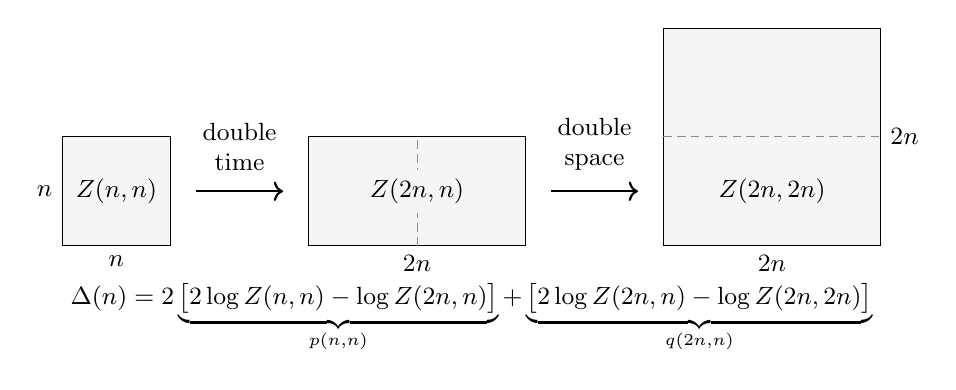
\begin{tikzpicture}[x=0.92cm,y=0.92cm,font=\small]
    \draw[fill=black!4] (0,0) rectangle (1.5,1.5);
    \node at (0.75,0.75) {$Z(n,n)$};
    \node[below] at (0.75,0) {$n$};
    \node[left] at (0,0.75) {$n$};

    \draw[->,thick] (1.85,0.75) -- (3.05,0.75);
    \node[align=center,above] at (2.45,0.9) {double\\time};

    \draw[fill=black!4] (3.4,0) rectangle (6.4,1.5);
    \draw[densely dashed,black!45] (4.9,0) -- (4.9,1.5);
    \node[fill=black!4] at (4.9,0.75) {$Z(2n,n)$};
    \node[below] at (4.9,0) {$2n$};

    \draw[->,thick] (6.75,0.75) -- (7.95,0.75);
    \node[align=center,above] at (7.35,0.9) {double\\space};

    \draw[fill=black!4] (8.3,0) rectangle (11.3,3);
    \draw[densely dashed,black!45] (8.3,1.5) -- (11.3,1.5);
    \node at (9.8,0.75) {$Z(2n,2n)$};
    \node[below] at (9.8,0) {$2n$};
    \node[right] at (11.3,1.5) {$2n$};

    \node at (5.65,-1.0)
      {$\displaystyle
        \Delta(n)=2\underbrace{\bigl[2\log Z(n,n)-\log Z(2n,n)\bigr]}_{p(n,n)}
          +\underbrace{\bigl[2\log Z(2n,n)-\log Z(2n,2n)\bigr]}_{q(2n,n)}$};
  \end{tikzpicture}\par\medskip
  \caption{The two coordinate directions enter the square-box test.
  Every rectangle has periodic boundary conditions; the dashed lines
  mark its dimensions, not cuts that make the pieces independent.
  The second doubling starts from the enlarged rectangle.
  The displayed identity is exact, with the fixed coupling suppressed.}
  \label{fig:rectangle-doubling}
\end{figure}


Define the square-box test
\begin{equation}
\label{eq:Delta}
 \Delta_\beta(n)=4\log Z_\beta(n,n)-\log Z_\beta(2n,2n).
\end{equation}
It obeys
\(\Delta_\beta(n)=2p(n,n)+q(2n,n)\ge0\). The coefficients in
\eqref{eq:Delta} cancel any term proportional to the area of the box.

\begin{samepage}
\begin{proposition}[Finite-volume criterion]
\label{prop:criterion}
Let \(n\ge4\) be even. If
\begin{equation}
 \Delta_\beta(n)\le\eta_*:=2^{-10},
\label{eq:small-test}
\end{equation}
then the transfer operators on circumferences \(2^kn\), \(k\ge0\), satisfy
\begin{equation}
 \frac{\lambda_2(2^kn)}{\lambda_1(2^kn)}
 \le e^{-(\log2)/n}.
\label{eq:width-gap}
\end{equation}
Every local limit of the square tori with sides \(2^kn\) has full gap
at least \((\log2)/n\). In particular, if the periodic infinite-plane
state is unique, then
\begin{equation}
\label{eq:criterion-gap}
 \gap(\beta)\ge\frac{\log2}{n}.
\end{equation}
\end{proposition}
\end{samepage}

\begin{proof}
Write \(\Delta=\Delta_\beta(r)\). Besides
\(q(2r,r)\le\Delta\), the definitions give
\(p(r,2r)=\Delta-2q(r,r)\le\Delta\).
Lemma~\ref{lem:squaring} therefore yields
\(p(2r,2r)\le4\Delta^2\). The rectangle identity in the other direction
gives
\[
 q(4r,r)=2q(2r,r)-2p(2r,r)+p(2r,2r)
 \le2\Delta+4\Delta^2\le3\Delta.
\]
Squaring in that direction gives \(q(4r,2r)\le36\Delta^2\). Consequently,
\begin{equation}
 \Delta_\beta(2r)
 =2p(2r,2r)+q(4r,2r)
 \le44\Delta_\beta(r)^2\le64\Delta_\beta(r)^2.
\label{eq:quadratic-recursion}
\end{equation}
Every use of the lemma is justified by \(3\eta_*<1/4\), and the smallness
condition is preserved. For \(n_k=2^kn\), induction gives
\[
 \Delta_\beta(n_k)\le\frac1{64}
          (64\eta_*)^{2^k}\le\frac1{64}2^{-2^k}.
\]
Since the first assertion of the lemma bounds
\((\lambda_2(n_k)/\lambda_1(n_k))^{n_k}\) by
\(2p(n_k,n_k)\le\Delta_\beta(n_k)\), taking the \(n_k\)-th root proves
\eqref{eq:width-gap}.

Let \(\Omega_w\) be the normalized positive ground eigenvector of
\(K_w\). For a bounded continuous observable \(F\) supported in a time slab of finite
thickness, let \(K_{w,F}\) denote the transfer kernel across that slab
with the insertion of \(F\). Pointwise,
\(|K_{w,F}|\le\norm{F}_\infty K_w^r\), where \(r\) is the number of
transfer steps across the slab. Set \(A_F=K_{w,F}/\lambda_1(w)^r\);
for \(r=0\), this is multiplication by \(F\).
Its operator norm is at most \(\norm{F}_\infty\). The infinite-time
cylinder expectation is
\(\omega_w(F)=\inner{\Omega_w}{A_F\Omega_w}\). Applying
\eqref{eq:width-gap} between two such insertions gives
\begin{equation}
 |\Cov_{\omega_w}(F,G)|\le\norm{F}_\infty\norm{G}_\infty
                           e^{-(\log2)d/n},
\label{eq:slab-bound}
\end{equation}
where \(d\) is the number of transfer edges separating their supports.
This bound passes to any local limit of the cylinder states as
\(w=2^kn\to\infty\).

We can identify these limits directly with the square-torus limits.
Let \(\widehat K_w=K_w/\lambda_1(w)\). If \(w=n_k\) and \(r\le w/2\), the
square-torus expectation is
\[
 \frac{\Tr(A_F\widehat K_w^{\,w-r})}{\Tr\widehat K_w^{\,w}}.
\]
Separating the ground projection in numerator and denominator shows that
its difference from the cylinder expectation is at most
\(2\norm{F}_\infty s_{w/2}(w)\). But
\[
 p(w/2,w)\le\Delta_\beta(w/2),\qquad
 s_{w/2}(w)\le e^{\Delta_\beta(w/2)}-1\longrightarrow0.
\]
Thus the square and cylinder expectations have the same subsequential
limits, also for products of fixed local observables. In particular,
\eqref{eq:slab-bound} holds in every such square-torus limit.

For each centered vector created by a local observable in the
reflection-positive Hilbert space, the transfer autocorrelation has a
positive spectral measure. It is a correlation of two reflected slabs,
so \eqref{eq:slab-bound} applies and excludes spectral support above
\(e^{-(\log2)/n}\) for that vector. Such vectors are dense in the vacuum
orthogonal subspace, so the same exclusion holds for the full transfer
operator. This proves \eqref{eq:criterion-gap}.
\end{proof}

The slab estimate extends to bounded measurable local observables by
approximation in their finite-dimensional distributions. No prefactor
depending on the size of a slab is needed; this will be useful for the
upper mass bound.

The criterion has reduced the problem to a single question: can one make
\(\Delta_\beta(n)\) small with \(n\) no larger than a fixed multiple of
\(\rho(\beta)^{-1}\)? The preliminary estimate alone will not do this.
It will instead supply a reference box for the comparison between cutoffs.



\section{Preliminary mixing}\label{pre:mixing}\label{pre:section}

We first prove a lattice estimate whose length scale is less precise than the
natural continuum scale, but whose uniformity under weakening bonds will be
needed later. Spins take values in the unit sphere \(S^3\subset\R^4\), identified
with the unit quaternions. The a priori measure is normalized Haar measure.
For a finite graph in the square lattice the Gibbs density is proportional to
\[
 \exp\left(\sum_{e=xy}\beta_e q_x\cdot q_y\right).
\]
Each unoriented edge occurs once. A free subgraph means that bonds outside the
graph are absent; it imposes no pinned spin values.

For a local Lipschitz observable \(F\), supported on a finite set \(A\), put
\[
 L_F=\norm{F}_\infty+\max_{x\in A}\operatorname{Lip}_x(F),
\]
where the individual Lipschitz constant uses round distance on \(S^3\) with
all other spins fixed. Distances between supports use the maximum norm, or
its periodic version on a torus.

\begin{theorem}[Preliminary mixing]\label{thm:preliminary}
There are fixed positive constants \(C,c,p\) such that, on setting
\begin{equation}
 \Xi(\beta)=\exp\left[\pi\beta+
 C\sqrt{(1+\beta)\log(2+\beta)}\right],
 \label{eq:pre:Xi}
\end{equation}
the following hold for every \(\beta\geq0\).

For every unpinned rectangular torus with each side at least \(C\Xi(\beta)\),
and every choice \(0\leq\beta_e\leq\beta\), local observables \(F,G\) supported
on \(A,A'\) at distance \(d\) satisfy
\begin{equation}
 |\Cov(F,G)|\leq C(1+\beta+|A|+|A'|+d)^{20}
 L_FL_G e^{-cd/\Xi(\beta)}.
 \label{eq:pre:theorem-mixing}
\end{equation}
The same bound holds on every unpinned free subgraph, with ambient lattice
distance. In the homogeneous model the local limit of periodic square
measures is unique.

Let \(Z_\beta(n,m)\) be the partition function of the homogeneous
\(n\)-by-\(m\) torus. For every even \(n\geq C\Xi(\beta)\),
\begin{equation}
 0\leq\Delta_\beta(n):=4\log Z_\beta(n,n)-\log Z_\beta(2n,2n)
 \leq C(1+\beta)^pn^p e^{-cn/\Xi(\beta)}.
 \label{eq:pre:theorem-delta}
\end{equation}
\end{theorem}

The proof first obtains a small stiffness on a suitable pinned square. This
part allows arbitrary signed couplings and fixed right twists. We then use
coarse orientation variables to prove decay for charged observables. Two
conditional decompositions into ferromagnetic circle and Ising systems give
mixing for arbitrary local observables. Only this last part requires
nonnegative untwisted couplings.

Constants denoted by \(C\) may increase from line to line. All are independent
of lattice size and of the particular couplings and pins. Dependence on a
fixed moment order or a fixed auxiliary exponent is indicated when needed.
For continuum test fields on the unit square, \(\|\cdot\|_2\) denotes the
Lebesgue \(L^2\) norm. For random variables, \(\|\cdot\|_p\) denotes the
probabilistic \(L^p\) norm.

\subsection{Local class and Ward identities}\label{pre:local}

The following calculation is a local Ward identity, in the tradition of
\cite{Mermin1967,DriesslerLandauPerez,AizenmanSimonWard}. We give the full
quaternion formula because the noncommuting current term and its factor
two determine the quantitative stiffness gain.

Work on \(Q(S)=\{0,\ldots,S\}^2\) with all boundary spins fixed. For each positively oriented edge \(e=x\to y\), set

\[
 t_e+s_e=q_yU_eq_x^{-1},\qquad t_e\in\mathbb R,\quad s_e\in\operatorname{Im}\mathbb H\simeq\mathbb R^3,
\]

where \(U_e\) is any fixed unit quaternion. Take signed coefficients \(|b_e|\leq b\leq B\), with \(w_e=b_e\) except that edges tangent to the boundary carry \(w_e=b_e/2\). The local density is \(Z^{-1}\exp(\sum_e w_et_e)\). The half allocation makes adjacent cell actions sum exactly to the action on the union.

For macroscopic midpoint coordinates \(z_e\), define

\[
 X_Q(F)=S^{-1}\sum_e w_es_e\cdot F_{\mu(e)}(z_e),
\]

\begin{equation}
 \mathcal H_Q(F,G)=S^{-2}\mathbb E\sum_e w_et_e\,\overline{F_e}\cdot G_e
 -\operatorname{Cov}(X_Q(F),X_Q(G)).
\label{eq:pre:1-1}
\end{equation}

The covariance is sesquilinear, with conjugation on the first entry. Write \(H_Q\) for the restriction to constant \(3\times2\) matrices. In each spatial direction the sum of the absolute edge coefficients is at most \(bS^2\): there are \(S(S-1)\) interior edges and two tangent boundary rows with half weight. Thus

\begin{equation}
H_Q\leq bI.
\label{eq:pre:1-2}
\end{equation}

This is valid with signed coefficients and twists. No positive lower bound on \(H_Q\) is claimed or used.

For an imaginary unit \(a\), rotate \(q_x\mapsto e^{af_x}q_x\). A bond quaternion changes to \(e^{af_y}(t_e+s_e)e^{-af_x}\). Its \((1,a)\)-plane rotates through \(f_y-f_x\); its imaginary plane perpendicular to \(a\) rotates through \(f_y+f_x\). If \(\mathcal A=-\sum w_et_e\), then

\begin{equation}
 D_f\mathcal A=\sum_e w_e(s_e\cdot a)(f_y-f_x),\qquad
 D_f^2\mathcal A=\sum_e w_et_e(f_y-f_x)^2.
\label{eq:pre:1-3}
\end{equation}

For a general infinitesimal imaginary profile \(\eta_x\), the imaginary bond derivative is exactly

\begin{equation}
D_\eta s_e=t_e(\eta_y-\eta_x)+(\eta_y+\eta_x)\times s_e.
\label{eq:pre:1-4}
\end{equation}

Consequently the compact-profile Ward identity has a contact term and a bracket term. If \(\eta\) vanishes on the fixed boundary, Haar integration by parts gives

\begin{equation}
\mathbb E[\overline{X_Q(d_S\eta)}X_Q(F)]
=S^{-2}\mathbb E\sum_e w_et_e\overline{(d_S\eta)_e}\cdot F_e
+\mathbb E X_Q\!\left(F_e\times(\overline{\eta_y}+\overline{\eta_x})\right),
\label{eq:pre:1-5}
\end{equation}

where the cross product is extended complex bilinearly. This follows first
for real profiles and then by complex linear extension. Here
\((d_S\eta)_\mu(z)=S[\eta(z+e_\mu/(2S))-\eta(z-e_\mu/(2S))]\).
This fixes the normalization and the factor two in the eventual nonabelian derivative. For the same-axis score there is no bracket term; \eqref{eq:pre:1-3} follows directly.


\subsection{Current moments near a pinned boundary}\label{pre:moments}

Assume throughout the local induction

\begin{equation}
\log(2+S)\leq16B.
\label{eq:pre:2-1}
\end{equation}

\begin{lemma}[Uniform current moments]\label{pre:current-moments}
For every fixed \(1\leq p<\infty\),

\begin{equation}
\|X_Q(F)\|_p\leq C_p(1+b)\log(2+S)\|F\|_{C^1}.
\label{eq:pre:2-2}
\end{equation}

Here and subsequently the derivative norm is in the indicated rescaled coordinates. The constants are independent of pins, signs, twists, and side length.
\end{lemma}

\begin{proof}

\subsubsection{Compact scores}\label{pre:part-2-1}

For a real one-axis profile \(f\) zero at the pinned boundary, the second variation along the full rotation path is bounded in absolute value by
\(b\sum_e(f_y-f_x)^2\). Taylor's formula and invariance of the Haar integral under the compact rotation imply

\begin{equation}
\mathbb E\exp(tD_f\mathcal A)
\leq\exp\left[\tfrac12 b t^2\sum_e(f_y-f_x)^2\right].
\label{eq:pre:2-3}
\end{equation}

Here \(E(f)=\sum_e(f_y-f_x)^2\) and \(q^{tf}_x=e^{atf_x}q_x\).
Use \(\mathcal A(q^{-tf})\leq\mathcal A(q)-tD_f\mathcal A(q)+\frac12bt^2E(f)\), exponentiate, and integrate. The same Taylor estimate bounds the \(r\)-th moment of the likelihood ratio of a unit rotation by \(\exp(C_r bE(f))\). It is therefore bounded when \(bE(f)\) is bounded. These arguments use \(|w_et_e|\leq b\), so remain valid for signed and twisted interactions.

\subsubsection{Extracting a transverse current on a buffered patch}\label{pre:part-2-2}

Take an interior patch of lattice side \(d\), with a proportional buffer. For a scalar test \(h\) on the inner patch, let \(H\) be its \(C^1\) norm in patch coordinates. Choose a compact scalar potential \(\vartheta\), affine with slope \(1/d\) in direction \(\mu\) on all edges meeting the support of \(h\), and with bounded Dirichlet energy. Choose \(a\) perpendicular to the current color to be extracted. The compact score in the other perpendicular color has every fixed moment \(O_p(\sqrt b)\) by \eqref{eq:pre:2-3}.

Assume \(H>0\), since otherwise the test is zero. Rotate this score by the two opposite profiles

\[
 f=\tfrac12\arcsin(h/N),\qquad N=C\sqrt{1+b}\,H.
\]

The rotations have uniformly bounded likelihood norms. The difference of the rotated scores is the transverse current multiplied by \(2\sin(f_x+f_y)\). Multiplication by \(N\) extracts \(h\) at the midpoint up to \(CH/d\). It is important that only this first-order error is needed: after the score normalization \(d^{-1}\), its deterministic total over \(O(d^2)\) edges is \(O(bH)\). The moment cost of the two scores multiplied by \(N\) is \(O_p((1+b)H)\). Hence

\begin{equation}
\left\|d^{-1}\sum_{e\parallel\mu}w_e(s_e)_k h_e\right\|_p
\leq C_p(1+b)H.
\label{eq:pre:2-4}
\end{equation}

Bounded \(d\) can be treated deterministically.

\subsubsection{Whitney summation}\label{pre:part-2-3}

A width \(O(1)\) boundary layer contributes \(O(b\|F\|_\infty)\). Decompose the remaining square into buffered patches with \(d\) comparable to distance to the boundary. At one dyadic scale there are \(O(S/d)\) such patches; their normalized tests have \(C^1\) norms \(O(\|F\|_{C^1})\). Applying \eqref{eq:pre:2-4}, multiplying by \(d/S\), and summing gives \(O((1+b)\|F\|_{C^1})\) per scale. There are \(O(\log(2+S))\) scales. This proves \eqref{eq:pre:2-2}.
\end{proof}


\subsection{Conditioning into cells}\label{pre:cells}

The symbol \(L\) in this preliminary argument is an auxiliary integer
which may change during the stiffness iteration. It is independent of
the fixed block size chosen for the exact renormalization map in
Section~\ref{free:section}.

The current-moment estimate permits replacing slowly varying fields by
their values at cell anchors. We next express the large-square stiffness
through the conditioned cell laws; the variance of their conditional
currents is the gain to exploit.

Tile \(Q(S)\) by \(L^2\) cells of side \(R=S/L\). Condition on their complete boundary rings \(\omega\). Cell interiors are independent and the ring density has action
\(S_g(\omega)=-\sum_c\log Z_c(\omega)\). Set

\[
j(F)=\mathbb E[X_Q(F)\mid\omega]
=L^{-1}\sum_c\mathbb E_cX_c(F).
\]

Let \(z_c\) be the lower-left cell anchor and put

\[
N_c(F)=\sup_{c^+}(|F|+L^{-1}|\nabla F|),\qquad
D_c(F)=L^{-1}N_c(\nabla F).
\]

The fixed enlargement \(c^+\) is used only for smooth test-field estimates. Write \(P(B)\) for a fixed polynomial whose degree and coefficients may depend on fixed moment orders or prescribed exponents, but not on \(R,L,S\). Equation \eqref{eq:pre:2-2} and \eqref{eq:pre:2-1} give

\begin{equation}
|\mathbb E_cX_c(F)|\leq P(B)N_c(F),\quad
|\mathcal H_c(F,G)|\leq P(B)N_c(F)N_c(G),
\label{eq:pre:3-1}
\end{equation}

\begin{equation}
|\mathcal H_c(F,G)-\overline{F_c}H_cG_c|
\leq P(B)[D_c(F)N_c(G)+N_c(F)D_c(G)].
\label{eq:pre:3-2}
\end{equation}

For the last estimate subtract the constants \(F_c,G_c\) in the bilinear form. Their remainders have cell-coordinate \(C^1\) norm bounded by the displayed \(D_c\). One can instead use a direct Lipschitz bound on the cell where appropriate.

For a scalar ring rotation \(u\), let \(H_c^u\) be the resulting constant-field stiffness and \(O_c(u)=\operatorname{Ad}(e^{au(z_c)})\). Then

\begin{equation}
\|O_c(u)^TH_c^uO_c(u)-H_c\|\leq P(B)D_c(u),
\label{eq:pre:3-3}
\end{equation}

and its derivative at zero satisfies the same bound. To prove this, remove the constant rotation \(u(z_c)\) exactly by covariance. Along the remaining path also rotate the interior integration variables. The logarithmic density derivative is the negative of the centered cell current with test \(aR(u_y-u_x)\), whose fixed moments are bounded by \(P(B)D_c(u)\). The residual profile need not vanish on the cell boundary; the current-moment bound applies to this test without that restriction. Derivatives of a constant-field current have the bracket current with residual profile of size \(D_c(u)\), plus a deterministic contact of that size. Differentiate the contact and covariance in \eqref{eq:pre:1-1} and apply H\"older with the already established current moments. Restarting this calculation at each point of the path gives the bound for arbitrary amplitude \(u\); there is no exponential dependence on its constant part.

Rotating all rings while fixing the outside boundary gives the exact Hessian identity

\begin{equation}
D_u^2S_g=L^{-2}\sum_c\mathcal H_c(a\,d_Su,a\,d_Su).
\label{eq:pre:3-4}
\end{equation}


\subsection{Gaussian augmentation and commuting derivatives}\label{pre:gaussian}

The cell stiffness matrices need not be positive. We add auxiliary
Gaussian noise so that the desired upper bound on $H_Q$ becomes a lower
bound on the variance of an augmented current. The identity below makes
this reduction exact.

Suppose uniformly throughout the pinned cell class
\(H_c\leq hI\), where \(B^{-D}\leq h\leq B\). Choose

\begin{equation}
h<v\leq2B,\qquad c_0\geq B^{-D'},\qquad
C_c=vI-H_c-c_0P_a\geq B^{-D'}I,
\label{eq:pre:4-1}
\end{equation}

where \(P_a\) is projection onto the two spatial components of color \(a\). Let \(n_c\) be independent standard six-dimensional Gaussian vectors, and \(n_{0,c}\) independent two-dimensional Gaussian vectors of covariance \(c_0I\), all independent of the true ring data. Define

\begin{equation}
J(F)=j(F)+L^{-1}\sum_c(\sqrt{C_c}n_c+a n_{0,c})\cdot F_c.
\label{eq:pre:4-2}
\end{equation}

For every constant real matrix \(A\), total variance gives exactly

\begin{equation}
H_Q(A,A)=v|A|^2-\operatorname{Var}J(A).
\label{eq:pre:4-3}
\end{equation}

Indeed \(H_Q=L^{-2}\sum_c\mathbb EH_c-\operatorname{Var}j\), and the conditional noise covariance adds \(vI-L^{-2}\sum_cH_c\).

Choose a real trigonometric cutoff \(\psi\), zero on the boundary, with band \(O(m)\). Let \(f_i=\psi\varphi_i\), where \(\varphi_i\) are the real orthonormal Fourier modes of frequency \(|k|\leq4K\), including the constant. Use \(K+m\ll L\) and

\[
G_0=L^{-2}\sum_c\nabla f(z_c)\nabla f(z_c)^T,
\quad
p=(c_0G_0)^{-1}L^{-1}\sum_c\nabla f(z_c)n_{0,c},
\quad \theta=f\cdot p.
\]

Quadrature is exact at this band, so \(G_0\) is the continuum gradient Gram matrix. It is positive: a linear combination of the \(f_i\) with zero gradient is a constant, zero on the boundary, and hence is zero; division by \(\psi\) on its open nonzero set then annihilates the Fourier polynomial. Thus \(p\) is Gaussian with covariance \((c_0G_0)^{-1}\).

Put

\[
\omega^0=e^{-a\theta}\omega,\qquad
n_{0,c}^0=n_{0,c}-c_0\nabla\theta(z_c)/L,
\]

\[
n_c^0=O_c(\theta)^Tn_c-\sqrt{C_c^0}\,a\nabla\theta(z_c)/L,
\]

where \(C_c^0\) uses \(\omega^0\). At fixed base data \((\omega^0,n_0^0,n^0)\), the density of \(p\) is proportional to \(e^{-V(p)}\), with

\begin{equation}
V(p)=\tfrac12c_0p^TG_0p+S_g(e^{a\theta}\omega^0)
+\tfrac12\sum_c|n_c^0+\sqrt{C_c^0}\,a\nabla\theta(z_c)/L|^2.
\label{eq:pre:4-4}
\end{equation}

This is an exact change of variables. First split the Gaussian \(n_0\) into its linear projection and orthogonal residual. At fixed \(p\), the ring rotation preserves product Haar measure. At fixed \(p,\omega^0\), the \(n_c\) transformations are orthogonal maps followed by translations. These successive maps have constant Jacobian; dependencies of later maps on earlier variables give a triangular Jacobian, not an extra determinant.

For fixed scalar directions \(u_i\) in the potential span, let \(\partial_i\) mean addition of \(tu_i\) to \(\theta\) with all base data fixed. They commute. Conditional integration by parts gives, for \(\partial_i^*=-\partial_i+\partial_iV\),

\begin{equation}
\mathbb E\left(\sum_i\partial_i^*Y_i\right)^2
=\mathbb E\sum_{ij}(\partial_jY_i)(\partial_iY_j)
+\mathbb E\sum_{ij}Y_i(\partial_i\partial_jV)Y_j.
\label{eq:pre:4-5}
\end{equation}

The identity first holds conditionally and then in the full law. The conditional density has Gaussian decay: its first term is strictly positive quadratic and \(S_g\) is bounded for each fixed finite system. The functions involved and their derivatives have at most polynomial growth in Gaussian variables, since the matrices remain in a fixed positive cone for that system. Thus the integration by parts has no missing boundary term.


\subsection{Three uniform band estimates}\label{pre:bands}

The integration-by-parts identity in the preceding subsection contains
a Hessian term and a crossed derivative term. We next control their
ingredients uniformly in the number of modes, while retaining the exact
contact cancellation in the Ward identity.

Fix \(D,D'\) and any requested power \(N\). Take \(K/L\leq B^{-J}\), with \(J\) sufficiently large depending only on these fixed numbers and on the fixed test amplitude bounds. Retain \(S\geq L\), \eqref{eq:pre:2-1}, and \(Bm\leq K\). The constants denoted \(P(B)\) below do not depend on the subsequently increased \(J\).

\subsubsection{Sampling, gradients, and the good event}\label{pre:part-5-1}

For any trigonometric field of band \(O(K)\), with \(K\ll L\), we have

\begin{equation}
\|N(F)\|_\square\leq C\|F\|_2,\qquad
\|D(F)\|_\square\leq C(K/L)\|F\|_2,
\quad
\|a\|_\square^2=L^{-2}\sum_c|a_c|^2.
\label{eq:pre:5-1}
\end{equation}

Here is a direct sampling proof. Choose a smooth frequency cutoff equal to
one on the allowed band and supported in a ball of radius \(cL\), with fixed
\(c\). Its periodic convolution kernel \(K_L\) satisfies, for any fixed
\(N_0>2\),
\[
 |\partial^r K_L(z)|\leq C_{r,N_0}L^{2+r}
 (1+L\operatorname{dist}(z,\mathbb Z^2))^{-N_0}.
\]
This follows by writing the kernel as the periodization of the rescaled
inverse Fourier transform of the smooth cutoff and integrating that
transform by parts. Since \(F=K_L*F\), weighted Cauchy gives
\[
 \sup_{z\in c^+}|F(z)|^2\leq
 CL^2\int (1+L\operatorname{dist}(z_c-y,\mathbb Z^2))^{-N_0}|F(y)|^2\,dy.
\]
Sum over cells and divide by \(L^2\); the remaining lattice sum is bounded.
Apply the same argument to derivatives and use Parseval,
\(\|\partial^rF\|_2\leq(CK)^r\|F\|_2\). This proves
\eqref{eq:pre:5-1}, including its constant independent of the number of cells.
The centered-difference Fourier multiplier also gives

\begin{equation}
\|d_Su-\nabla u\|_2\leq C(K/S)^2\|\nabla u\|_2.
\label{eq:pre:5-2}
\end{equation}

Although the matrix \(G_0\) need not be well conditioned in the chosen basis, that is immaterial. The covariance of \(\nabla\theta\) is \(c_0^{-1}\) times the orthogonal projection onto the gradient subspace. Evaluation of a band \(O(K)\) gradient field has norm at most \(CK\), and evaluation after one more derivative at most \(CK^2\). Therefore

\begin{equation}
\rho=L^{-1}\|\nabla\theta\|_\infty+L^{-2}\|\nabla^2\theta\|_\infty
\leq B^{-n}
\label{eq:pre:5-3}
\end{equation}

outside an event of probability at most \(e^{-B^3}\), for any prescribed fixed \(n\) if \(J\) is large enough. For the supremum bound one can use only the elementary Fourier estimate
\(\|\nabla F\|_\infty\leq CK^2\|F\|_2\leq CK^2\|F\|_\infty\)
on this unit-volume torus. A grid of spacing \(cK^{-2}\) therefore captures
at least half the supremum. It has \(O(K^4)\leq e^{CB}\) points by
\eqref{eq:pre:2-1}. At each point the gradient standard deviation is at most
\(CK/\sqrt{c_0}\), and that of one more derivative at most
\(CK^2/\sqrt{c_0}\). After division by \(L\) and \(L^2\), respectively,
the Gaussian tail exponent at the threshold in \eqref{eq:pre:5-3} is an
arbitrarily high fixed power of \(B\) when \(J\) is increased. This proves
the claimed probability after the finite union bound.

\subsubsection{Hessian estimate}\label{pre:part-5-2}

From \eqref{eq:pre:4-4} and \eqref{eq:pre:3-4}, the exact conditional Hessian is the sum of the cell stiffness form and the two quadratic noise forms. Replace \(d_Su\) by \(\nabla u(z_c)\) using \eqref{eq:pre:3-2}, \eqref{eq:pre:5-1}, and \eqref{eq:pre:5-2}. Conjugate each true cell stiffness back to its base value using \eqref{eq:pre:3-3}. The color \(a\) is fixed by \(O_c\). The total error on \eqref{eq:pre:5-3} is at most

\[
P(B)[K/L+(K/S)^2+\rho]\,\|\nabla u\|_2^2.
\]

The remaining matrix sum is exactly \(H_c^0+C_c^0+c_0P_a=vI\). Consequently, for all directions simultaneously,

\begin{equation}
\partial_u^2V\leq(v+B^{-N})\|\nabla u\|_2^2
\label{eq:pre:5-4}
\end{equation}

on the good event. Everywhere the same upper bound holds with \(P(B)\) in place of \(v+B^{-N}\), by \eqref{eq:pre:3-1}, \eqref{eq:pre:4-1}, and \eqref{eq:pre:5-1}. The crude bound

\begin{equation}
\|J(F)\|_p\leq C_pP(B)L\|F\|_2
\label{eq:pre:5-5}
\end{equation}

follows from \eqref{eq:pre:3-1}, Cauchy over cells, and conditional Gaussian moments. Thus an exceptional event of probability \(e^{-B^3}\) contributes an arbitrary inverse power of \(B\) to every later finite moment expression, even if that expression has a fixed polynomial number of modes and a fixed polynomial factor in \(L\): \(\log L\leq16B\).

\subsubsection{Nonabelian derivative estimate}\label{pre:part-5-3}

Let at most \(CK^2\) real directions \(u_i\) satisfy

\begin{equation}
\|\nabla\sum_i d_i u_i\|_2\leq C|d|,\qquad
N_c(\nabla u_i)\leq C.
\label{eq:pre:5-6}
\end{equation}

For real deterministic \(F\) of band \(O(K)\), perpendicular in color to \(a\), write \(F'=-a\times F\). Then

\begin{equation}
\mathbb E\sum_i|\partial_iJ(F)-2J(u_iF')|^2
\leq B^{-N}\|F\|_2^2.
\label{eq:pre:5-7}
\end{equation}

Here is the termwise proof. For \(u=\sum d_iu_i\), differentiation of the physical conditional mean gives exactly

\begin{equation}
\partial_u j(F)=2j(uF')+j(r_uF')
+L^{-2}\sum_c\mathcal H_c(a\,d_Su,F),
\label{eq:pre:5-8}
\end{equation}

where \((r_u)_\mu(z)=u(z+e_\mu/(2S))+u(z-e_\mu/(2S))-2u(z)\). Taylor or Fourier multipliers give
\(\|r_u\|_2\leq CK S^{-2}\|\nabla u\|_2\).
Using cell products in \eqref{eq:pre:3-1} and \eqref{eq:pre:5-1},

\begin{equation}
|j(r_uF')|\leq P(B)LK S^{-2}\|\nabla u\|_2\|F\|_2.
\label{eq:pre:5-9}
\end{equation}

The anchor-conjugation part of differentiating \(\sqrt{C_c}\) combines with the derivative of \(n_c=O_c(\theta)(n_c^0+\sqrt{C_c^0}a\nabla\theta/L)\) to give exactly the noise part of \(2J(uF')\). The \(n_0\) noise is in color \(a\) and pairs to zero. The remaining deterministic noise drift is

\begin{equation}
L^{-2}\sum_c F_c\cdot\sqrt{C_c}\,O_c(\theta)\sqrt{C_c^0}\,a\nabla u(z_c).
\label{eq:pre:5-10}
\end{equation}

On the good event, \eqref{eq:pre:3-3} and the positive lower bound in \eqref{eq:pre:4-1} imply
\(\sqrt{C_c}O_c\sqrt{C_c^0}a=C_ca+O(P(B)\rho)\).
Together with the anchored version of the last term in \eqref{eq:pre:5-8}, this leaves \(F_c\cdot(H_c+C_c)a\nabla u\), which is zero because \(H_c+C_c=vI-c_0P_a\) and \(F\perp a\). The error is at most

\begin{equation}
P(B)[K/L+(K/S)^2+\rho]\|\nabla u\|_2\|F\|_2.
\label{eq:pre:5-11}
\end{equation}

Both \eqref{eq:pre:5-9} and \eqref{eq:pre:5-11} are bounds on a \emph{real scalar linear functional of \(d\)}, holding pointwise uniformly for \(|d|\leq1\). Its squared norm is precisely the sum of the squared errors in the individual directions. One must not multiply these bounds by the number of directions. Complex test fields follow by applying the estimate separately to their real and imaginary parts, at the cost of a fixed factor.

There remains the non-anchor square-root derivative \(\Gamma_c(u_i)\), with
\(\|\Gamma_c(u_i)\|\leq P(B)L^{-1}N_c(\nabla u_i)\).
At the true data the corresponding error is
\(L^{-1}\sum_cF_c\cdot\Gamma_c(u_i)n_c\).
The noises \(n_c\) are independent of \(\omega,p\); \(\Gamma_c(u_i)\) depends on \(\omega\) and the deterministic direction, not on these noises. Hence

\begin{equation}
\sum_i\mathbb E\left|L^{-1}\sum_cF_c\cdot\Gamma_c(u_i)n_c\right|^2
\leq P(B)\frac{K^2}{L^2}\|F\|_2^2.
\label{eq:pre:5-12}
\end{equation}

This last estimate does count the \(O(K^2)\) directions; its smallness comes from \(K/L\). On the exceptional angular event use the everywhere polynomial drift bound, and then its probability. Equations \eqref{eq:pre:5-9}--\eqref{eq:pre:5-12} prove \eqref{eq:pre:5-7} after choosing \(J\) sufficiently large. They explain exactly where a dimension loss is and is not allowed.

\subsubsection{Same-frequency Ward bound}\label{pre:part-5-4}

For the uncentered defect

\[
\mathcal D(F,G)=vL^{-2}\sum_c\overline{F_c}\cdot G_c
-\mathbb E\overline{J(F)}J(G),
\]

total covariance splitting and \eqref{eq:pre:3-2} compare it to the raw defect from \eqref{eq:pre:1-5}, with error

\begin{equation}
P(B)(K/L)\|F\|_2\|G\|_2.
\label{eq:pre:5-13}
\end{equation}

Let \(\eta=r\xi(z)e^{ik\cdot z}/(i|k|)\), with \(\eta\) zero on the boundary, \(|r|\leq1\), \(m\leq|k|\leq CK\), and \(\xi\) having band \(O(m)\), bounded supremum, and fixed polynomial \(C^3\) bounds. Let \(G\) be an exact gradient of a potential of the same type and frequency, or a bounded constant matrix times \(\xi_2e^{ik\cdot z}\). Require the amplitude's first derivative divided by \(|k|\) bounded, as is the case in all uses below. Apply \eqref{eq:pre:1-5} with \(\eta\) as defined; the identity already conjugates its first argument. Its contact cancels the raw defect. In the bracket term the two Fourier phases cancel even at the centered endpoints; the remaining current test has \(C^1\) norm \(P(B)/|k|\). For a gradient \(G\), its centered amplitude differences and the factors \(S\sin(k_\mu/(2S))\) have the same bound after division by \(|k|\). Thus \eqref{eq:pre:2-2} and \eqref{eq:pre:5-13} imply

\begin{equation}
|\mathcal D(d_S\eta,G)|\leq P(B)/|k|+B^{-N}.
\label{eq:pre:5-14}
\end{equation}

The raw Ward identity must be applied before replacing the gradient by its leading Fourier symbol. Otherwise the exact contact cancellation is lost.


\subsection{A weighted current estimate}\label{pre:weighted}

The band estimates control differentiated currents. We now sum them with
frequency weights whose convolutions remain summable. This is the
auxiliary estimate needed to bound the crossed derivative term in the
variance gain; it is not yet the stiffness improvement itself.

Fix an integer \(N_*>100(1+D+D')\) and apply the band estimates with accuracy
\(B^{-10N_*}\). Increase the fixed exponent \(J\) whenever required below.
The error estimates in the next two subsections are then bounded by
\(C B^{-N_*}\). To track this convention, all remaining weighted frequency
sums are bounded by fixed powers of \(T,T_w\leq CB\); all cutoff derivative
and cell-moment constants are fixed powers of \(B\). The only crude factors
in \(L\) occur with an \(S^{-2}\) Taylor remainder or an event of probability
\(e^{-B^3}\). Since \(S\geq L\) and \(\log L\leq16B\), those errors are
also at most \(B^{-N_*}\). No unweighted count of the main frequency band
is used in this convention.

Choose a sufficiently large fixed exponent \(J\) and set

\[
M=B^J,\quad K=L/B^J,\quad L\geq B^{10J},
\quad
\psi(z)=\prod_{\mu=1}^2[1-\cos^{2m}(\pi z_\mu)],
\quad m=\lceil B^4\rceil.
\]

All fixed powers of \(\psi\) have Fourier \(\ell^1\) norm bounded independently of \(B\), band \(O(m)\), and fixed derivative bounds polynomial in \(B\). Put \(\chi=\psi^2\); then

\begin{equation}
I_\chi=\int_{[0,1]^2}\chi^2\geq1-CB^{-2}.
\label{eq:pre:6-1}
\end{equation}

This follows from the Gaussian decay of \(\cos^{2m}(\pi z)\) away from the seams and an exceptional width \(O(m^{-1/2})\).

In a long step use \(K_1=L/B^{4J}\), \(K_2=L/B^{3J}\). In a short step use \(K_1=8M\), \(K_2=256M\). The main reciprocal lattice is \(2\pi\mathbb Z^2\), and

\begin{equation}
T=\sum_{M\leq|k|\leq K_1}|k|^{-2}
=\frac1{2\pi}\log(K_1/M)+O(M^{-1}),\qquad c\leq T\leq CB.
\label{eq:pre:6-2}
\end{equation}

The coefficient is \((2\pi)^{-2}\times2\pi=1/(2\pi)\). The sum here includes both signs of the Fourier frequencies, equivalently both normalized real modes for each pair.

\subsubsection{The weight and its convolution}\label{pre:part-6-1}

For dyadic \(H\) from \(M\) up to \(K_2\), let

\[
p_H(k)=H^{-2}e^{-\sqrt{|k|/H}},\quad
w(k)=\sum_Hp_H(k),\quad T_w=\sum_kw(k).
\]

Then

\begin{equation}
T_w\asymp1+\log(K_2/M),\quad
w*w\leq CT_ww,\quad
(m+|k|)^2w(k)\leq C,
\label{eq:pre:6-3}
\end{equation}

and \(w(k)\geq c(M+|k|)^{-2}\) for \(|k|\leq K_2/2\). Shifts of size \(O(m)\) change \(w\) by at most a fixed factor.

For completeness, if \(H\leq H'/4\),

\[
\sqrt{|l|/H}+\sqrt{|k-l|/H'}
\geq\tfrac12\sqrt{|l|/H}+\sqrt{|k|/H'},
\]

so summing \(l\) proves \(p_H*p_{H'}\leq Cp_{H'}\). If \(H'/4\leq H\leq H'\), split into \(|l|\leq|k-l|\) and its complement and use

\[
\sqrt{|l|}+\sqrt{|k-l|}\geq\sqrt{|k|}+c\sqrt{\min(|l|,|k-l|)}.
\]

The retained exponential is summable on the comparable scale. Summing over the dyadic pair of scales proves the convolution bound. The other claims follow directly by dyadic summation.

The tail \(|k|>K-O(m)\) is negligible to every fixed inverse power of \(B\), even against fixed polynomial factors in \(L,B,|k|/L\). In the long case \(\sqrt{K/K_2}=B^J\), whereas \(\log L\leq16B\); the short case has an even larger separation.

\subsubsection{Closing a two-color estimate}\label{pre:part-6-2}

Fix perpendicular colors \(r,r'\), with \(r'=-a\times r\). For both real modes in each frequency pair with \(2M\leq|k_p|\leq4M\), put

\[
b_p=|k_p|^{-2},\qquad
G_p^r=r\,d_S(\psi\widetilde\varphi_p/|k_p|),
\]

where the quadrature modes are \(\sqrt2\sin,-\sqrt2\cos\) for \(\sqrt2\cos,\sqrt2\sin\), respectively. The Ward bound gives

\begin{equation}
\sum_pb_p\mathbb E J(G_p^r)^2\leq Cv.
\label{eq:pre:6-4}
\end{equation}

Indeed the summed contact is \(O(v)\), the annular sum of \(b_p\) is \(O(1)\), and the error \(P(B)/M+B^{-N}\) can be made \(o(v)\).

Take directions \(u_i=\sqrt{w(k_i)}\psi\varphi_i\), \(|k_i|\leq K\), and set

\[
Y_{pi}=J(G_p^ru_i),\qquad
U^r=\sum_pb_p\sum_i\mathbb E Y_{pi}^2.
\]

The directions obey \eqref{eq:pre:5-6} by \eqref{eq:pre:6-3}, Parseval,
and the bounded multiplier norms of \(\psi\). Use the adjoints for the
base-data-fixed conditional law in \eqref{eq:pre:4-5}, and define
\[
 D_p=\sum_i\partial_i^*Y_{pi},\qquad F_p=-G_p^{r'}.
\]
The sign is fixed by \((r')'=-r\): the prime field of \(F_p\) is
\(G_p^r\). Conditional integration by parts and
\eqref{eq:pre:5-7} therefore give
\[
 \sum_pb_p\mathbb E[J(F_p)D_p]
 =\sum_{pi}b_p\mathbb E[(\partial_iJ(F_p))Y_{pi}]
 =2U^r+O(B^{-N_*})\sqrt{U^r}.
\]
Weighted Cauchy and \eqref{eq:pre:6-4} bound the square of this expression
by \(Cv\sum_pb_p\mathbb ED_p^2\). To estimate the latter sum, apply
\eqref{eq:pre:4-5} to each vector \(Y_p\). The Hessian contribution is
at most \(CvU^r+O(B^{-N_*})\). Bound the crossed derivative term by
\(\sum_{pij}b_p\mathbb E|\partial_jY_{pi}|^2\). A second use of
\eqref{eq:pre:5-7} bounds this Frobenius sum by

\begin{equation}
C\sum_{pij}b_p\mathbb E|J(G_p^{r'}u_iu_j)|^2+O(B^{-N_*})
\leq CT_wU^{r'}+O(B^{-N_*}).
\label{eq:pre:6-5}
\end{equation}

For the last inequality use complex Fourier modes in \(i,j\), apply \(w*w\leq CT_ww\), and remove the extra power of \(\psi\) by its bounded Fourier \(\ell^1\) norm and the shift bound for \(w\). Frequencies beyond the truncated set are negligible by the preceding tail estimate and the elementary extension of \eqref{eq:pre:5-5}, \(\|J(G_p^{r'}\psi e^{ikz})\|_2\leq P(B)L(1+|k|/L)\). The derivative-error sum costs \(B^{-N}\sum_i\|G_p^ru_i\|_2^2\leq CB^{-N}T_w\), not \(B^{-N}K^2\).

We have consequently proved
\[
 \sum_pb_p\mathbb ED_p^2
 \leq CvU^r+CT_wU^{r'}+O(B^{-N_*}).
\]
Interchanging the colors gives the same inequality with \(r,r'\)
reversed, since \(U^{-r}=U^r\).
Thus neither color estimate is assumed in proving the other.
Let \(U=\max(U^r,U^{r'})\). Unless \(U\leq CB^{-2N_*}\), the signal lower
bound gives
\(U^2\leq Cv(v+T_w)U+CvB^{-N_*}\).
Solving this quadratic and using \(v\geq B^{-D}\) gives

\begin{equation}
U^r+U^{r'}\leq Cv(v+T_w).
\label{eq:pre:6-6}
\end{equation}

\subsubsection{Extracting all spatial directions}\label{pre:part-6-3}

At fixed total complex frequency \(n=k_p+k_i\), \(|n|\leq4K_1\), take the common positive lower bound
\(w(n-k_p)\geq c(M+|n|)^{-2}\). Write
\[
 \psi_\mu^+(z)=\frac12\bigl[\psi(z+e_\mu/(2S))+
                         \psi(z-e_\mu/(2S))\bigr].
\]
The exact gradient factor in spatial direction \(\mu\) is

\[
\widehat k_{p\mu}\operatorname{sinc}(k_{p\mu}/(2S))\psi_\mu^+
+\frac{S\cos(k_{p\mu}/(2S))}{i|k_p|}
[\psi(z+e_\mu/(2S))-\psi(z-e_\mu/(2S))].
\]

Under \(k_p\mapsto-k_p\) its first part changes sign and its second part does not. Pairing the two squared currents cancels the interference term and permits discarding the second square. Separate coordinate reflections of \(k_p\) then cancel the mixed spatial terms. The annular sum of each diagonal coefficient is bounded below by a positive constant. Replacing \(\psi\psi_\mu^+\) by \(\psi^2\) has Fourier size \(P(B)S^{-2}\), so \eqref{eq:pre:5-5} makes its summed error negligible. It follows that

\begin{equation}
\boxed{\quad
W^r:=\sum_{|n|\leq4K_1}(M+|n|)^{-2}
\sum_{\mu=1}^2\mathbb E|J(r e_\mu\psi^2e^{in\cdot z})|^2
\leq Cv(v+T_w).\quad}
\label{eq:pre:6-7}
\end{equation}

This is the auxiliary weighted estimate. It has not been assumed in any preceding replacement.


\subsection{The variance gain}\label{pre:variance}

We now use the weighted estimate to obtain a lower bound on current
variance. Through \eqref{eq:pre:4-3}, this becomes the desired decrease
of the stiffness upper bound.

For a real constant \(3\times2\) matrix \(A\) of Hilbert--Schmidt norm one, choose a unit \(a\) perpendicular to both its columns. This is where the three-dimensional imaginary quaternion space is used. Put \(A'=-a\times A\), so \(|A'|=1\). On the main annulus set

\[
u_i=\chi\varphi_i/|k_i|,\quad
G_i^{A'}=d_S\bigl(\chi(A'\widehat k_i)\widetilde\varphi_i/|k_i|\bigr),\quad
Y_i=J(G_i^{A'})/|k_i|.
\]

The gradient Gram operator of the \(u_i\) is bounded by \((1+Cm/M)^2\). The Ward bound, exact quadrature, and
\(\sum|k|^{-2}\widehat k\widehat k^T=(T/2)I_2\) yield

\begin{equation}
\sum_i\mathbb E Y_i^2=vI_\chi T/2+O(B^{-N_*}),\qquad
\sum_i\mathbb E(\partial_iJ(A))Y_i=vI_\chi T+O(B^{-N_*}),
\label{eq:pre:7-1}
\end{equation}

\begin{equation}
\mathbb E Y^TV''Y\leq v^2I_\chi T/2+O(B^{-N_*}).
\label{eq:pre:7-2}
\end{equation}

The second formula in \eqref{eq:pre:7-1} uses the factor two in \eqref{eq:pre:5-7}. The leading-symbol replacement of \(G_i\) is made only inside the contact pairing after applying \eqref{eq:pre:5-14}, with error \(C[m/|k_i|+(|k_i|/S)^2]\). Summing with \(|k_i|^{-2}\) makes the total arbitrarily small. The same error convention, chosen stronger than all needed powers of \(v\), is used in this section.

\subsubsection{The crossed term}\label{pre:part-7-1}

The estimate needed is

\begin{equation}
\left|\sum_{ij}\mathbb E(\partial_jY_i)(\partial_iY_j)\right|
\leq C[vT^2+v(v+T_w)].
\label{eq:pre:7-3}
\end{equation}

By \eqref{eq:pre:5-7} the derivative array is, up to a negligible summed-square error,
\(-2J(G_i^A\chi\varphi_j)/(|k_i||k_j|)\). Its complex change of basis deserves a convention check. For a real matrix \(D\), transforming both indices by a unitary matrix \(U\) produces \(D'=UDU^T\). Then
\(\sum_{ij}D'_{ij}\overline{D'_{ji}}=\operatorname{Tr}(D^2)\), because \(U^T\overline U=I\). Thus the crossed pairing becomes the sesquilinear pairing of the two arrays at the \emph{same total frequency} \(n=k+l\); it is not a bilinear pairing without conjugation in the complex basis.

For main-annulus frequencies define

\[
H_0(n)=\sum_{k+l=n}|k|^{-2}|l|^{-2}.
\]

Elementary annular summation gives

\begin{equation}
H_0(n)\leq CT(M+|n|)^{-2}.
\label{eq:pre:7-4}
\end{equation}

For \(|n|<2M\), \(T\) can be replaced by a constant. For \(|n|\geq2M\), it can also be replaced by a constant if the summand is multiplied by
\(\min(1,\min(|k|,|l|)/|n|)\). To prove these statements split where \(|k|\leq|n|/2\), where \(|l|\leq|n|/2\), and the complement. In the first region the other denominator is \(O(|n|^{-2})\), and the annular sum of \(|k|^{-2}\) produces the logarithm; the inserted \(|k|/|n|\) removes it. The complementary comparable-size region and its \(|k|\geq2|n|\) tail are summable without a logarithm. For small \(n\), the cutoff \(|k|,|l|\geq M\) gives the bound directly.

Together with \eqref{eq:pre:6-7}, \eqref{eq:pre:7-4} bounds the summed square norms of fields \(\psi^2e^{inz}\) with bounded constant transverse-color coefficients by \(CTv(v+T_w)\). A Fourier multiplier whose coefficients have a common summable majorant of total \(C\), supported at shifts \(O(m)\), preserves this estimate. Cauchy with the absolute Fourier coefficients and the bounded shift cost of \((M+|n|)^{-2}\) proves this last claim.

It is therefore legitimate to replace \(G_k^A\chi e^{ilz}\) by

\begin{equation}
e^{inz}\chi^2A P_k,\qquad P_k=\widehat k\widehat k^T.
\label{eq:pre:7-5}
\end{equation}

Before and after replacement, factor out \(\psi^2e^{inz}\); the residual Fourier coefficients have common \(\ell^1\) majorants. The error majorant is \(C[m/M+(K_1/S)^2]\), from the exact centered-gradient formula. Hence all these replacements are negligible by \eqref{eq:pre:6-7}, \eqref{eq:pre:7-4}, and Cauchy. The small-\(n\) part already obeys \eqref{eq:pre:7-3}.

For \(|n|\geq2M\), split the spatial index in \eqref{eq:pre:7-5} into directions parallel and perpendicular to \(n\). Replace the longitudinal component by

\begin{equation}
d_S\left(\chi^2 A P_k\widehat n\,e^{inz}/(i|n|)\right).
\label{eq:pre:7-6}
\end{equation}

This replacement also has a small summed-square error, but two sorts of error must be distinguished. The sinc error and the first derivative of \(\chi^2=\psi^4\) are divisible by \(\psi^2\) and have common Fourier majorants of total \(C[(K_1/S)^2+m/M]\), so \eqref{eq:pre:6-7} applies. The symmetric-shift error and the centered Taylor remainder have Fourier size \(P(B)/S^2\) and need not be divisible by \(\psi^2\); use \eqref{eq:pre:5-5} instead. Its factor \(L/S^2\leq1/L\) makes their sum negligible. This avoids an unjustified division by a cutoff that vanishes at the boundary.

If at least one paired field is now the exact gradient \eqref{eq:pre:7-6}, \eqref{eq:pre:5-14} bounds its uncentered current pairing with the other same-frequency field by \(Cv\). Summing \(|k|^{-2}|l|^{-2}\) yields \(CvT^2\).

For two transverse spatial components, the product of coefficient norms is at most

\begin{equation}
|\sin\angle(k,n)|\,|\sin\angle(l,n)|
\leq\min\left(1,\frac{\min(|k|,|l|)}{|n|}\right).
\label{eq:pre:7-7}
\end{equation}

For example, if \(|k|\leq|l|\), then \(|\sin\angle(l,n)|=|k\times l|/(|l||n|)\leq|k|/|n|\); bound the other sine by one. Bound the pairing of the constant-coefficient fields by this product times the sum of the four coordinate current second moments. The improved version of \eqref{eq:pre:7-4} and \eqref{eq:pre:6-7} then give \(Cv(v+T_w)\). This proves \eqref{eq:pre:7-3}.

\subsubsection{Variance gain}\label{pre:part-7-2}

Set \(\mathcal S=\sum_i\partial_i^*Y_i\), using the directions and
vector field defined above \eqref{eq:pre:7-1}. Conditional
integration by parts gives \(\mathbb E[\mathcal S\mid\text{base data}]=0\)
and
\[
 \operatorname{Cov}(J(A),\mathcal S)
 =\sum_i\mathbb E[(\partial_iJ(A))Y_i]
 =vI_\chi T+O(B^{-N_*}).
\]
Equation \eqref{eq:pre:4-5} expresses \(\mathbb E\mathcal S^2\) as the
Hessian contribution plus the crossed derivative term. Their bounds
\eqref{eq:pre:7-2}--\eqref{eq:pre:7-3}, followed by
\(|\operatorname{Cov}(J(A),\mathcal S)|^2
\leq\operatorname{Var}J(A)\mathbb E\mathcal S^2\), give

\begin{equation}
\operatorname{Var}J(A)
\geq
\frac{(vI_\chi T+O(B^{-N_*}))^2}
{v^2I_\chi T/2+C[vT^2+v(v+T_w)]+O(B^{-N_*})}.
\label{eq:pre:7-8}
\end{equation}

In the long regime \(v\geq h\geq1\), \(\log L\leq h\), use \((1+x)^{-1}\geq1-x\), \eqref{eq:pre:6-1}, and \eqref{eq:pre:6-2}:

\begin{equation}
\operatorname{Var}J(A)
\geq2I_\chi T-C[1+T^2/v+T_w/v]
\geq\frac{\log L}{\pi}-C_J\left[\log B+\frac{(\log L)^2}{v}\right].
\label{eq:pre:7-9}
\end{equation}

In the short regime \(T,T_w\) are bounded above and below by absolute constants, and \eqref{eq:pre:7-8} gives

\begin{equation}
\operatorname{Var}J(A)\geq c_{\rm sh}\min(v,1).
\label{eq:pre:7-10}
\end{equation}

The positive constant \(c_{\rm sh}\) can be fixed before choosing the final large \(J\) and \(B\): all analytic leading constants in \eqref{eq:pre:6-7} and \eqref{eq:pre:7-3} are absolute, while those choices only suppress errors. This is necessary for the low-stiffness induction below.


\subsection{Iteration of the stiffness bound}\label{pre:iteration}

Fix any sufficiently large \(D\), then \(D'>D\), and fix \(J\) to make all preceding errors as small as required. Start with the uniform upper bound \(H_1\leq bI\). If \(b\leq B^{-D}\), no step is needed.

For \(h\geq A\log B\), use

\[
v=h+1,\quad c_0=1/2,\quad
L=\left\lceil e^{\sqrt{h\log B}}\right\rceil.
\]

Choose fixed \(A\) large compared with \(J^2\) and the constants in \eqref{eq:pre:7-9}. Then \(L\geq B^{10J}\), \(\log L\leq h\), \eqref{eq:pre:4-1} holds, and \eqref{eq:pre:4-3}, \eqref{eq:pre:7-9} decrease the stiffness upper bound by

\[
\delta h\geq(\log L)/\pi-C\log B
\geq c\sqrt{h\log B}.
\]

There are at most \(C\sqrt{B/\log B}\) such steps. Summing the relation \(\log L\leq\pi\delta h+C\log B\) gives a total logarithmic side length at most

\begin{equation}
\pi b+C_D\sqrt{B\log B}.
\label{eq:pre:8-1}
\end{equation}

Stop at \(h\leq C\log B\), using a weaker positive upper bound at the crossing if necessary. Now take a small fixed \(\delta<c_{\rm sh}/4\), and use

\[
v=h+\delta\min(h,1),\quad
c_0=\tfrac12\delta\min(h,1),\quad
L=\lceil B^{11J}\rceil.
\]

The matrix lower bounds in \eqref{eq:pre:4-1} hold with \(D'>D\), after increasing the fixed lower threshold for \(B\). Equations \eqref{eq:pre:4-3}, \eqref{eq:pre:7-10} reduce \(h\) by at least \(c\min(h,1)\). It takes \(O_D(\log B)\) steps to reach \(B^{-D}\), at total additional logarithmic length \(O_D((\log B)^2)\). This is absorbed in \eqref{eq:pre:8-1}.

At all stages \(\log(2+S)\leq16B\) holds once \(B\) exceeds a threshold depending only on the fixed choices: the accumulated bound is \(\pi b+o(B)\), and a proposed next step adds at most \(B\). This verifies the premise used in the moment bounds, rather than assuming it retrospectively.

We have proved, uniformly over the signed/twisted/pinned class, that there is a common integer side \(R_*\) with

\begin{equation}
\boxed{\ H_{R_*}\leq B^{-D}I,\qquad
\log R_*\leq\pi b+C_D\sqrt{B\log B}.\ }
\label{eq:pre:8-2}
\end{equation}


\subsection{Uniform control of local rotations}\label{pre:rotations}

Take coarse cells of integer side comparable to
\(s=R_*M_*\), where \(M_*=\lceil B^{D+C_0}\rceil\). Rectangles with sides in \([s,2s]\) allow arbitrary sufficiently large tori to be tiled. Profiles below are supported on a fixed number of coarse cells, vanish at the outer boundary of a fixed collar, are continuous across cells, and have uniformly bounded cellwise \(C^2\) extensions. Pins lie outside the collar.

For one fixed-axis profile \(f\), the effective coarse ring action \(F\) obeys

\begin{equation}
D_f^2F\leq CB^{-D}
\label{eq:pre:9-1}
\end{equation}

at every ring configuration. To prove it, subdivide each coarse cell into side-\(R_*\) squares and possible leftover strips of total area \(O(sR_*)\). Conditional variance subtraction bounds its Hessian above by the sum of the subcell Hessians. The gradient test on a small square has size \(O(M_*^{-1})\), with variation smaller by another \(M_*^{-1}\). Equations \eqref{eq:pre:8-2}, \eqref{eq:pre:3-2} bound each small-square cost by
\(CM_*^{-2}[B^{-D}+P(B)/M_*]\).
Summing gives \(CB^{-D}+P(B)/M_*\). On leftover strips discard the negative variance and use the contact bound: their total cost is \(CBR_*/s=CB/M_*\). Choose \(C_0\) large enough. The polynomial in this use of \eqref{eq:pre:3-2} is independent of \(D\), so the choice is not circular.

Haar integration by parts on the free ring spins gives

\begin{equation}
\mathbb E(D_fF)^2=\mathbb ED_f^2F\leq CB^{-D}.
\label{eq:pre:9-2}
\end{equation}

For the normalized square-root density \(\varphi\) relative to product Haar, this is \(\|D_f\varphi\|_2^2\leq CB^{-D}\). Pullbacks by deterministic ring rotations are unitary. Integrate the derivative along a fixed-axis rotation and telescope a bounded number of such factors. For every allowed product \(\phi\),

\begin{equation}
\mathbb E\left(e^{-[F(\phi\omega)-F(\omega)]/2}-1\right)^2\leq CB^{-D}.
\label{eq:pre:9-3}
\end{equation}

Thus a specified action displacement exceeds fixed \(\epsilon>0\) with probability \(O_\epsilon(B^{-D})\).

\subsubsection{Uniformity over profile parameters}\label{pre:part-9-1}

Let \(\phi_\lambda\) vary smoothly on a fixed-dimensional compact parameter rectangle, with fixed bounded spatial and parameter derivatives, and have a compact smooth homotopy to identity of this same class. Such a homotopy can be subdivided into finitely many small increments, each factored into three fixed-axis profiles by smooth local product coordinates on \(S^3\), so \eqref{eq:pre:9-3} holds uniformly at each specified parameter.

A compact microscopic Lie-algebra score with bounded Dirichlet energy is subGaussian with variance bound \(CB\), by \eqref{eq:pre:2-3} and H\"older over its three colors. The coarse score is its conditional expectation and has the same bound. The likelihood of any one of the present rotations is bounded in fixed \(L^p\) by \(e^{C_pB}\); apply the score and second-variation estimates for one factor and the likelihood cocycle and H\"older for finitely many factors. Consequently at rotated data

\[
\Pr(|\partial_\lambda F(\phi_\lambda\omega)|>t)
\leq\min(1,\exp[CB-ct^2/B]),
\]

In particular, choose a fixed \(A\) so that the exponent is at most
\(-ct^2/(2B)\) for \(t\geq AB\). The layer-cake formula then gives
\[
 \mathbb E|\partial_\lambda F(\phi_\lambda\omega)|^p
 \leq (AB)^p+p\int_{AB}^{\infty}t^{p-1}e^{-ct^2/(2B)}\,dt
 \leq C_p(1+B)^p.
\]
Thus the exponential likelihood bound produces a polynomial moment bound
after its Gaussian tail is taken into account.

Take \(p>2d\), where \(d\) is the fixed parameter dimension. Morrey's estimate bounds the parameter H\"older-\(1/2\) seminorm of the displacement by \(B^2\) with probability \(1-O(B^{-p})\). A mesh of spacing \(B^{-6}\) has \(O(B^{6d})\) points and then incurs a displacement error at most \(CB^{-1}\). Union bounding \eqref{eq:pre:9-3} over this mesh proves

\begin{equation}
\Pr\left(\sup_\lambda|F(\phi_\lambda\omega)-F(\omega)|>\epsilon\right)
\leq\zeta(B),\qquad \zeta(B)\longrightarrow0,
\label{eq:pre:9-4}
\end{equation}

provided \(D>10d+10\), for example. All estimates are uniform under conditioning outside the collar.


\subsection{Coarse orientations and decay of charged observables}\label{pre:orientations}

Independently adjoin Haar variables \(g_X\in S^3\) at free coarse vertices, equal to identity at pinned boundary vertices. On a directed coarse edge \(X\to Y\), interpolate by

\[
\Phi(g;t)=g_X\exp[\eta(t)\ell(g_X^{-1}g_Y)],
\]

where \(\eta\) is fixed smooth and constant near endpoints, and \(\ell\) is any fixed measurable logarithm of norm at most \(\pi\), equal to zero at identity. Write the retained spin ring as \(\omega=\Phi(g)\widetilde\omega\). At fixed \(g\) this is a Haar-preserving change of ring variables. Conditional on \(\widetilde\omega\), the \(g\)'s have density proportional to \(e^{-F(\Phi(g)\widetilde\omega)}\), a finite-range Gibbs density.

For every unpinned cell its potential is invariant under common left multiplication of its incident \(g\)'s: \((kg_X)^{-1}(kg_Y)=g_X^{-1}g_Y\), so \(\Phi(kg)=k\Phi(g)\), and simultaneous left rotation of the cell's rings and interior preserves its action even with the fixed right twists.

Call an interior vertex bad if, for some values of the neighboring \(g\)'s, varying its own \(g_X\) changes the incident-cell action by more than \(\epsilon\). Enlarge the test to permit all logarithms of the prescribed bounded size satisfying the endpoint equations, using the same data on unaffected edges. This enlargement makes the test a supremum over a compact parameter set and covers every branch choice of the measurable interpolation.

\subsubsection{Why the required profiles form finitely many smooth families}\label{pre:part-10-1}

Fix a star and its true redundant data. Two trial assignments differing only at its center produce relative ring rotations
\(\Phi(g^{(j)})\Phi(g^{\rm true})^{-1}\), \(j=1,2\). They agree along the star perimeter. Treat vertex quaternions and all bounded edge logarithms, including the true ones, as independent ambient parameters, imposing their endpoint equations only on the compact subset of valid assignments.

At any valid parameter value the finitely many relative edge arcs, together with identity, omit some point of \(S^3\): a finite union of smooth compact curves has zero three-dimensional volume. Their distance from that chosen point is positive and remains positive on a parameter neighborhood. Use stereographic coordinates on its complement, and ordinary local coordinates for the finitely many vertex parameters.

For neighboring ambient parameters not satisfying endpoint equations, correct each arc in stereographic coordinates near its endpoints so that it takes the prescribed relative vertex values. The corrections use fixed smooth cutoff functions and are zero on the valid subset. The original edge profiles are flat near vertices, so these corrected profiles are uniformly smooth within each coarse edge.

Extend to coarse cells by a Coons interpolation: add the two linear normal extensions of each pair of opposite side curves and subtract the bilinear interpolant of the four corner values. This matches all four sides. In the outer collar choose the additional edge and vertex data tending to identity, and choose this construction using only the common star-perimeter data. Thus the two extensions agree everywhere outside the star for valid assignments. The profiles are identity on and outside the outer collar boundary. Linear homotopy of their stereographic coordinates to the identity coordinate gives compact homotopies with the required uniform cellwise derivative bounds.

The compact valid parameter set has a finite subcover by such neighborhoods, which may be reduced to closed coordinate rectangles. All chart, extension, derivative, and homotopy constants are then finite and independent of the lattice side, coupling, spin configurations, and actual branch choices. Rectangular coarse-cell aspect ratios in \([1/2,2]\) add only compact parameters.

This justifies applying \eqref{eq:pre:9-4} to the entire bad-site test. In the original joint law, condition on the true \(g\)'s. The test is now a local event in the true ring variables \(\omega\), of probability at most \(\zeta\) even conditional on all rings outside a fixed collar. The two complete action displacements differ exactly by the incident-star displacement, since the extensions agree outside the star. A finite coloring of the collar-overlap graph selects at least \(|E|/C\) vertices with disjoint collars from any finite set \(E\). Iterated conditioning gives

\begin{equation}
\Pr(E\text{ is entirely bad})\leq\zeta^{|E|/C}.
\label{eq:pre:10-1}
\end{equation}

\subsubsection{Disagreement exploration with correct marginals}\label{pre:part-10-2}

The exploration follows the disagreement-percolation mechanism of
van den Berg and Maes~\cite{VanDenBergMaes1994}. Their finite-spin theorem
is not invoked for the present continuous spin space: the Haar
minorization and the adaptive marginal argument are proved below.

Fix \(\widetilde\omega\) and call the conditional orientation law \(\nu\). Its pushforward \(\nu_k\) under common left multiplication by \(k\) on all free vertices differs from \(\nu\) only in potentials near the pinned boundary. At each good interior vertex every one-site conditional density, under either law and every neighboring configuration, is at least \(e^{-\epsilon}\) times Haar. The same holds with only partial conditioning, by averaging the full conditional densities.

Seed a possible disagreement on a fixed-width boundary layer. Repeatedly reveal a vertex neighboring possible disagreements. At a good vertex couple the two appropriate conditional marginals by their common \(e^{-\epsilon}\)-Haar component; use a preassigned independent Bernoulli variable of parameter \(q=1-e^{-\epsilon}\) for the possible failure. At a bad vertex always permit failure. A successful vertex is assigned the same value. If the remaining unassigned components no longer touch a disagreement, their conditional distributions agree by the finite-range Markov form and can be sampled identically.

The adaptive order causes no marginal error. For a test \(H\) of one completed configuration, the original-law conditional expectation \(\nu[H\mid\text{that marginal's assigned values}]\) is a martingale relative to the full exploration history: for whichever vertex the history selects, sampling its value from that original-law conditional uses exactly the tower identity. This proof also covers the joint sampling of a remaining component at the stopping time.

A disagreement at a specified interior vertex requires an open simple path to the boundary seed, where all good vertices have failed their Bernoulli trials. The trials can be chosen independent of \(\widetilde\omega\). For a fixed path of \(r\) tested vertices, \eqref{eq:pre:10-1} gives

\begin{equation}
\mathbb E[q^{\#\mathrm{good}}]
\leq(q+\zeta^{1/C})^r.
\label{eq:pre:10-2}
\end{equation}

This follows by expanding \(\prod_v[q+(1-q)\mathbf1_{v\text{ bad}}]\) and applying \eqref{eq:pre:10-1} to every subset. Choose fixed \(\epsilon\) small and then \(B\) large enough that the right side beats the bounded-degree path count. The connection probability is then at most \(Ce^{-c\,\mathrm{distance}/s}\).

For a bounded original observable \(O\) supported on \(A\), whose average under a common left rotation is identically zero, integrate cell interiors at their transformed rings. The resulting \(O^*(g)\) depends on at most \(C|A|\) coarse vertices and still has identically zero common-left average. Comparing \(\nu\) with \(\nu_k\), using \eqref{eq:pre:10-2}, and averaging \(k\) proves

\begin{equation}
|\mathbb EO|\leq C\|O\|_\infty |A|e^{-c d_{\rm pin}/s}.
\label{eq:pre:10-3}
\end{equation}

For bounded Haar-centered one-site \(O(q_x)\), condition on the boundary of a coarse region within a third of the distance from \(x\) to another site \(y\). Apply \eqref{eq:pre:10-3} inside and multiply by any bounded one-site observable at \(y\). In unpinned sufficiently large tori,

\begin{equation}
|\mathbb E O(q_x)O'(q_y)|
\leq C\|O\|_\infty\|O'\|_\infty e^{-c d(x,y)/s}.
\label{eq:pre:10-4}
\end{equation}

Small distances use the trivial bound. Rectangular tilings and collars work whenever each periodic side is at least \(Cs\). Free subgraphs are obtained by padding with zero couplings. Right twists and signed couplings are still allowed in this step; no association is being used yet.


\subsection{Mixing for arbitrary local observables}\label{pre:neutral}

From now on use the untwisted zero-field ferromagnet, with \(0\leq b_e\leq b\). This restriction is essential. Neither the association argument nor its conclusion is being claimed for arbitrary pinned or frustrated systems.

\subsubsection{Association and the covariance inequality}\label{pre:part-11-1}

The covariance estimate below belongs to the association literature
\cite{Newman1980,BulinskiShabanovich1998}; the elementary proof is included.
For a finite associated collection of scalar random variables \(X_i\)
with finite second moments, and functions with individual Lipschitz
constants \(\ell_{F,i},\ell_{G,j}\),

\begin{equation}
|\operatorname{Cov}(F,G)|
\leq\sum_{ij}\ell_{F,i}\ell_{G,j}\operatorname{Cov}(X_i,X_j).
\label{eq:pre:11-1}
\end{equation}

Let \(U=\sum_i\ell_{F,i}X_i\), \(V=\sum_j\ell_{G,j}X_j\). The functions \(U\pm F,V\pm G\) are increasing. Adding the two matching-sign covariance inequalities gives the lower bound in \eqref{eq:pre:11-1}; adding the opposite-sign inequalities gives the upper bound.

The next doubled-variable proof is the plane-rotator form of Ginibre's
inequality~\cite{Ginibre1970}; it is not an application of a general
sphere-spin Ginibre inequality. For zero-field ferromagnetic XY, cosine-character means are nonnegative by Fourier expansion. The covariance of two cosine characters is nonnegative by the two-replica substitution \(\theta=\varphi+\psi\), \(\theta'=\varphi-\psi\). This map is an onto homomorphism of the product tori and pushes normalized Haar measure to normalized Haar measure. Each difference is
\(-2\sin(k\cdot\varphi)\sin(k\cdot\psi)\). Expanding the replicated weight
\(\exp(\sum_e2J_e\cos\varphi_e\cos\psi_e)\) therefore gives a sum of squares
of real integrals with nonnegative coefficients. Absolute convergence
follows from compactness and the exponential series. This proves the
required edge-energy covariance and monotonicity of two-point functions
in every coupling.

For zero-field ferromagnetic Ising, the random-cluster expansion
of Fortuin--Kasteleyn and its joint spin--bond form
\cite{FortuinKasteleyn1972,EdwardsSokal1988} with \(p_e=1-e^{-2J_e}\) gives a measure proportional to independent Bernoulli weights times \(2^{\#\mathrm{components}}\). Component count is supermodular because graph rank is submodular. Hence the edge law is associated, connection probabilities are nondecreasing in \(p_e\), and \(\langle\tau_i\tau_j\rangle=\Pr(i\leftrightarrow j)\). The spin law itself is associated by its elementary log lattice condition. These statements also hold with zero couplings by continuity.

The use of scalar amplitudes and conditional ferromagnets is related to
the amplitude-association argument of Campbell and Chayes for the $O(3)$
Wolff representation~\cite{CampbellChayes1998}; the two-circle $O(4)$
decomposition below is proved separately. The continuous angle marginals
below have a positive density satisfying the log lattice condition relative to product one-site measure: their mixed derivatives are nonnegative. This is the FKG lattice condition~\cite{FortuinKasteleynGinibre1971}.
For this continuous product space, association follows by induction in
the number of coordinates. Conditional densities at ordered values of one coordinate have an increasing density ratio; association on the remaining slice orders their increasing expectations, and one-dimensional Chebyshev's inequality completes the induction. Endpoint zero densities can be handled by restriction and a limit.

\subsubsection{A quantitative arbitrary-observable bound inside XY}\label{pre:part-11-2}

Split an XY spin as
\((\tau^1\cos\gamma,\tau^2\sin\gamma)\), \(\gamma\in[0,\pi/2]\). Under
the a priori circle measure the two signs are independent fair signs and
\(\gamma\) has density \(2/\pi\). Given the angles, the two sign species are
independent ferromagnetic Ising systems. The \(\gamma\) marginal is associated:
its density relative to the product angle measure is the product of the
two Ising partition functions. Differentiate its logarithm. Products of
first coupling derivatives have the same sign, edge covariances are
nonnegative, and mixed derivatives of a coupling on a single edge are
nonnegative.

Write \(c_{ij}=\langle s_i\cdot s_j\rangle\) for the full XY two-point function. For either sign species, and for the angle itself,

\begin{equation}
\mathbb E[\tau_i^h\tau_j^h]\leq Cc_{ij}^{1/3},\qquad
|\operatorname{Cov}(\gamma_i,\gamma_j)|\leq Cc_{ij}^{1/3}.
\label{eq:pre:11-2}
\end{equation}

To verify the second claim as well as the first, use an embedded Ising decomposition for any fixed reflection of the circle. A bounded one-site function odd under that reflection has the form \(\tau_i f_i\) after conditioning on its reflecting-component magnitude and perpendicular component. Its two-point is bounded by its sup norms times the averaged connection probability. By rotation invariance and the uniform one-site marginal,

\[
\tfrac12c_{ij}=\mathbb E[|x_i||x_j|\mathbf1_{i\leftrightarrow j}],
\]

where \(x_i\) is the reflecting coordinate. Since \(\Pr(|x_i|\leq\delta)\leq C\delta\),
\(\Pr(i\leftrightarrow j)\leq C\delta+C\delta^{-2}c_{ij}\).
Choose \(\delta\asymp c_{ij}^{1/3}\), with the endpoint cases by a limit or the trivial bound. Sign coordinates are odd under coordinate reflection; \(\gamma-\pi/4\) is odd under exchange of the two coordinates, itself a reflection. This proves \eqref{eq:pre:11-2}. The averaged conditional sign correlation is exactly the unconditional sign correlation appearing there.

For two independent XY sectors, let \(F,G\) have supports \(A,A'\), sup-plus-maximum-individual-Lipschitz norms \(L_F,L_G\), and distance at least \(4u\), \(u\geq3\). Let \(A_u\) be the radius-\(u\) neighborhood and let \(\check\partial A_u\) list endpoints of its crossing edges with multiplicity. Then

\begin{equation}
|\operatorname{Cov}_{XY}(F,G)|
\leq C(1+b)^2L_FL_G
\sum_{t=1}^2\left[
\sum_{i\in A_u,j\in A'_u}
+\sum_{i\in A,j\in\check\partial A_u}
+\sum_{i\in A',j\in\check\partial A'_u}
\right](c^t_{ij})^{1/3}.
\label{eq:pre:11-3}
\end{equation}

Here is the localization proof. Conditional on all \(\gamma\)'s, apply \eqref{eq:pre:11-1} to the product sign system for the conditional covariance. Average and use \eqref{eq:pre:11-2}; its cross-support sum is included in the first term of \eqref{eq:pre:11-3}.

For clarity, let \(f(\gamma)=\mathbb E[F\mid\gamma]\) and
\(g(\gamma)=\mathbb E[G\mid\gamma]\), and let \(f_0,g_0\) be the same
conditional expectations after cutting the sign bonds crossing their
respective \(u\)-neighborhoods. We keep the original, full marginal law of
\(\gamma\) throughout this comparison. The cut sign systems factor across
the cuts, so \(f_0\) depends only on \(\gamma|_{A_u}\), and similarly for
\(g_0\). Their suprema remain bounded by those of the original observables.
Differentiation in \(\gamma_i\) gives
\[
 \partial_{\gamma_i}f_0
 =\mathbb E_0[\partial_{\gamma_i}F]
  +\sum_{e\ni i,h}(\partial_{\gamma_i}J_e^h)
                 \Cov_0(F,\tau^h_{e^-}\tau^h_{e^+}).
\]
There are at most eight terms, each coupling derivative is bounded by \(b\),
and the covariance is bounded by \(2\|F\|_\infty\). Thus the individual
Lipschitz constants of \(f_0\) are at most \(C(1+b)L_F\), uniformly in the
neighborhood size. For a merely Lipschitz observable the formula holds
almost everywhere, or follows by smooth approximation with the same
bound. Apply \eqref{eq:pre:11-1} and \eqref{eq:pre:11-2} to \(f_0,g_0\).

Finally control the replacement errors. Interpolate each deleted sign bond. The derivative of a conditional mean is its covariance with the sign-edge product. Apply \eqref{eq:pre:11-1} in the sign variables: it is bounded by
\(CL_F\sum_{i\in A,j\text{ endpoint}}\langle\tau_i\tau_j\rangle\).
Monotonicity bounds every weakened-system correlation by the full conditional sign correlation. Averaging under the original full angle law and using \eqref{eq:pre:11-2} gives the boundary terms of \eqref{eq:pre:11-3}, with a factor \(b\). If \(f,f_0,g,g_0\) are bounded conditional means, the covariance replacement cost is at most \(2\|g\|_\infty\mathbb E|f-f_0|+2\|f_0\|_\infty\mathbb E|g-g_0|\). Thus \(L^1\), not pointwise, control suffices.

\subsubsection{The O(4) decomposition and the second localization}\label{pre:part-11-3}

Write

\[
q_i=(\cos\alpha_i\,z_i,\sin\alpha_i\,w_i),\qquad
\alpha_i\in[0,\pi/2],\quad z_i,w_i\in S^1.
\]

The a priori law is the product of the two uniform circle laws and
\(\sin(2\alpha)\,d\alpha\). Conditional on \(\alpha\), the two circle
sectors are independent XY models, with couplings
\[
 J_e^1=b_e\cos\alpha_x\cos\alpha_y,\qquad
 J_e^2=b_e\sin\alpha_x\sin\alpha_y.
\]
The \(\alpha\) density relative to its product one-site measure is the
product of these two XY partition functions. It is associated by the same
mixed-derivative argument, now using the XY inequalities. The first
derivatives of the cosine-sector couplings are all nonpositive and those
of the sine-sector couplings all nonnegative; their products therefore
have the required sign in each sector. Mixed endpoint derivatives of a
single coupling are nonnegative.

The normalized circle components are bounded measurable one-site functions of \(q\), defined arbitrarily on a Haar-null set, with zero Haar means. The angle \(\alpha-\pi/4\) also has zero Haar mean. Equation \eqref{eq:pre:10-4} therefore gives

\begin{equation}
0\leq\mathbb E_\alpha c^t_{ij}\leq Ce^{-cd(i,j)/s},\qquad
|\operatorname{Cov}(\alpha_i,\alpha_j)|\leq Ce^{-cd(i,j)/s}.
\label{eq:pre:11-4}
\end{equation}

For original local Lipschitz observables \(F,G\) at separation \(d\), use \eqref{eq:pre:11-3} conditionally with \(u=\lfloor d/10\rfloor\). The individual circle Lipschitz norms do not increase, since the map from a circle angle to the corresponding sphere spin has speed at most one. Average and use Jensen,
\(\mathbb E(c^t_{ij})^{1/3}\leq(\mathbb E c^t_{ij})^{1/3}\).
This bounds the averaged conditional covariance by a polynomial times \(e^{-c'd/s}\).

For the remaining covariance of the \(\alpha\)-conditional means, localize again: delete the conditional XY bonds crossing \(A_u\) for the first mean and \(A'_u\) for the second. Keep the original full marginal law of \(\alpha\) fixed. The cut expectations depend only on the corresponding local angle sets. Their individual \(\alpha\)-Lipschitz constants are at most \(C(1+b)L_F\) and \(C(1+b)L_G\): the differentiation formula just displayed now has the cosine of an XY edge in place of a sign-edge product, still bounded by one. Their covariance is bounded by association and \eqref{eq:pre:11-4}.

For their \(L^1\) errors, interpolate a deleted XY bond. Its derivative is a conditional XY covariance of \(F\) with a cosine edge at distance at least \(u-O(1)\). Apply \eqref{eq:pre:11-3} to this pair with radius, for example, \(\lfloor u/10\rfloor\). Every conditional XY two-point function in that inequality is bounded by the full conditional one by coupling monotonicity. Jensen and \eqref{eq:pre:11-4} bound the averaged error. This is the second localization; no estimate for an extended conditional mean is being inferred directly from its original support.

All needed sums have polynomial size: \(|A_u|\leq C|A|(1+d)^2\), the crossing-edge endpoint lists satisfy the same bound, \eqref{eq:pre:11-3} uses pairs of such sets, and the second localization introduces only one additional crossing-edge sum. Small \(d\) uses the trivial bound. For instance, increasing constants gives the convenient common bound

\begin{equation}
\boxed{\quad
|\operatorname{Cov}(F,G)|
\leq C(1+B+|A|+|A'|+d)^{20}L_FL_G e^{-cd/s}.
\quad}
\label{eq:pre:11-5}
\end{equation}

It holds uniformly on the stated unpinned tori and on free subgraphs, for every set of couplings \(0\leq b_e\leq b\), including all intermediate bond weakenings. The support and derivative constants do not grow exponentially with support size.


\subsection{Periodic limits and the partition-function bound}\label{pre:conclusion}

Fix the absolute \(D\) required by the profile parameter dimension, then all other constants, and take \(B=\max(B_*,b)\). The polynomial overhead in \(s=R_*M_*\) is absorbed by \eqref{eq:pre:8-2}, so one may use

\begin{equation}
s(b)\leq\exp[\pi b+C\sqrt{B\log B}].
\label{eq:pre:12-1}
\end{equation}

\subsubsection{Local periodic limits}\label{pre:part-12-1}

For a fixed local Lipschitz observable \(F\), choose a square containing its support at distance \(r\) from its boundary. In any sufficiently large torus, interpolate all bonds crossing that square to zero. The derivative of its expectation is a sum of covariances with those edge-energy observables. Equation \eqref{eq:pre:11-5}, valid uniformly throughout the interpolation, bounds the total change by a polynomial in \(b,r,|\operatorname{supp}F|\) times \(e^{-cr/s(b)}\). After the cut, the law inside the square is the same free-square law for every exterior torus. Letting \(r\to\infty\) proves that every periodic subsequential limit has the same expectation of every local Lipschitz observable. Such functions are dense in the continuous local algebra on the compact spin space. This proves uniqueness of the periodic local limit. It does not claim uniqueness among every possible nonperiodic Gibbs state without another argument.

\subsubsection{Full fixed-lattice spectrum}\label{pre:part-12-2}

In homogeneous even periodic systems, site and link reflection positivity follow from factorization at a site seam and the positive kernel
\(e^{bq\cdot q'}=\sum_{m\geq0}b^m(q\cdot q')^m/m!\) at a link seam. Each
power is positive because it is the inner product of the corresponding
tensor powers of \(q,q'\). These properties first pass to the preceding local limit for continuous
local functions. To extend them to bounded measurable local functions,
approximate each observable in $L^2$ of the marginal on its original
finite support, retaining that support. The finite-spin product is compact
metric, so continuous (and Lipschitz) functions are dense there. Reflection
invariance gives convergence of the reflected copies, and Cauchy--Schwarz
gives convergence of the reflected products. Thus positivity extends
to the bounded measurable local algebra. Define the site-reflection form on bounded local functions in the
nonnegative time half-plane by
\(\langle F,G\rangle=\mathbb E[(\Theta\overline F)G]\), quotient its null
space, and complete. One-step translation \(T\) is symmetric on this dense
space by reflection and translation invariance. For
\(a_n=\|T^nF\|^2\), Schwarz gives \(a_n^2\leq a_{n-1}a_{n+1}\), while
\(a_n\leq\|F\|_\infty^2\). If \(a_1>a_0>0\), log convexity would make
\(a_n\) grow geometrically, a contradiction. If \(a_0=0\), the same
inequality gives \(a_1=0\). Hence \(T\) is well defined on the quotient
and extends to a self-adjoint contraction. Link reflection positivity
gives \(\langle F,TF\rangle\geq0\), so this contraction is nonnegative.

\begin{proof}[Proof of Corollary~\ref{cor:all-temperature}]
For a centered local Lipschitz vector \(F\), its \(n\)-step matrix element is a covariance of two separated local functions. Equation \eqref{eq:pre:11-5} implies
\(\limsup_{n\to\infty}|\langle F,T^nF\rangle|^{1/n}\leq e^{-c/s(b)}\).
Positivity of the spectral measure then places its support in \([0,e^{-c/s(b)}]\). To justify density even when bounded measurable local functions generate
that Hilbert space, fix a finite support. Lipschitz functions are dense in
$L^2$ of its marginal probability measure, since the finite spin product
is a compact metric space. Reflection invariance and Cauchy--Schwarz give
\[
 \|[F]\|_{\mathrm{OS}}^2
 =\mathbb E[(\Theta\overline F)F]\le\mathbb E|F|^2.
\]
Thus $L^2$ approximation implies approximation in the reflection
seminorm; subtracting expectations preserves density in the vacuum
complement. Bounded spectral projections then extend the spectral
inclusion from local Lipschitz vectors to that whole complement.
The periodic-limit uniqueness was proved in the preceding subsection,
and \eqref{eq:pre:12-1} gives the stated quantitative bound.
\end{proof}

This passage explains why neutral-observable mixing is necessary:
it controls the dense local algebra, not only the spin sector.

For large $b$, this preliminary gap is of order at least
$e^{-\pi b-C\sqrt{b\log b}}$. It is insufficient by itself for a positive mass bound in the conventional physical scaling, and no such implication is made here.

\subsubsection{Comparing bond expectations on the two tori}\label{pre:part-12-3}

Let \(e_t(n)=\mathbb E_{t;n,n}(q_0\cdot q_{e_1})\), and fix \(b\) while letting \(0\leq t\leq b\). Use \eqref{eq:pre:11-5} uniformly with the maximum coupling parameter \(b\), not with a varying threshold. For even \(n\geq Cs(b)\), choose the same free square of radius comparable to \(n/4\) around this bond in each of the \(n\)- and \(2n\)-tori. Cut its crossing bonds by interpolation. There are \(O(n)\) such edges; their distance from the fixed bond is \(\geq cn\), their coefficients are at most \(b\), and the edge observables have uniformly bounded sup and individual Lipschitz norms. Therefore

\begin{equation}
|e_t(n)-e_t(2n)|
\leq C(1+B+n)^P e^{-c n/s(b)}
\quad\text{uniformly for }0\leq t\leq b.
\label{eq:pre:12-2}
\end{equation}

After both cuts the central bond has the identical free-square expectation. This comparison does not invoke mixing with pinned boundary fields; every system encountered is an unpinned ferromagnet with some weakened or zero bonds.

Differentiate the actual normalized partition functions. There are \(2n^2\) bonds on the \(n\)-square torus and \(8n^2\) on the \(2n\)-square torus, with equal horizontal and vertical means. Thus

\begin{equation}
\frac{d}{dt}\Delta_t(n)=8n^2[e_t(n)-e_t(2n)],\qquad \Delta_0(n)=0.
\label{eq:pre:12-3}
\end{equation}

Integrating \eqref{eq:pre:12-2} proves the upper bound in \eqref{eq:pre:theorem-delta}, after absorbing \(b\), \(n^2\), and the polynomial into \(C(1+b)^pn^p\). To verify nonnegativity directly, on a row of width \(w\) let
\[
 T_w(u,v)=\exp\left\{\frac b2\sum_i u_i\cdot u_{i+1}
                 +b\sum_i u_i\cdot v_i
                 +\frac b2\sum_i v_i\cdot v_{i+1}\right\}.
\]
The positive crossing kernel, multiplied on both sides by the same
positive function, defines a positive compact operator. Its powers of
order at least two are trace class, and direct integration gives
\(Z(n,w)=\operatorname{Tr}T_w^n\). If its nonnegative eigenvalues are
\(\lambda_j\), then
\(\sum_j\lambda_j^{2n}\leq(\sum_j\lambda_j^n)^2\).
Thus \(p(n,w)=2\log Z(n,w)-\log Z(2n,w)\geq0\). Square-lattice rotation
symmetry now gives the exact identity
\(\Delta(n)=2p(n,n)+p(n,2n)\geq0\).

For large \(b\), the right-hand side of \eqref{eq:pre:12-1} is bounded by \(\Xi(b)\) after increasing its fixed constant. The bounded interval \(0\leq b\leq B_*\) is covered by a further enlargement of that constant. Since \(B=\max(B_*,b)\), its occurrence in the polynomial prefactor can likewise be absorbed into a constant times a power of \(1+b\). This completes the proof of Theorem~\ref{thm:preliminary}.



\section{The linear block transformation}
\label{free:section}

Exponential localization of Gaussian block kernels is a standard
ingredient of constructive renormalization. See
\cite{DybalskiStottmeisterTanimotoGreen} for a related treatment using
Fourier analyticity and resolvent estimates. We prove the particular
identities and the uniformity in the blocking factor required here.

The input is a Gaussian precision and a block average observed with
independent Gaussian noise. We first identify the new precision and the
conditional mean. We then express the same energy identity through
localized edge operators; this form will retain a positive cost near
large gradients in the nonlinear integration. Constants used to choose
the block size must be uniform in that size. The Fourier estimates in
Appendix~\ref{app:analytic-block} establish this uniformity on fixed
complex domains, so their use below does not shrink a domain at each
iteration.

Fix a sufficiently large dyadic integer $L$. Within each $L\times L$
block choose nonnegative weights $b_x$ obtained by sampling and
normalizing the product of the same even smooth one-dimensional bump.
If $x_{\rm c}$ is the center of the block, then
$\sum_xb_x(x-x_{\rm c})=0$ exactly. The bump is centered in the
block, is supported at distance at most $L/5$ from its center, and is
positive within distance $L/10$. Set
\[
 (Qu)(y)=\sum_{0\le x_1,x_2<L}b_xu(Ly+x),\qquad
 b(k)=\sum_xb_xe^{ik\cdot x}.
\]
The origins for the fine and coarse lattices are their block centers.
This convention removes an inessential translation in the affine
identities below. The observation precision is $a=1$; we retain $a$ in
formulas which are valid for any fixed positive value.

For Fourier momentum $k$, write
\[
 d_\mu(k)=e^{ik_\mu}-1,\qquad
 D(k)=\sum_{\mu=1}^2|d_\mu(k)|^2.
\]
Stars in formulas continued to complex momentum mean analytic
continuation of the adjoint on real momentum. At coarse momentum $p$ the
fine aliases are $k_l=(p+2\pi l)/L$, with $l$ a centered representative
modulo $L$ in each coordinate. Our Fourier convention assigns a fine
field the norm $L^2\sum_l|u_l|^2$ per coarse cell. Thus if a block-average
row has entries $b(k_l)$, its adjoint has entries $L^{-2}b(k_l)^*$.

\subsection{The free precision and the conditional mean}

Let $h$ count block transformations from the nearest-neighbor precision.
Define $K_0=D$ and
\begin{equation}
\label{free:recursion}
 K_{h+1}(p)^{-1}=a^{-1}
       +L^{-2}\sum_l|b(k_l)|^2K_h(k_l)^{-1}.
\end{equation}
The pole at zero in this expression is interpreted by continuation.
Equation~\eqref{free:recursion} is the covariance of $Qu$ plus independent
Gaussian observation noise.

\begin{lemma}
\label{free:bounds}
For all sufficiently large $L$, the following bounds hold with constants
independent of $h$ and $L$. The functions $K_h$ are analytic and uniformly
bounded on a common complex neighborhood of the momentum torus,
\[
 cD(p)\le K_h(p)\le CD(p)\quad(p\text{ real}),\qquad
 K_h(p)-D(p)=O(|p|^4).
\]
Their differences between depths $\bar h\ge h$ have the corresponding
analytic bounds multiplied by $L^{-h}$. There are real-kernel,
self-adjoint edge operators $B_h$, with analytic Hermitian Fourier
symbols on real momentum, such that
\[
 K_h=d^*B_hd,\qquad cI\le B_h\le CI,\qquad B_h(0)=I,
\]
whose inverses and history differences satisfy the same bounds.

Writing $K=K_h$ and $K'=K_{h+1}$, the conditional mean operator is
\begin{equation}
\label{free:P}
 P_l=L^{-2}K(k_l)^{-1}b(k_l)^*K'(p).
\end{equation}
It obeys $KP=Q^*K'$ and $a(I-QP)=K'$, preserves constants and centered
affine fields, and, for every fixed integer $r\ge0$,
\begin{equation}
\label{free:derivative}
 \sup_x\sum_y e^{c|x/L-y|}|\nabla_f^rP(x,y)|\le C_rL^{-r}.
\end{equation}
Here $\nabla_f$ is a nearest-neighbor difference on the fine lattice.
The conditional covariance
\begin{equation}
 C_h=(K_h+aQ^*Q)^{-1}
 \label{free:C}
\end{equation}
has exponentially decaying
kernels in coarse units, with constants allowed to depend on the fixed
$L$. All these assertions retain the factor $L^{-h}$ in history
differences.
\end{lemma}

\begin{proof}
The covariance iteration has an explicit form. Set $m=L^h$,
$W_h(\xi)=\prod_{j=1}^hb(\xi/L^j)$,
$D_m(p)=m^2D(p/m)$, and $s_L=\sum_xb_x^2$. Separating the principal
alias gives
\begin{equation}
\label{free:explicit}
 K_h(p)=\frac{D_m(p)}{W_h(p)W_h(p)^*+D_m(p)R_h(p)},
\end{equation}
where
\[
 R_h(p)=a^{-1}\sum_{r<h}s_L^r
 +\sum_{\substack{l\bmod m\\l\ne0}}
      \frac{W_h(p+2\pi l)W_h(p+2\pi l)^*}{D_m(p+2\pi l)}.
\]
The first sum is the accumulated observation noise: averaging $r$ more
times multiplies its variance by $s_L^r$. For the second sum,
Lemma~\ref{app:free-strip} proves that the product weights in the $r$th
alias shell have total at most $CA^r$, while its nonprincipal denominator
is at least $cL^{2(r-1)}$. Thus $R_h$ and its fixed analytic derivatives
are uniformly bounded. The principal bump product is uniformly positive
on the real momentum cube. These facts keep the denominator in
\eqref{free:explicit} away from zero on a common smaller complex domain.
They also give $K_h-D=O(|p|^4)$. Comparing the same products at two depths,
without dividing by possibly vanishing bump factors, gives the
$L^{-h}$ discrepancy and its fixed derivatives.

For the edge representation, the same lemma writes the fourth-order
zero $K_h-D$ as $d^*(B_h^{\rm raw}-I)d$, with
$B_h^{\rm raw}=I+O(|p|^2)$ and bounded analytic coefficients.
Hermitian, reality and spatial-symmetry averaging preserve this identity.
Adding a fixed sufficiently large multiple of $\mathsf c^*\mathsf c$, where
\[
 \mathsf c=(-d_2,d_1),\qquad \mathsf c d=0,
\]
does not change $d^*Bd$. Near zero the raw lift is already positive;
away from zero, ellipticity controls its longitudinal entry and the
added term controls the transverse entry. The fixed choice makes $B_h$
uniformly positive, with analytic inverse and the same history bounds.

The normal equations for the conditional mean give \eqref{free:P} and
the two stated operator identities. On a nonprincipal alias the smooth
bump gives arbitrary fixed inverse-power decay in $l$; for the principal
alias remove the apparent pole using
\[
 P_0=b(k_0)^{-1}\left[1-
 \left(a^{-1}+L^{-2}\sum_{l\ne0}|b(k_l)|^2K(k_l)^{-1}\right)K'\right].
\]
At $p=0$ the other aliases vanish to second order. The zero and first
jets of this formula prove preservation of constants and affine fields.
Each fine difference contributes $|d_\mu(k_l)|\le C(1+|l|)/L$.
Choose the bump decay exponent larger than the required number of
differences plus the summation dimension. Fourier inversion on a
smaller coarse strip proves \eqref{free:derivative}, with its weighted
moments and history version. This argument also treats differences
across block boundaries, since their coarse translation factor is
already in the alias formula.

Finally invert $K+aQ^*Q$ in aliases. The nonprincipal diagonal block is
invertible with the preceding bounds. Its rank-one update has
denominator
$a^{-1}+L^{-2}\sum_{l\ne0}|b(k_l)|^2K(k_l)^{-1}$, positive on real
momentum and nonzero on a smaller strip. The remaining principal Schur
complement, multiplied by $L^2$, is bounded below by the principal bump
term. Its inverse is analytic on that strip. Fourier inversion proves
the asserted localization of the covariance.
\end{proof}

The conditional mean also gives an exact energy decomposition. For real
ambient fields $u,V$ on a finite periodic pair of lattices,
\begin{equation}
 \frac12\langle u,K_hu\rangle+\frac a2\|V-Qu\|^2
 =\frac12\langle V,K_{h+1}V\rangle
  +\frac12\langle u-P_hV,C_h^{-1}(u-P_hV)\rangle.
 \label{free:schur-energy}
\end{equation}
Indeed $C_h^{-1}P_h=aQ^*$ and $a(I-QP_h)=K_{h+1}$ make the
cross and constant terms agree after expansion. Although $K_h$ vanishes
on constants, $C_h^{-1}=K_h+aQ^*Q$ is strictly positive, since $Q$
preserves constants. This identity identifies
the fluctuation field and its positive precision. The next construction
expresses the energy through localized edge rows, with the row and
column estimates needed to keep that positivity near rough regions.

\subsection{A positive identity for the kinetic energy}

The edge representation of $K_h$ is not unique: a curl correction leaves
$d^*B_hd$ unchanged. We use this freedom to obtain a positive completion
whose fine-output rows gain $L^{-1}$. All operators act on real ambient
fields, so the resulting identity also applies to sphere-valued fields
without linearizing them.

\begin{lemma}[Positive completion of the block transformation]
\label{lem:free-stack}
One can choose a common $c_0>0$ and edge operators $\ell_h$ such that
\[
 \mathsf A_h=\binom{\sqrt{c_0}I}{\ell_h},\qquad X_h=\mathsf A_hd,
\]
give the free precision $X_h^*X_h=K_h$. There are real operators
$\mathcal M_h,\mathcal N_h$ satisfying
\begin{align}
 \mathcal M_h^*\mathcal M_h+\mathcal N_h^*\mathcal N_h&=I,
 \label{free:isometry}\\
 \mathcal M_h^*(X_hu,\sqrt a(V-Qu))&=X_{h+1}V,
 \label{free:ambient}\\
 \mathcal M_hX_{h+1}&=(X_hP,\sqrt a(I-QP)),
 \label{free:harmonic}\\
 \mathcal N_hX_{h+1}&=0.
 \label{free:null}
\end{align}
All kernels have exponential moments and the history bounds of
Lemma~\ref{free:bounds}. The fine-output part of $\mathcal M_h$ has
weighted row norm $C/L$ and column norm $CL$. Its first two fine
differences have row norms $C/L^2,C/L^3$. All coarse slots have bounded
row and column norms. At depth zero one may take
$\ell_0=\sqrt{1-c_0}I$.
\end{lemma}

\begin{proof}
We first construct a coarse-edge to fine-edge map $T$ with
\begin{equation}
\label{free:Tidentities}
 T^*d=d'Q,\qquad TB'd'=BdP.
\end{equation}
Primes denote the next lattice. Start with
\[
 T_{0,l}=L^{-2}\operatorname{diag}(\omega_{\mu,l}^*)b(k_l)^*,\qquad
 \omega_{\mu,l}=\sum_{j=0}^{L-1}e^{ijk_{l,\mu}}.
\]
The identity $\omega_{\mu,l}d_\mu(k_l)=d'_\mu(p)$ proves the first
equation, with the $L^2$ convention for adjoints. Put
$R_l=B_ld_lP_l-T_{0,l}B'd'$. Its divergence vanishes by
$KP=Q^*K'$. Its aliases have bounds
$C_sL^{-1}(1+|l|)^{-s}$ for every required fixed $s$. At $p=0$ both
terms vanish on each nonprincipal alias; on the principal alias their
linear terms are both $ip/L$. Thus $R_0$ vanishes through first order.
Lemma~\ref{app:alias-division} applies and constructs analytic
$\gamma_l,H_l$ with
\[
 R_l=\mathsf c_l^*\gamma_l,\qquad H_ld'=\gamma_l,\qquad
 |\gamma_l|+|H_l|\le C_s(1+|l|)^{-s}.
\]
The first division removes a fine derivative. The second uses the
vanishing of $\gamma_l(0)$ on every alias to divide by coarse
derivatives, preserving alias gluing and decay without another power
of $L$. The interpolation formula and its uniform bound are proved in
Appendix~\ref{app:analytic-block}. Set
\[
 T_l=T_{0,l}+\mathsf c_l^*H_l(B')^{-1}.
\]
This proves \eqref{free:Tidentities}. Its aliases are bounded by
$C_JL^{-1}(1+|l|)^{-J}$. Fourier inversion gives the row, column, and
fine-difference bounds in the statement. The operations are linear or
uniformly analytic in the input coefficients, so also preserve the
history discrepancy. Symmetry averaging preserves both identities.

On real momentum the Hermitian defect
\[
 U=(B')^{-1}-T^*B^{-1}T-a^{-1}d'd'^*
\]
annihilates $B'd'$, by \eqref{free:Tidentities} and $a(I-QP)=K'$.
Division on both sides therefore factors $B'UB'$ through
$\mathsf c'^*\mathsf c'$ with a bounded analytic scalar coefficient.
Similarly $\mathsf c B^{-1}TB'd'=0$. Its aliases, before the last
division, cost $CL^{-2}(1+|l|)^{-J}$. Squaring and summing with the fine
norm $L^2\sum_l$ proves
\begin{align*}
 |z^*Uz|&\le C|\mathsf c'(B')^{-1}z|^2,\\
 \|\mathsf c B^{-1}Tz\|^2&\le CL^{-2}|\mathsf c'(B')^{-1}z|^2.
\end{align*}
The normalization factor in the second estimate is essential.

Choose a fixed sufficiently large $\lambda$ and replace
\[
 \widetilde B^{-1}=B^{-1}
     +\lambda B^{-1}\mathsf c^*\mathsf c B^{-1},
\]
and do the same at the next scale. This leaves
$\widetilde Bd=Bd$, hence leaves $K$ unchanged. The new defect
$U_*$ is bounded below by
\[
 [\lambda(1-C/L^2)-C]
       (B')^{-1}\mathsf c'^*\mathsf c'(B')^{-1}.
\]
First choose $\lambda\ge2(C+1)$ and then $L$ sufficiently large; the
coefficient is at least one. We may consequently write
\[
 \widetilde B'U_*\widetilde B'=\mathsf c'^*B_2\mathsf c'
\]
with a uniformly positive analytic scalar $B_2$. Positivity extends
through $p=0$, as follows from
\[
 \mathsf c'(B')^{-1}\widetilde B'
 =[1+\lambda\mathsf c'(B')^{-1}\mathsf c'^*]^{-1}\mathsf c'.
\]
Choose $c_0$ below the common lower bound of $\widetilde B$ and set
$\ell=(\widetilde B-c_0I)^{1/2}$. All square roots and inverses here are
uniformly analytic on a smaller strip. Finally put
\begin{align*}
 S'&=\mathsf A'(\widetilde B')^{-1}(\mathsf A')^*,\\
 \mathcal Mz&=\bigl(\mathsf A\widetilde B^{-1}T(\mathsf A')^*z,
                   a^{-1/2}d'^*(\mathsf A')^*z\bigr),\\
 \mathcal Nz&=\bigl((I-S')z,
 B_2^{1/2}\mathsf c'(\widetilde B')^{-1}(\mathsf A')^*z\bigr).
\end{align*}
Here $S'$ is an orthogonal projection. Substitution of
\eqref{free:Tidentities} proves \eqref{free:ambient} and
\eqref{free:harmonic}; $\mathsf c'd'=0$ proves \eqref{free:null}.
Using the definition of $U_*$ gives
$\mathcal M^*\mathcal M+\mathcal N^*\mathcal N=I$.
The extra factors are uniformly summable convolution kernels, so they
preserve the proved bounds for $T$. At depth zero keep $B=\widetilde
B=I$ instead of making the fine curl correction. This deletes a
nonnegative subtraction from $U_*$ and thus only improves its positivity.
All finite-period operators are obtained by folding these same kernels.
\end{proof}



\section{An exact renormalization map}
\label{rg:section}

The use of local backgrounds and small-field integration has close
constructive predecessors
\cite{BalabanFlow,BalabanVariational,DybalskiStottmeisterTanimotoVariational}.
The exact observation kernel and the separate treatment of rough
configurations in the retained-density class are specified below; the
cited constructions do not supply closure or terminal-coupling comparison.

The estimates in this section concern the original lattice measure at
finite cutoff.  The renormalization map will be an exact conditional
integration.  Its purpose is to compare two cutoffs after they have reached
the same value of the running coupling.  The terms not described by that
coupling must therefore be controlled as functions, including their
dependence on the cutoff.

Section~\ref{rg:class} defines the retained class and states closure.
Section~\ref{rg:gaussian} constructs the positive energy reserve and
the Gaussian integral. Sections~\ref{rg:prepared} and~\ref{rg:connected}
bound joint products and reassemble the exact density; the explicit
factor ownership and support tables are in
Sections~\ref{app:factor-ownership} and~\ref{app:read-sets}, and the
product estimate is proved in Appendix~\ref{supp:joint-majorants}.
Sections~\ref{rg:canonical} and~\ref{rg:error} then contract the
canonical coefficients and regular error, using the fixed norm of
Appendix~\ref{supp:canonical-fixed-norm}. Section~\ref{rg:normalization}
restores the normalization and closes the induction.

We identify $S^3$ with the unit quaternions.  Multiplication on either side
is an isometry, and the stabilizer of the identity acts by all rotations
on the imaginary quaternions $\mathbb R^3$.  Haar measure is normalized to
have total mass one.  We use the averaging operator $Q$, the precisions
$K_h$, and the operators
\[
 \mathsf A_h=\binom{\sqrt{c_0}\,\mathrm{Id}}{\ell_h},\qquad
 P_h,\quad C_h,\quad \mathcal M_h,\quad\mathcal N_h
\]
of Lemmas~\ref{free:bounds} and~\ref{lem:free-stack}.  In particular,
$K_h=d^*\mathsf A_h^*\mathsf A_h d$, and the constants in the weighted
first and second fine-difference bounds for $P_h$ are independent of
sufficiently large $L$.  Constants denoted by $C_L,c_L>0$ may depend on
the now fixed blocking factor.  Constants used to choose $L$ will be
explicitly distinguished from these.

\subsection{Scales, observation, and the class of densities}
\label{rg:class}

Choose a dyadic integer $L$, later sufficiently large, and put
\begin{equation}
 \begin{aligned}
 \gamma&=\frac{\log L}{\pi},&
 H_j&=H+\gamma j,&
 \mathfrak m_j&=\left\lceil(\log H_j)^2\right\rceil,\\
 p_j&=(\log H_j)^{P_0},&
 t_j&=H_j^{-1/2}p_j,&
 T_j&=H_j^{-.49}.
 \end{aligned}
 \label{rg:scales}
\end{equation}
The exponent $P_0$ and then $H$ will be fixed below.  A run of depth $N$
uses layers $j=N,N-1,\ldots,0$ and free history $h=N-j$.  At a step its
precise coupling $b$ is required to lie in $[H_j/2,2H_j]$.  We write
$g=b^{-1/2}$ and omit $j,h$ temporarily.  Within a single step,
$M=\mathfrak m_j$ and $M'=\mathfrak m_{j-1}$.  Thus $t\asymp gp$.  All
geometric thresholds in a comparison use $H_j$, not the varying $b$.

On a square torus of side $mL^j$, take $m$ dyadic and
$m\ge C_{\rm adm}\mathfrak m_0$.  The constant $C_{\rm adm}$ is fixed sufficiently
large for the finite neighborhoods below.  Increasing $H$ gives
$\mathfrak m_j/\mathfrak m_{j-1}\le2$; hence these period conditions hold simultaneously
at every layer.  Bulk formulas mean the same formulas with their
absolutely summable position lists on $\mathbb Z^2$.

The observation from $q$ to one new spin $V_Y$ in each block is
\begin{equation}
 \begin{aligned}
 \mathcal K_b(dV\mid q)&=
 \mathbb E_{\tau}\!\left[
 \prod_Y\frac{\exp\{-ba|V_Y-\widehat m_Y(q,\tau_Y)|^2/2\}}
 {z(ba)}\,dV_Y\right],\\
 z(ba)&=\int_{S^3}e^{-ba|V-1|^2/2}\,dV,
 \qquad m_Y=Qq(Y).
 \end{aligned}
 \label{rg:observation}
\end{equation}
Here $a$ is the fixed positive observation precision in the free
construction.  If $|m_Y|\ge1/2$, set $\widehat m_Y=m_Y/|m_Y|$.
Otherwise the independent tag $\tau_Y$ samples a constituent spin
with the weights of $Q$, and $\widehat m_Y(q,\tau_Y)$ is that spin.
The expectation in \eqref{rg:observation} averages these tags.
They may be included at every block, even where they are unused.  The denominator
in \eqref{rg:observation} is independent of the unit vector
$\widehat m_Y$, so this is a probability kernel.

For an edge $e$, write $r_e=|d_eq|$.  Fix $0<d_0<c_0/16$ and a constant
$R_*$ sufficiently large compared with the exponential localization
length of $\ell_h$.  Define
\begin{align}
 S_t(r)&=\begin{cases}c_0r^2/2,&r\le t,\\d_0tr,&r>t,\end{cases}
 \nonumber\\
 m_e(q)&=\mathbf1\{r_f\le t e^{\operatorname{dist}(e,f)/R_*}
                                  \text{ for all }f\},\nonumber\\
 \mathcal E_{h,t}(q)&=\sum_eS_t(r_e)
       +\frac12\sum_em_e(q)| (\ell_hdq)_e|^2.
 \label{rg:kinetic}
\end{align}
The mask reads only edges within $O(\log(1/t))$ of $e$, since chord
lengths are at most two.  Moreover $m_e=1$ implies
$| (\ell_hdq)_e|\le Ct$.  The masks and $S_t$ may be discontinuous;
they will never be differentiated as functions of a moving output
configuration.

We next specify the locality norms.  Each label carries its complete
support and a connected record of cubes of radius $\mathfrak m_j$ covering that
support, together with the paths used to join them.  Its load is an
integer $s\ge1$.  The conventions are chosen so that the support has at
most $C\mathfrak m_j^2s$ sites and its record has length at most $C\mathfrak m_js$.
Every argument, mask, eligibility test, negative status query, and
window determining a formula is included.  On a torus the record retains
the lifted displacements before folding.  Intersecting records can be
joined with load at most a fixed multiple of their total load.

Projection of a record to the next lattice, followed by any of the
fixed neighborhoods used below, has a record satisfying
\begin{equation}
 4s/L\le s'\le D_*(1+s/L).
 \label{rg:projection}
\end{equation}
The upper bound follows by breaking its walk into pieces of length
comparable with $L\mathfrak m_{j-1}$; the lower bound is imposed by retaining
unused load if necessary.  A record of load less than
$c_*mL^j/\mathfrak m_j$ is called short.  Choose $c_*$ small enough that every
short complete record has an injective lift.  Its formula must coincide
with that of the corresponding bulk label.  All other records are
called winding records, whether or not their displayed support itself
wraps.  This convention also applies to a constant or a short function
whose derivation used a long record.

For a connected graph $X$ let
$1_X(q)=\mathbf1\{r_e\le t_j\text{ for all }e\in X\}$.
At an anchor $o$, use relative coordinates
\[
 y_o(x)=\operatorname{Im}(q_xq_o^{-1}),\qquad
 S_o(q)=\frac14\sum_{|e|=1}|y_o(o+e)|^2.
\]
Fix a basis of each space of invariant tensors
$((\mathbb R^3)^{\otimes n})^{SO(3)}$, $2\le n\le6$.
In particular this includes the alternating cubic tensor.  A canonical
polynomial is a homogeneous tensor polynomial in the $y_o(x)$, with an
anchored joining path of length $u$ comparable with
$1+\sum_x|x-o|$, counted with multiplicity.  Its coefficient norm is
\begin{equation}
 \|A_n\|_\sigma=
 \sup_o\sum_{\text{labels at }o}e^{\sigma u}(1+u)^2
                                  |a_{\text{label}}|.
 \label{rg:canonical-norm}
\end{equation}
Take $\sigma>0$ sufficiently small for the finitely many uses of the
free exponential bounds; it is fixed before $L$.  The seven canonical
slots, in their order, are
\begin{equation}
 bP_4,\quad I_2,\quad bP_5,\quad I_3,\quad
 bP_6,\quad I_4,\quad b^{-1}J_2.
 \label{rg:slots}
\end{equation}
The subscript records homogeneous field degree, and
$\mathbf P=(P_4,I_2,P_5,I_3,P_6,I_4,J_2)$ denotes the seven coefficient
lists without their displayed powers of $b$. Their norms have fixed caps
$B_1,\ldots,B_7$, chosen successively below.

Each quadratic label is grouped into its dihedral orbit at the anchor
and compensated by a multiple of $S_o$, so that its Hessian vanishes on
unit affine fields at the identity.  This means its second derivative
on $q_x=\exp\{\theta v\,\widehat e\cdot(x-o)\}$ is zero, for a unit
imaginary quaternion $v$ and a coordinate unit vector $\widehat e$.
Spin and spatial symmetry then imply vanishing on every pair of affine
tangent fields.  Compensation coefficients are included in
\eqref{rg:canonical-norm}.  All polynomials are formed before folding.
For $u\le \mathfrak m_j$ their mask graph may be a ball of radius
$C_\chi \mathfrak m_j$ at $o$.  Longer paths are padded by fixed multiples of
$\mathfrak m_j$.  Their load is at most $C(1+u/\mathfrak m_j)$.

A regular error $f_X$ is defined and $C^k$, with $k=8$, on
$\{r_e<4t_j:e\in X\}$.  Its norm $[f_X]_{k,j}$ is the sum of the sup
norms of its derivatives through order $k$, using independently in
each derivative slot the bounds
\begin{equation}
 |v_x|\le t_j(1+\operatorname{dist}(x,o))^8.
 \label{rg:directions}
\end{equation}
Derivatives are taken in
$q_x(\theta)=\exp(\sum_i\theta_iv_{i,x})q_x$.
On a torus use physical distances.  The error norm and cap are
\begin{equation}
 \|f\|_{k,j,A}:=\sup_o\sum_{X\text{ at }o}e^{As_X}[f_X]_{k,j}
       \le\delta_j:=H_j^{-2.05},\qquad A=64.
 \label{rg:error-norm}
\end{equation}
Each bulk or nonwinding error has zero value and zero affine Hessian
at the identity.  Its first derivative is zero by conjugation
invariance.  Winding errors need not have these normalizations.

Finally a covering label $\ell$ has a bounded measurable weight
$k_\ell(q)$, complete support $P_\ell$, and a nonempty inventory
$D_\ell$ of bonds in that support.  Its weight vanishes unless
$D_\ell\subset D(q):=\{e:r_e>t_j\}$.  Set
\begin{equation}
 \Xi(q)=\sum_{\substack{\Gamma\text{ has disjoint supports}\\
                  \bigsqcup_{\ell\in\Gamma}D_\ell=D(q)}}
                    \prod_{\ell\in\Gamma}k_\ell(q),
 \qquad
 \|k\|_{j,A}:=\sup_x\sum_{\ell:x\in P_\ell}
                  e^{As_\ell}\|k_\ell\|_\infty
       \le w_j:=e^{-p_j^{1/4}}.
 \label{rg:covering-gas}
\end{equation}
In particular $\Xi=1$ if $D(q)$ is empty.  This is a mandatory cover,
not an optional polymer gas.  No sign or differentiability assumption
is made on the individual weights.

All these lists are translation covariant and have the spin and
spatial symmetries just specified.  The class consists of the densities
\begin{equation}
 e^{v|\Lambda_j|}
 \exp\left\{-b\mathcal E_{h,t_j}
       -\sum_{\text{slots}}1_X P_X-\sum_X1_Xf_X\right\}\Xi.
 \label{rg:density}
\end{equation}
The scalar $v$ is the same bulk scalar on every admitted period.
Assignments of anchors are made equivariantly: distribute a term equally
among its permissible anchors, retaining identical complete supports
on the resulting copies.  Splitting an additive term this way preserves
its sum; splitting a covering weight preserves its gas, since copies
with the same nonempty support are mutually incompatible.  Average
additive anchored coefficient and error lists over the finite dihedral
group.  Their full sums are invariant, so this also preserves the density.
If different orbit terms initially have different masks, first strengthen
them to their common orbit graph and retain the exact covering correction,
as in Section~\ref{rg:connected}.  Eligibility and internal compatibility
tests are carried with each label, not averaged independently.  All
geometric rules and free kernels commute with these symmetries.
Finally, after removing the total affine coefficient, orbitwise quadratic
compensation subtracts multiples of $S_o$ whose sum is zero at every
anchor; it changes only the representation.  These conventions justify
both the individual orbit normalization and the invariant Hessian test.
Masked expressions are defined to be zero off their mask; no value
of an undefined extension is used there.  The estimates below also
apply to signed densities of this form.  Positivity is used later only
for the actual probability measures obtained from
\eqref{rg:observation}.

\begin{theorem}[Exact step and its comparison estimates]
\label{rg:closure}\label{thm:rg-closure}
The constants can be chosen in the order described below so that
integration by \eqref{rg:observation}, from an input with
$b\in[H_j/2,2H_j]$, gives an exact representation
\eqref{rg:density} on layer $j-1$, with free history $h+1$, all the
renewed norm bounds, and
\begin{equation}
 b'=b+\alpha_h(\mathbf P)+\frac{\kappa_h(\mathbf P)}b+\Delta,
 \qquad |\alpha_h|+|\kappa_h|\le C_L,
 \qquad |\Delta|\le C_LH_j^{-1.05}.
 \label{rg:coupling-step}
\end{equation}
The canonical map and $\alpha_h,\kappa_h$ depend only on the input
canonical vector $\mathbf P$ and the free history.  They do not depend
on the precise coupling, the cutoffs, the errors, the covering gas,
or the period.  The output is iterable if its coupling belongs to the
next admitted band; this additional fact is proved for the trajectories
used below.

For two inputs on common label lists and the same reference layer,
let $\lambda=b_2-b_1$.  Let $u$ be a fixed positively weighted sum of
the seven coefficient discrepancies, the error discrepancy
$\delta_j^{-1}\|f_2-f_1\|_{k-1,j,A}$, and the gas discrepancy
$w_j^{-1}\|k_2-k_1\|_{j,A}$.  The weights are independent of $j$ and
the periods.  The outputs have common compatible lists and satisfy
\begin{align}
 u'&\le q u+C_LH_j^C\epsilon_h+C_LH_j^{-b_*}|\lambda|,
 \label{rg:shape-comparison}\\
 |\lambda'-\lambda|
    &\le C_Lu+C_LH_j^C\epsilon_h+C_LH_j^{-b_*}|\lambda|,
 \label{rg:coupling-comparison}
\end{align}
where $L^{-1}<q<1$, $b_*>0$, and
$\epsilon_h=L^{-\min(h_1,h_2)}$ for unequal free histories
(zero for equal histories).  These estimates include bulk and all
admitted periods.
\end{theorem}

To prove closure, we first isolate regions with large gradients and
retain a positive energy cost for them. Gaussian completion on the
complement produces local fluctuation factors. We then sum connected
factors, extract the seven canonical coefficients, and return the
remaining terms to the error and covering classes.

Appendix~\ref{app:rg-geometry} fixes the profiles, row ownership and
complete read sets used below. It supplies an explicit core factor and
proves the derivative-support and factorization assertions.

\subsection{The energy identity and the massive Gaussian}
\label{rg:gaussian}

Truncate the primitive kernels at radius
$r_*=\lfloor M/10^4\rfloor$ in their respective localization units,
reducing this by a fixed factor if necessary for the finite compositions
below.  Use a subscript $s$ for these numerical kernels.  The omitted
paths have exponentially small weighted sums, including their free
history differences.  Retain those paths as separate factors.

Use stack variables
\[
 X=(\sqrt{c_0}\,dq,\ell_sdq),\qquad
 Y=\sqrt a(V-\widehat m),\qquad
 X'=(\sqrt{c_0}\,d'V,\ell'_sd'V),
\]
and put
\[
 \zeta=(\sqrt{c_0}\,\operatorname{clip}_{t'}d'V,
                                     m'\ell'_sd'V),
 \qquad(\nu,w)=\mathcal M_s\zeta.
\]
Here clipping changes a vector of length greater than $t'$ to the
vector of length $t'$ in the same direction.  The free estimates and
the masks give, entrywise,
\begin{equation}
 |\zeta|+|w|\le Ct,\qquad |\nu|\le Ct/L.
 \label{rg:stack-sizes}
\end{equation}
The numerical input kinetic energy plus observation energy minus
the numerical output kinetic energy is the sum of the following rows:
\begin{align}
 \mathcal F_e&=S_t(r_e)+\tfrac12m_e|X_{2,e}|^2
                      -\nu_e\cdot X_e+\tfrac12|\nu_e|^2,
 &\mathcal B_Y&=\tfrac12|Y_Y-w_Y|^2,\nonumber\\
 \mathcal C_E&=\zeta_E\cdot X'_E-\tfrac12|\zeta_E|^2
                  -S_{t'}(|d'_EV|)-\tfrac12m'_E|X'_{2,E}|^2,
 \nonumber\\
 \mathcal U_E&=\zeta_E\cdot[\mathcal M_s^*(X,Y)-X']_E,
 &\mathcal N_i&=\tfrac12| (\mathcal N_s\zeta)_i|^2,\nonumber\\
 \mathcal Z_E&=\tfrac12\zeta_E\cdot
     [(\mathrm{Id}-\mathcal M_s^*\mathcal M_s-
                       \mathcal N_s^*\mathcal N_s)\zeta]_E.
 \label{rg:ledger}
\end{align}
This is an algebraic identity: the cross terms cancel because
$(\nu,w)=\mathcal M_s\zeta$, and the displayed defect cancels the
remaining quadratic terms in $\zeta$.  The free stack identities give
\begin{equation}
 |\mathcal Z_E|\le C_Le^{-c_LM}t^2,
 \quad
 |\mathcal U_E|\le C_Lte^{-c_LM}
       +Ct\sum_Y e^{-c\operatorname{dist}(E,Y)}|m_Y-\widehat m_Y|.
 \label{rg:ledger-errors}
\end{equation}

Insert a smooth decomposition $G_e+(1-G_e)$ at every input edge,
where $G_e=1$ for $r_e\le t/4$ and $G_e=0$ for $r_e\ge t/2$.
At every observation block use an analogous decomposition for
$|V_Y-\widehat m_Y|$, with thresholds $Wt$ and $2Wt$; $W$ is a
fixed sufficiently large constant.  A complement is a primary seed.
Every true output bad edge is also a mandatory primary seed.  Join
seeds whose radius-$50M$ footprints meet.  For each component freeze
the spins within distance $3M$ of its seeds and assign to it the
numerical rows within distance $5M$.  Frozen spins retain their Haar
integration.  The remaining spins have the principal coordinates
\[
 T_x=V_{[x]},\qquad \xi_x=\log(q_xT_x^{-1}),\qquad
 q_x=\exp(\xi_x)T_x,
 \quad \xi_x\in\operatorname{Im}\mathbb H.
\]
The retained sector tests imply $|\xi_x|\le C_Lt<\pi/4$.
Thus this logarithm is unique; an arbitrary preimage under the
exponential map is not allowed.

Select all $\mathcal F,\mathcal B$ rows farther than $2.5M$ from
every seed.  On the full sector their masks are enabled, clipping is
absent, their mean is on its smooth branch, and all their spins are
within $C_Lt$ of their block reference.  Rotate a row to a nearby
output reference and let
\[
 D_0=(\mathsf A_s d,-\sqrt aQ),\qquad
 F_i^0(V)=\operatorname{Im}(R_i(0,V)V_{o(i)}^{-1}),
 \quad R=(X-\nu,Y-w).
\]
Use the affine row $D_0\xi+F^0$.  A frozen angle is smoothly cut off
outside a slightly larger $C_Lt$ chart.  For an output-inventory-free
call, its $V$ extension fixes every queried output status to no flag,
replaces clipping by the identity and every good output mask by one,
and extends that analytic formula through the required graph gradients
$<4t'$.  Cut it off smoothly only on a larger graph domain.  Equality
with the actual expression is recovered on the outgoing regular mask.
No extension of a discontinuous output predicate through its jump is
intended.  Calls with output inventory instead retain their fixed output
statuses and are not field-differentiated.  These conventions give the
bounded extensions used below on arbitrary frozen spins and output data.
In exterior variables the selected affine rows are $D\xi+F$.

A \emph{protector} is a smooth cutoff in an exterior coordinate $\xi_x$,
equal to one for $|\xi_x|\le\pi/2$ and supported strictly inside
$|\xi_x|<\pi$. It remains attached to every factor reading that protected
coordinate. The attachment rules are given in Section~\ref{rg:prepared}.

\begin{lemma}[Core reserve]
\label{rg:core-reserve}
On the retained sector tests around a component with $s_c$ seeds,
using these principal coordinates,
\begin{equation}
 \sum_{\rm assigned}(\mathcal F+\mathcal B+\mathcal C+
                           \mathcal U+\mathcal N+\mathcal Z)
 -\frac12\sum_{\rm selected,assigned}|D\xi+F|^2
                   \ge c t^2s_c.
 \label{rg:reserve}
\end{equation}
The same estimate holds on the no-output-flag extension of a
component with no output seeds.  After extending the Gaussian
coordinates beyond the original chart, it holds on the attached
protector supports, including the supports of their
fixed-order derivatives and of the retained sector-profile
derivatives.  No estimate for an arbitrary exponential preimage
outside those supports is asserted.
\end{lemma}
\begin{proof}
On a good input edge the direct part of $\mathcal F$ is a square.
At an input seed $r_e\ge t/4$ it pays $ct^2$ by
\eqref{rg:stack-sizes}, after choosing $L$ large.  If $r_e>t$ it
pays $ctr_e$.  The second-stack part is nonnegative unless its mask
fails.  A failed mask has a witness $f$ with $r_f>t$ in this same
component.  For each witness there are at most
$C(1+\log(r_f/t))^2\le Cr_f/t$ failed rows.  Their contributions from
chords at most $t$ cost at most $Ct\sum_fr_f/L$; contributions from
larger chords satisfy the same bound by the column sum of $\ell_s$.
Absorb them into the direct reserves.  Noise seeds pay $ct^2$ when
$W$ is large.  On an output flag the direct part of $\mathcal C$ is
\[
 (c_0-d_0)t'r-\tfrac12c_0t'^2
                    \ge(c_0/2-d_0)t'r,
\]
and its second-stack part cancels exactly.  The row
$\mathcal N$ is nonnegative.

For the remaining mean error, coordinate paths in a block give
\[
 |m_Y-\widehat m_Y|\le \frac CL\sum_{e\subset Y}r_e.
\]
For the fallback branch, $|m_Y|<1/2$ already forces the right side
to be bounded below by a positive constant, so this estimate holds
for every sampled constituent spin.  If every block chord is at
most $T$, the smooth branch is used and the stronger bound is
$C_LT^2$.  In a block containing a chord greater than $T$, charge
the large-chord terms in \eqref{rg:ledger-errors} to the same direct
reserves with their $L^{-1}$ gain.  Its remaining $C_Lt^2$ cost is
paid by the stronger $ctT$ witness.  All other mean and numerical
losses total at most
$C_LM^Ds_c(tT^2+te^{-c_LM})$.

Selected assigned rows were used only for nonnegativity in these
payments.  On their retained defaults all angles are the genuine
small angles, and the actual row differs from its affine row by
$C_LM^Dt^2$.  Subtracting its affine square therefore costs at most
$C_LM^Dt^3$ per row.  These losses are $o(t^2s_c)$, since
$T^2/t=H_j^{-.48}/p$, $tM^D\to0$, and
$M^De^{-c_LM}/t\to0$.

All witnesses and defaults used here lie within the retained $14M$
neighborhood of the seeds.  A derivative of a complement still has
$r_e\ge t/4$ or noise at least $Wt$; a derivative of a default
retains its upper support bound.  The attached protectors keep every
exterior argument in the injectivity ball.  Together with the
retained physical-spin tests this selects precisely its small
principal logarithm, also on all the stated derivative supports.
Thus the same argument applies there.  In a component with no output seeds use
the unclipped, positive-mask output formula through $4t'$; only the
fixed constants in the preceding estimates change.
\end{proof}

The exterior quadratic $A=D^*D$ is the principal restriction of
\[
 d^*\mathsf A_s^*\mathsf A_s d+aQ^*Q.
\]
Indeed every row incident on an exterior column is selected.
For a vector extended by zero into the frozen region, block Poincare
gives
\[
 \|u\|_2^2\le CL^2(\|du\|_2^2+\|Qu\|_2^2).
\]
Hence $c_L\mathrm{Id}\le A\le C_L\mathrm{Id}$, uniformly in the
primary geometry and the period.

For an exterior site $x$ let $\Omega_x$ be the exterior sites in its
radius-$r_*$ window, and set
\[
 (\Pi_u)_{yx}=\mathbf1_{y\in\Omega_x}
                        (A_{\Omega_x}+u)^{-1}_{yx},\qquad
 E_u=(A+u)\Pi_u-\mathrm{Id}.
\]
Exponential conjugation, followed by the resolvent identity, proves
in exponentially weighted row and column sums
\begin{equation}
 \|(A+u)^{-1}\|+\|\Pi_u\|\le\frac{C_L}{1+u},\qquad
 \|E_u\|\le\frac{C_Le^{-c_LM}}{1+u}.
 \label{rg:window-bounds}
\end{equation}
The residual lies outside its column window, so every contribution
crosses its radius.  The same proof for a difference of free histories
retains $\epsilon_h$.  These facts also hold if the exterior is empty.

Put
\[
 C_s=\tfrac12(\Pi_0+\Pi_0^*),\qquad
 \mu=-\Pi_0^*D^*F,\qquad r_s=D\mu+F.
\]
By \eqref{rg:window-bounds}, $C_s$ is positive for large $H$, and
it and all its principal marginals have upper and lower bounds at
fixed $L$.  The exact substitution $\xi=\mu+gZ$ uses the single
probability law $Z\sim N(0,C_s)$ and extracts
\begin{equation}
 (2\pi g^2)^{3n/2}\det(C_s)^{1/2}e^{-|r_s|^2/(2g^2)}
 \exp\left\{\tfrac12Z^*(C_s^{-1}-A)Z
                     -g^{-1}(A\mu+D^*F)^*Z\right\}.
 \label{rg:gaussian-ratio}
\end{equation}
Here $n$ is the number of exterior sites and the determinant includes
the three colors.  This identity follows by expanding the square;
the last exponential remains inside the expectation.

All nonlocal corrections in \eqref{rg:gaussian-ratio} are retained
as explicit paths.  With $E_s=AC_s-\mathrm{Id}$,
\begin{align}
 C_s^{-1}-A&=\sum_{r\ge1}(-E_s)^rA,\nonumber\\
 \log\det C_s&=-\operatorname{Tr}\log A+
           \sum_{r\ge1}\frac{(-1)^{r+1}}r\operatorname{Tr}E_s^r,
 \label{rg:ratio-series}\\
 (\log A)_{xx}&=\int_0^\infty
       [(1+u)^{-1}\mathrm{Id}-(A+u)^{-1}]_{xx}\,du,
 \quad (A+u)^{-1}=\Pi_u\sum_{r\ge0}(-E_u)^r.
 \nonumber
\end{align}
The leading-window term is a local scalar.  Extract its empty-pattern
value on every site, including frozen sites, and put the local
compensations into the adjacent core.  Residual chains have at least
one $E$ hop; their summed envelope, with any fixed requested support
exponent, is at most
\begin{equation}
 C_L\operatorname{poly}(M,r)
              e^{C B r}(C_Le^{-c_LM})^r.
 \label{rg:chain-price}
\end{equation}
The resolvent integral uses $(1+u)^{-2}$ for these terms.

On a stencil farther than $6M$ from the seeds, comparison with the
full empty-pattern operators gives
\begin{equation}
 r_s=O\bigl(C_LM^D(t^2+te^{-c_LM})\bigr),\quad
 |d(e^\mu T)|\le Ct/L+C_LM^Dt^2,\quad
 |\mu|\le Ct+C_LM^Dt^2.
 \label{rg:prediction}
\end{equation}
These estimates include normalized derivatives and free-history
differences.  To prove them, first replace the numerical kernels and
window inverse by the full empty-pattern kernels using
\eqref{rg:window-bounds}.  In the full calculation the first tangent
of $e^\mu T$ is exactly $P_hV$: the stack identities make the linear
residual vanish there, and $D^*D$ is invertible.  The remaining
terms are quadratic on the local $O(Mt)$ chart.  The first and
second fine-difference bounds for $P_h$ give the displayed constants
independent of $L$.  Everywhere, including near cores, the extended
formula still gives $|\mu|\le C_LM^Dt$.

\subsection{Prepared factors and a joint integral estimate}
\label{rg:prepared}

We describe the factors before expanding products.  This is necessary
because estimates on separate factors would not justify their products
under a common Gaussian.

The ownership rules and complete read sets are made explicit in
Sections~\ref{app:factor-ownership} and~\ref{app:read-sets}. A complete
read support includes geometric status queries as well as numerical
arguments; a ratio's Gaussian endpoint set is only part of that support.
Disjoint complete supports give the exact factorization of
Lemma~\ref{app:local-marginals}; overlapping factors use the joint
estimate below.

Mark, in each primary component, the selected input edges whose true
bad-bond inventory is supplied by an old covering label.  Require each
marked bit to be supplied once.  On every other selected input primary
edge retain $\mathbf1_{r_e\le t}$.  Nonprimary edges already have
$r_e\le t/2$ on the full product.  Thus these local rules reproduce
the old inventory constraint exactly.

For each primary component form a compulsory factor $B_c$ from its
assigned rows, with the selected affine squares subtracted.  Include
the negative stationary-square exponent within $8M$ of its seeds,
all primary tests and all defaults within $14M$, the frozen
normalization reciprocals, and the leading-window determinant
compensations.  Retain all true and contrary output-status tests
needed by these formulas.  In particular a component evaluated alone
does not infer the absence of a nearby output seed from unspecified
outside data.  Lemma~\ref{rg:core-reserve} gives
\begin{equation}
 |B_c|\le
 e^{-c_Lp^2s_c+C_LM^D(1+\log g^{-1})s_c}
                    \le e^{-c'_Lp^2s_c},
 \label{rg:core-bound}
\end{equation}
after the choices of $P_0,H$ made below.

On every exterior site put a smooth chart profile equal to one for
$|\xi|\le\pi/4$ and zero for $|\xi|\ge\pi/3$.  It preserves the
full sector integral and removes other angular preimages.  In addition,
attach a protector to every exterior spin read by a hard factor or by
$B_c$.  These are the protectors defined before Lemma~\ref{rg:core-reserve};
each remains attached to its factor and is never opened separately.  No extra hard predicate in the moving angle
$\xi=\log(qT^{-1})$ is imposed: alignment follows from the retained
sector profiles, or is imposed by a smooth larger plateau.  All merely
measurable dependencies are through physical input spins, fixed tags,
or output statuses that will not be field-differentiated.

The remaining factors are prepared as follows.  Each stated
exponential factor is then opened as $1+(e^V-1)$.
\begin{enumerate}
\item On unassigned $\mathcal F,\mathcal B$ rows use
$-b(|R|^2-|R^{\rm aff}|^2)/2$ with smooth angular cutoffs supported
in $|\xi|\le C_Lt$, whose plateaus contain all full-sector values.
Use smooth mean branches and no clipping.  The same preparation for
$-b\mathcal U$ is supported inside its smooth mean branch.
Their sup and fixed normalized derivative bounds are
$C_Lg\operatorname{poly}(M,p)$.

\item The unassigned stationary squares, necessarily farther than
$8M$ from the seeds, have bound $C_Lg^2\operatorname{poly}(M,p)$
by \eqref{rg:prediction}.  The unassigned $\mathcal C$ rows are zero.
The $\mathcal N,\mathcal Z$ rows have an exceptional bound
$C_Lg^{-D}e^{-c_LM}$, since $\mathcal N X'=0$ for full kernels.

\item A canonical term or regular error is called remote if its
entire projected graph is farther than $14M$ from the seeds.  For
a remote term replace its hard mask by a smooth product of graph-edge
profiles, one through $t/2$ and zero from $2t$.  The resulting
function is globally smooth: the error was defined through $4t$.
For a degree-$n$ canonical term with prefactor $b^r$ and coefficient
$a_X$, its bound is
\begin{equation}
 C_L|a_X|g^{n-2r}\operatorname{poly}(M,p,u).
 \label{rg:old-polynomial-bound}
\end{equation}
For an old error it is
$C_L\operatorname{poly}(M,p,s_X)[f_X]_{k,j}$.
For a nonremote term keep the actual mask and attach protectors.
The same undifferentiated bounds hold; it meets a compulsory factor
by the very test that made it nonremote.

\item Keep input and output kinetic truncation tails with both of
their paths and every mask query.  They have exceptional bounds
$C_Lg^{-D}e^{-c_LM}$ with their exponential path prices.  Input tails
may use the preceding smooth or protected hard prescription.  On an
output-empty extension use the analytic no-output-flag formula;
otherwise retain the actual output status.

\item Use the determinant chains and the linear and quadratic
Gaussian-ratio chains in \eqref{rg:ratio-series} literally.  A ratio
exponent $Q_\alpha$ has at most two Gaussian endpoints and
\begin{equation}
 |Q_\alpha(Z)|\le e_\alpha
                   \left(1+\sum_{x\in I_\alpha}|Z_x|^2\right).
 \label{rg:ratio-envelope}
\end{equation}
Even the eighth roots of $e_\alpha$ are summable with any of the
fixed support exponents required below: combine \eqref{rg:chain-price}
with the finite-range path count in Section~\ref{app:joint-application}.
The linear exponent uses
$-g^{-1}(A\mu+D^*F)$, which has the same exceptional accuracy.

\item Replace the exterior Haar Jacobian ratio by
$1+\chi(\xi)(J_{\exp}(\xi)/J_{\exp}(0)-1)$, where $\chi$ is a
smooth cutoff to $|\xi|\le C_Lt$ and has the required plateau.
Its second term has bound $C_Lg^2\operatorname{poly}(M,p)$ because
the Jacobian differs from its identity value quadratically.

\item Open the remaining edge and noise defaults, and the global
exterior chart profile, as one plus their signed failure letters.
For the remote noise default use
$\chi_0(|m|)G_{\mathrm{noise}}(V-m/|m|)$, where $\chi_0=1$ above
$3/4$ and $\chi_0=0$ below $2/3$; evaluate the normalized mean only
on this smooth branch.  This equals the original default on the
full sector.  The failure and all its nonzero derivative supports
force a large Gaussian coordinate, as proved below.

\item An old covering weight retains its own sup envelope and all
its protectors.  Every one of its inventory edges is a selected
input primary, so the label meets a compulsory factor.  Its
measurable function is never differentiated.
\end{enumerate}
The empty-pattern leading determinant, the Gaussian scalar powers,
the Haar constant and the observation denominator have already been
extracted.  Their local changes were put into $B_c$.  In particular
there is no unaccounted ordinary factor of order zero.

Every preparation above preserves the original full sector product:
the required cutoffs are one and the smooth branches agree there.
Only after these preparations do we open factors.  A resulting term
need not satisfy every original default, and its primary geometry is
not recomputed from the values of $Z$.

\begin{lemma}[Joint prepared-factor bounds]
\label{rg:joint}
The prepared factors have nonnegative majorants $a_\alpha$ such that,
for every admissible finite selection $A$ in a fixed primary pattern,
including its compulsory component factors, and every
allowed normalized derivative of total order $r\le k$,
\begin{equation}
 \left|D^r\mathbb E\prod_{\alpha\in A}F_\alpha\right|
 \le C_k\left(1+\sum_{\alpha\in A}s_\alpha\right)^{d_k}
                      \prod_{\alpha\in A}a_\alpha.
 \label{rg:joint-product}
\end{equation}
For nonempty output inventory only the undifferentiated and parameter
comparison forms are asserted. A single marked discrepancy retains its
own size in the corresponding product bound. The load polynomial is
absorbed by a reserved amount of support exponent. The product estimate
is proved explicitly in Appendix~\ref{supp:joint-majorants}, with the
concrete eight-class verification at its end. The majorants have the
following summed bounds.
An ordinary primitive of order $r>0$ has a summed majorant
$C_Lg^r\operatorname{poly}(M,p)$, with any fixed required support
exponent.  The old errors retain their actual cap $\delta_j$.
Exceptional primitives retain an arbitrary fixed power of $g$,
and an output-seeded connected component retains a bound stronger
than $e^{-p^{3/10}}$.

For a component with empty output inventory, the same statements
hold through $k$ normalized field derivatives on its
no-output-flag extension, and through $k-1$ derivatives for a single
input or parameter discrepancy.  For a component with nonempty
output inventory, only sup bounds and coupling/history differences
at fixed $V$ and fixed output statuses are asserted.  All
discrepancies retain their own input difference or the factor
$\epsilon_h+\lambda_g$, where $\lambda_g=|b_2-b_1|/H_j$.
\end{lemma}
\begin{proof}
For the first prepared rows, $R-R^{\rm aff}=O(C_LM^Dt^2)$ and
$R+R^{\rm aff}=O(C_LM^Dt)$ on their cutoffs.  Their product times
$b$ is $C_Lg\operatorname{poly}(M,p)$.  The mean error in
$\mathcal U$ is quadratic and is multiplied by an output gradient.
Each normalized derivative replaces an angular factor by a direction
of the same size.  A cutoff derivative costs $t^{-1}$ and is paired
with such a direction.  Thus the orders are preserved.  Substitution
of $\mu+gZ$ adds fixed Gaussian polynomials and fixed $M,p$ losses;
it does not change the order.  The same argument, using the
quadratic jet of $r_s$, proves the stationary and Jacobian bounds.

For \eqref{rg:old-polynomial-bound}, each relative slot is bounded
by $2t$ times the length of its path on the smooth graph cutoff.
The old coefficient exponential pays every fixed power of that
length, including the compensation coefficients.  An old error is
multiplied by a smooth cutoff supported strictly inside its $C^k$
domain and extended by zero.  Its derivatives use its prescribed
norm, with only fixed powers of graph size and translated direction
weights.  This argument does not require a large graph to fit in one
angular chart.  For a map discrepancy acting on an unchanged error,
one extra derivative uses order at most $k$; a difference of errors
itself is used only through order $k-1$.

For ratio letters, an elementary exponential estimate gives
\[
 |e^{Q_\alpha}-1|
 \le C\sqrt{e_\alpha}
     \exp\left\{C\sqrt{e_\alpha}
                (1+\sum_{I_\alpha}|Z_x|^2)\right\}.
\]
All endpoint loads are small in per-site sum.  For any fixed moment
exponent, the Gaussian determinant formula therefore bounds a
product over distinct ratio letters by
$C_L^{n}\prod_\alpha e_\alpha^{1/4}$ in that moment norm.
Indeed the matrix in the quadratic exponential has sufficiently
small norm, and its logarithmic determinant is bounded by a constant
times its trace.  The eighth-root reserve pays fixed differentiated
Gaussian polynomials as well.  No independence of overlapping
letters is used.

For a remote edge failure, \eqref{rg:prediction} and
$\max|Z_x|<c_Lp$ on its stencil would put the chord strictly below
$t/4$.  For a remote noise failure they would give $|m|>3/4$ and
$|V-m/|m||<Wt$, after $W$ is chosen large.  The same conclusions
hold on every derivative support.  A chart failure has
$|\xi|\ge\pi/4$; the global bound $|\mu|\le C_LM^Dt=o(1)$ gives
the stronger condition $|Z_x|\ge c/g$.
Among $n_d$ distinct local failure tests, select at least
$c_Ln_d/M^D$ with disjoint stencils.  This follows from the bounded
polynomial number of test types and placements meeting a stencil.
Choose an offending site in each.  Exponential Chebyshev with a
fixed small positive quadratic coefficient and the bounded
covariance gives
\begin{equation}
 \mathbb P(\text{all specified failures})
             \le e^{-c_Lp^2n_d/M^D}.
 \label{rg:joint-rarity}
\end{equation}
The number of offending-site choices is absorbed into this bound.
Again the Gaussian sites need not be independent.  A fixed Holder
inequality combines \eqref{rg:joint-rarity} with the ratio estimate.

It remains to justify derivatives through hard inputs.  Take the
one marginal on the union $I$ of all read Gaussian coordinates.
On each protected exterior spin solve
\[
 \partial_vq_x+W_x\cdot\nabla_{Z_x}q_x=0.
\]
The differential of the exponential chart is invertible on the
protector's compact support.  Its inverse costs $g^{-1}$; extend
$W_x$ smoothly outside a slightly larger chart and set other
components to zero.  All hard physical-spin arguments are then
fixed simultaneously.  Integration by parts for this full marginal
gives
\begin{equation}
 \partial_v\mathbb E F=\mathbb E\left[
  (\partial_v+W\cdot\nabla_Z)F+
  F\{\operatorname{div}W-Z[I]^*C_s[I,I]^{-1}W[I]\}\right],
 \label{rg:transport}
\end{equation}
with the additional covariance score when the covariance varies.
Frozen spins and tags are fixed in this operation.  Explicit angle
dependence in the affine squares, smooth frozen-angle extensions,
chart profiles and protectors is differentiated normally.  There
is no hard moving-angle predicate to which
\eqref{rg:transport} would be inapplicable.

Repeating a fixed number of times costs only a fixed polynomial in
$g^{-1},M,p,|I|$ and the Gaussian variables.  Every connected hard
use has a retained reserve: an old covering label supplies a
primary bit; a nonremote mask meets a primary by its definition;
a voluntarily hard tail has its own exceptional accuracy.
The core bound also holds on differentiated profile supports by
Lemma~\ref{rg:core-reserve}.  For a parameter difference interpolate
the two core exponents at the same physical $q$; both endpoints
satisfy that reserve, hence so does their interpolation.

Only finitely many factors are differentiated at fixed total order.
Their placement count and their Gaussian moment cost are polynomial
in the total load, not exponential in the number of factors.
All undifferentiated ordinary factors have deterministic sup bounds.
Thus a single fixed Holder exponent suffices, independent of that
number.  The exceptional reserves absorb the finite negative powers
of $g$.  The restriction on output field derivatives in the statement
is essential: the actual output-status indicators are not smooth.

Finally convert the individual bounds to support-hit sums.  An old
anchor contributing to a new hit lies within $CM'(1+s/L)$ of it;
there are only polynomially many such positions.  For a fixed
requested exponent $B$, \eqref{rg:projection} gives
\[
 e^{Bs'-As}(1+s)^D
 \le e^{BD_*}(1+s)^De^{-(A-BD_*/L)s}.
\]
Choose $L$ so that $BD_*/L<A/4$.  The unused exponential pays these
polynomials.  Canonical paths have their stronger analytic length
weight; take $H$ so that a mesoscopic price consumes less than a
fixed fraction of it.  Core patterns have at most
$(C_LM^D)^{Cs_c}$ choices at a support hit, paid by
\eqref{rg:core-bound}.  Chain sums follow from
\eqref{rg:chain-price}.  This proves all stated summed bounds.
\end{proof}

\subsection{Connected sums and exact reassembly}
\label{rg:connected}

Here is the elementary estimate used for each connected sum.  Suppose
primitive majorants $a_\alpha$ on supports $S_\alpha$ satisfy
\begin{equation}
 \sup_x\sum_{\alpha:x\in S_\alpha}
            a_\alpha e^{(B+2)s_\alpha}\le\eta,
 \qquad |S_\alpha|\le C_LM^2s_\alpha,
 \qquad C_LM^2\eta\le\tfrac14.
 \label{rg:tree-condition}
\end{equation}
The sum of the rooted trees above a root of load $s$ is at most
$e^s$: assuming this bound for the descendants, the unordered
children have exponential sum at most $\exp(C_LM^2\eta s)$.
Induction on tree depth and monotone convergence prove the assertion.
Connected sets are bounded by their spanning trees.  For a hard-core
Mayer logarithm the absolute connected-graph coefficient is at most
the number of spanning trees.  To see this, fix a total edge order
and partition connected graphs according to their minimal spanning
tree.  Each class is an interval of optional extra edges; its
alternating edge sum is zero or has absolute value one.  Treat
repeated labels as distinct numbered vertices before dividing by
the factorial.  This gives the same rooted-tree estimate.

The complete supports make the algebra match these bounds.  Give
each noncore read position its $20M$ halo.  A mean or covariance
window reads only this halo, including the $3M$ hole-status test.
The mask radius $O(\log(1/t))$ is smaller than $r_*$ for large $H$.
All reads of a core, including its $14M$ defaults and their windows,
fit inside the $50M$ footprint with these margins.  Long determinant
or inverse chains retain each successive window as a separate
charged hop.  Two disjoint complete supports therefore have zero
cross covariance under $C_s$ and disjoint frozen/tag variables.
Their individual marginal entries are unchanged when outside
primaries are deleted.  Their integrals consequently factor exactly.

Group each connected collection of selected prepared factors into
an integrated polymer, retaining its original compatibility,
coverage and status checks.  A disjoint family of such polymers
with the full required output inventory reconstructs exactly the
original selection of prepared factors.  An output-empty polymer
can be required to have all of its output graph good: otherwise the
mandatory cover of a bad edge in that graph would intersect it and
belong to the same component.  It is therefore a regular masked
function with the extension furnished by Lemma~\ref{rg:joint}.

Apply the Mayer expansion only to these output-empty polymers and
write its logarithm as $J=\sum_i1_{X_i}j_i$.  For a fixed compatible
family of output-seeded polymers, the allowed background has
logarithm equal to $J$ minus just those Mayer terms whose supports
meet that family.  Factor out $e^J$, open each of these forbidden
terms once as an exponential-minus-one letter with the opposite
sign, and join it to the seeded polymers it meets.  Every new
component has nonempty output inventory.  We obtain exactly
\begin{equation}
 e^{v_{\rm step}|\Lambda'|-b\mathcal E'}e^J\Xi'_{\rm pre},
 \label{rg:preliminary-output}
\end{equation}
where $\Xi'_{\rm pre}$ is again a mandatory covering gas.

The same operation implements every later mask strengthening.  The
logarithmic correction $(1_X-1_Y)j$ for a stronger mask $Y$ can be
nonzero only if its support contains a true output bad edge.  In a
full family it therefore meets that edge's covering label.  Open
the correction once and regroup.  If supports have been enlarged,
regroup by the enlarged supports while retaining the original
compatibilities inside the new weights.  Connected-component
decomposition is a bijection, so these operations preserve the
density and the inventory exactly.

For countable lists, do the algebra first for finite subsets of the
prepared factors.  The resulting identity is for that truncated
prepared expression.  Lemma~\ref{rg:joint} and
\eqref{rg:tree-condition} give a volume-exponential absolute
majorant, also for the required derivatives.  Dominated convergence
then gives \eqref{rg:preliminary-output} for the original full
expression.  No positivity of the truncated signed gases is used.

\subsection{The canonical coefficients}
\label{rg:canonical}

The canonical map is a finite-order algebraic operation on the full
bulk kernels.  It is useful to define it before comparing it with
the exact integration.  Use the empty primary pattern, no masks or
cutoffs, and the full free kernels.  Write
\[
 R=(X-\nu,Y-w),\qquad(\nu,w)=\mathcal M X',\qquad
 U_E=X'_E\cdot[\mathcal M^*(0,\sqrt a(m-m/|m|))]_E.
\]
The full energy identity is
$\mathcal E(q)+|Y|^2/2-\mathcal E'(V)=|R|^2/2+\sum_EU_E$.
Use its affine row $R^{\rm aff}=D_f\xi+F_f$, its mean
$\mu_f=-C_hD_f^*F_f$, and its stationary residual
$R_{\mathrm{stat}}=D_f\mu_f+F_f$.  Substitute $\xi=\mu_f+gZ$,
$Z\sim N(0,C_h)$, in the following negative-log vertices:
\begin{equation}
 \frac b2(|R_i|^2-|R_i^{\rm aff}|^2),\qquad
 bU_E,\qquad\frac b2|R_{\mathrm{stat},i}|^2,\qquad
 \text{the old canonical slots on }q,\qquad
 -\log\frac{J_{\exp}(\xi_x)}{J_{\exp}(0)}.
 \label{rg:canonical-vertices}
\end{equation}
An anchor is removed by common right multiplication before using
its coordinates $y_o$.  Count $y_o$ and $gZ$ as order $g$, and
retain total order at most four in the negative logarithm of the
Gaussian expectation.  Equivalently, for each ordered multiset of
$v\le4$ vertices use its connected Wick expectation with coefficient
$(-1)^{v+1}/v!$.  Both internal and intervertex Wick pairs are included.
The coefficient sums converge absolutely by the free exponential
bounds and \eqref{rg:canonical-norm}.

Write the resulting expression as
$\sum_{r,d}g^{-2d}F_{r,d}(y)$, with $r\le4$.
Thus $F_{r,d}$ is the coefficient polynomial without its displayed
power of $g$, and is homogeneous of field degree $r+2d$.
Scalar polynomials are extracted per unit volume.  Let
$S_{K',o}^{[n]}$ be the degree-$n$ part, in the relative $y_o$ chart,
of the analytic unmasked output kinetic density, assigned to its
anchor by splitting edge and row contributions between their
endpoints.  Its affine quadratic Hessian is one.  Its odd-degree
parts vanish, since it is quadratic in ambient spins and every dot
product has even total degree in this chart.

Let $\operatorname{Comp}$ denote the orbitwise quadratic
compensation described after \eqref{rg:canonical-norm}.  The map is
\begin{align}
 P'_4&=F_{2,1},&
 \alpha&=\text{affine Hessian of }F_{2,0},&
 I'_2&=\operatorname{Comp}(F_{2,0}-\alpha S_{K'}^{[2]}),
 \nonumber\\
 P'_5&=F_{3,1},& I'_3&=F_{3,0},\nonumber\\
 P'_6&=F_{4,1},&
 I'_4&=F_{4,0}-\alpha P'_4-\alpha S_{K'}^{[4]},&
 \kappa&=\text{affine Hessian of }F_{4,-1},
 \nonumber\\
 J'_2&=\operatorname{Comp}(F_{4,-1}-\kappa S_{K'}^{[2]}).
 \label{rg:canonical-map}
\end{align}
Here and below the affine Hessian means its bulk sum per anchor.
After the bulk affine coefficient has been removed, the sum of the
individual orbit compensation coefficients is zero; thus
$\operatorname{Comp}$ does not change that polynomial sum.

Appendix~\ref{supp:canonical-fixed-norm} specifies one common coefficient
norm and proves the diagonal estimate, including compensation and the
translation-invariant bulk symmetry needed by the quadratic slots.

\begin{lemma}[Completeness and contraction of the canonical map]
\label{rg:canonical-contraction}
The list \eqref{rg:slots} contains every nonscalar canonical term
through total order four.  In that order the map
\eqref{rg:canonical-map} is triangular, with same-slot linear
response at most $C/L$ in the coefficient norm, where $C$ is fixed
before $L$.  All other responses are bounded by constants depending
on $L$ and the preceding caps.  The kick $\alpha$ does not depend
on old $I_2$, and $\kappa$ does not depend on old $J_2$ at their
respective orders.

Consequently the caps in \eqref{rg:canonical-norm} can be chosen
successively so that the canonical orbit starting from zero remains
bounded.  This orbit, and its kicks $\alpha_h,\kappa_h$, approach
limits exponentially in $h$.
\end{lemma}
\begin{proof}
The first vertex of \eqref{rg:canonical-vertices} begins with a cubic,
of total order one.  Its cubic contains a Gaussian field: at $Z=0$
both $R$ and $R^{\rm aff}$ have zero first tangent by the harmonic
identity.  The $U$ vertex begins in degree four.  Its possible cubic
would pair the real degree-two part of $m-m/|m|$ with the imaginary
first-degree part of $X'$, and is zero.  The stationary-square
vertex begins in degree four, and the Haar vertex in degree two.

A connected Wick graph on $v$ vertices requires at least $v-1$
intervertex pairs.  Each vertex carries at most $g^{-2}$ and each
pair supplies $g^2$, so its remaining prefactor is at most $g^{-2}$.
Write it as $g^{-2d}$, with the integer $d\le1$.  A linear field is
forbidden because the stabilizer $SO(3)$ has no invariant vector.
The possible degree-three term at order one is zero by the
Gaussian-field observation above.  At orders two, three and four,
the remaining possibilities are respectively
\[
 (bP_4,I_2,\text{scalar}),\qquad
 (bP_5,I_3),\qquad
 (bP_6,I_4,b^{-1}J_2,\text{scalar}).
\]
The full invariant-tensor basis includes every color contraction,
including odd alternating tensors.  No additional tensor has been
discarded by a parity assumption.

For a quadratic form, conjugation invariance gives a color dot
product.  On affine fields it has the form
$\sum_{\mu,\nu}T_{\mu\nu}a_\mu\cdot a_\nu$.
Spatial reflections give $T_{12}=0$ and the quarter turn gives
$T_{11}=T_{22}$.  Thus there is exactly one affine quadratic
coefficient.  Its removal is precisely the stiffness extraction
in \eqref{rg:canonical-map}; polarization then gives vanishing on
every pair of affine fields.  A one-site invariant potential is
constant, so there is no additional relevant potential term.

Composition cannot lower the total order of an old slot, since an
anchor-relative field has no constant term.  At its own order an
old slot therefore enters only through a singleton Gaussian
expectation and its linear field map.  Contractions lower $d$ and
cannot raise it.  Ordering equal total orders by decreasing $d$
gives exactly the triangular order \eqref{rg:slots}.  The
subtractions in \eqref{rg:canonical-map} preserve it.  In particular
the term $\alpha P'_4$ is necessary to express the output with
coupling $b+\alpha+\kappa/b$.

For its diagonal response, a relative field at $x$ is replaced by
$\sum_z(P_h(x,z)-P_h(o,z))y_o(z)$.  The free fine-difference bounds
give, with any of the fixed smaller exponential weights needed here,
\begin{equation}
 \sum_z e^{c\sigma|z-[o]|}|P_h(x,z)-P_h(o,z)|
 \le \frac{C|x-o|}{L}
                     e^{C_1\sigma(1+|x-o|/L)}.
 \label{rg:row-difference}
\end{equation}
Its constants are independent of $L$.  A degree-$n$ substitution
therefore has a factor $L^{-n}$; the $L^2$ old anchors over a new
anchor give $L^{2-n}\le L^{-1}$ for $n\ge3$.  Fixed powers of old
path lengths are absorbed by the unused old exponential, uniformly
once $L\ge2C_1$.

For a compensated quadratic write this row difference as
\[
 (x-o)\cdot\nabla_fP_h(o,\cdot)+R_x,
 \qquad
 \|R_x\|_{\exp}\le
        \frac{C|x-o|^2}{L^2}e^{C_1\sigma(1+|x-o|/L)}.
\]
The product of the two affine pieces cancels on the whole old
compensated orbit.  The remaining coefficient polynomials have a
factor $L^{-3}$, which gives $C/L$ after the anchor count.  This
cancellation is performed before taking absolute coefficient norms.
Output compensation adds only fixed polynomial path factors; spare
exponential width pays them with a constant fixed before $L$.
Moreover the aggregate transferred affine Hessian is exactly zero,
because $P_h$ preserves affine fields.  This proves the assertions
about $I_2,\alpha$ and $J_2,\kappa$.

All nondiagonal terms contain a bounded number of vertices.  Their
connected position sums are bounded by exponentially summable free
kernels and old coefficient lists, so they have finite $C_L$ bounds,
also for differences.  Choose $L$ for diagonal contraction and then
the caps successively.  Positive triangular weights give a common
contraction factor $q_c<1$ for differences in a bounded orbit.
The free-history forcing is $C_L L^{-h}$.  Comparing an orbit of
length $h$ with any longer one aligned for its last $h$ steps gives
\[
 d_h\le q_c^h C_L+
             C_L\sum_{r=0}^{h-1}q_c^{h-1-r}L^{-r}
                \le C_L\rho_c^h
\]
for a fixed $\max(q_c,L^{-1})<\rho_c<1$.
This is uniform in the extra history, hence proves the Cauchy and
kick assertions.  No interacting fixed point has been assumed.
\end{proof}

\subsection{The regular error and the exact Taylor comparison}
\label{rg:error}

The one old-error contribution which cannot be discarded by order
counting is its isolated linear response
\begin{equation}
 \mathcal T f_X(V)=\mathbb E_{C_s}
       [\chi_X(q)f_X(q)],\qquad
 q_x=\exp(\mu_x+gZ_x)V_{[x]},
 \label{rg:error-transfer}
\end{equation}
in the empty primary pattern.  Give it the projected old anchor.
For $s_X\le L^{1/4}$ include a complete output good-field ball of
radius $CM'$ and its required stencils.  Increasing $C_{\mathrm{adm}}$
makes these cases nonwinding.  Any strengthening of an existing
mask is compensated by the exact operation following
\eqref{rg:preliminary-output}.

\begin{lemma}[Contraction of old regular errors]
\label{rg:error-contraction}
For each fixed required output exponent $B$, and sufficiently large
$L$ followed by $H$,
\begin{equation}
 \|\mathcal T f\|_{k,j-1,B}
                  \le (C/L+o(1))\|f\|_{k,j,A}.
 \label{rg:error-contraction-bound}
\end{equation}
The same bound applies to an input difference through order $k-1$.
A change of map acting on an unchanged input instead costs
$C_L\operatorname{poly}(M,p)\delta_j(\epsilon_h+\lambda_g)$
through order $k-1$.
\end{lemma}
\begin{proof}
Retain an even smooth Gaussian guard $|Z_x|\le c_Lp$ on all read
sites.  Its complement costs
$C_LM^D(1+s_X)^De^{-c_Lp^2}[f_X]_{k,j}$, including the derivatives
at issue, by the union tail estimate and Lemma~\ref{rg:joint}.
On the guard the old cutoff $\chi_X$ is one, also when the
fluctuation is multiplied by any number in $[-1,1]$.

For output orders at most two, Taylor expansion twice in that
fluctuation removes it with error
\begin{equation}
 C_LM^D(1+s_X)^Dp^{-2}[f_X]_{k,j}.
 \label{rg:fluctuation-omission}
\end{equation}
The first term integrates to zero by the even guard.  Each
fluctuation insertion has size at most $C\sup|Z|/p$ in the old
direction norm; mixed map derivatives retain these two factors.
Only four old derivatives are needed.  Choose $P_0$ larger than
the fixed $M$-power requirement, so this is a delayed small factor.

For a short label remove the anchor spin by right multiplication
and write
\[
 A_x=\log(q_x^0(q_o^0)^{-1}),\quad q_x^0=e^{\mu_x}V_{[x]},
 \qquad
 \mathfrak b_x=(x-o)\cdot\nabla_fP_h(o,\cdot)y.
\]
In the old normalized direction norm, including the low output
derivatives,
\begin{equation}
 \|A\|\le C/L+o(1),\qquad
 \|A-\mathfrak b\|\le C/L^2+o(1).
 \label{rg:affine-prediction}
\end{equation}
For $r=|x-o|\le L$, the first and second fine-difference bounds
give respectively $Ct'r/L$ and $Ct'r^2/L^2$.  Dividing by the old
direction bound $t(1+r)^8$ gives the two displayed gains, since
$t'/t$ is bounded.  For $r>L$, use instead the bounded row of $P_h$:
the ratio of direction weights is at most
$C(1+r/L)^8/(1+r)^8\le CL^{-8}$.
The affine term divided by the old weight is at most
$Cr/[L(1+r)^8]\le CL^{-8}$ as well.  This treats distant sites
without extending a small-displacement Taylor bound beyond its range.
The same estimates apply to the linear parts of the first two output
derivatives.  Nonlinear chart terms have an extra $t$ with fixed
polynomial $M$ costs, which tend to zero after $L$ is fixed.
The Gaussian guard
permits the same first-derivative bound for the relative-angle
map with fluctuation retained, while every higher map derivative
is $o(1)$ in this norm.

To see the cancellation also in the differentiated norms, put
$F_X(A)=f_X(e^A)$ and $\mathcal B_X=D^2F_X(0)$ after removing the
anchor spin.  The normalization of $f_X$ gives
$F_X(0)=DF_X(0)=0$, and $\mathcal B_X$ vanishes on every pair of
affine tangent fields.  For two normalized output directions write
$A_i=\partial_iA$ and $A_{12}=\partial_1\partial_2A$.  Taylor's
formula and the chain rule give
\begin{align*}
 F_X(A)&=\tfrac12\mathcal B_X(A,A)+R_0,\\
 \partial_iF_X(A)&=\mathcal B_X(A,A_i)+R_i,\\
 \partial_1\partial_2F_X(A)
   &=\mathcal B_X(A_1,A_2)+\mathcal B_X(A,A_{12})+R_{12}.
\end{align*}
The bounds \eqref{rg:affine-prediction}, including these derivatives,
give
\[
 |R_0|+|R_1|+|R_2|+|R_{12}|
       \le \bigl(C/L^3+o(1)\bigr)[f_X]_{k,j}.
\]
For example the second-derivative remainder is bounded by a constant
times
$(\|A\|\|A_1\|\|A_2\|+\|A\|^2\|A_{12}\|)[f_X]_{k,j}$;
only three old derivatives are needed here.  Every derivative of
$\mathfrak b_x=(x-o)\cdot\nabla_fP_h(o,\cdot)y$ remains affine in
$x-o$.  Replacing each $A$ or its derivatives in the bilinear terms
by the corresponding $\mathfrak b$ therefore gives zero.  Each
remaining term contains one difference controlled by $C/L^2+o(1)$
and one factor controlled by $C/L+o(1)$, proving the same gain for
the bilinear terms.  The chart conversion costs already included above
and the fluctuation-omission error tend to zero with $H$.

The Taylor segment stays in the old graph domain because
\eqref{rg:prediction} puts its chords strictly inside the cutoff
plateau.  For output orders three through $k$, retain the fluctuation
and apply the chain rule directly on the Gaussian guard.  A term has
either at least three first map derivatives, giving $C/L^3+o(1)$,
or a higher map derivative, giving $o(1)$ for fixed $L$.
This uses no old derivative above the requested order; it does not
differentiate a Taylor remainder through order $k$.

There are $L^2$ old anchors over a new anchor.  On these short
labels the output load is bounded independently of $L$, so its
fixed exponential price gives $C/L+o(1)$.  On labels
$s_X>L^{1/4}$, including winding ones, use the direct composition
bound $C(1+s_X)^D[f_X]_{k,j}$.  There is no loss of a bare $M$
power in its leading first-direction comparison: the absolute
first jet is the bounded row of $P_h$.  Higher map derivatives
have extra $t$ factors paying their $M$ powers.  The unused old
size exponential in \eqref{rg:projection} gives
$e^{-cL^{1/4}}$, which pays $L^2$ and the displayed polynomial.
This proves \eqref{rg:error-contraction-bound}.

An input difference uses exactly the same argument in order
$k-1$.  For a changed map, ordinary composition estimates use one
extra derivative of the unchanged error, at most $k$, and give the
stated map-difference bound.  Thus iteration does not lose one
derivative at each scale: every individual output is still $C^k$,
and every discrepancy is measured in $C^{k-1}$.
\end{proof}

We now compare the exact logarithm in
\eqref{rg:preliminary-output} with \eqref{rg:canonical-map}.
An ordinary positive-order primitive of order $r$ has majorant
$C_Lg^r\operatorname{poly}(M,p)$.  Inflate it by $g^{-.96r}$ in
\eqref{rg:tree-condition}.  Its remaining $g^{.04r}$ still beats
every fixed logarithmic loss and the factor $M^2$.  The connected
sum of terms of total order at least five therefore retains
$g^{4.8}$.  A smaller exponent pays the remaining fixed derivative
and logarithmic costs.  Thus, after removing the isolated old-error
response, all nonprincipal terms cost
\begin{equation}
 C_Lg^{4.6},\qquad C_Lg^{4.5}\tau\text{ for discrepancies},
 \quad \tau=u+\epsilon_h+\lambda_g,
 \label{rg:high-order-remainder}
\end{equation}
in the needed anchored norms and a sufficiently large fixed support
exponent.  Old errors are counted as order four here but retain
their stronger actual cap; every nonisolated use has total order
at least five.  Exceptional terms and canonical paths longer than
$M$ have arbitrary power accuracy.

For the principal terms, group the at most four origins at one
anchor and strengthen their masks to a common ball.  Choose
$C_\chi$ large and then $L$ large: the old canonical balls shrink
by $L$, while the fixed number of new stencils uses only fixed
multiples of $M$.  The common ball contains every required read.
Its complement is compensated in the covering gas.  On that ball
and the even Gaussian guard, every prepared factor has its smooth
vacuum formula.  Taylor expansion through total order four, then
restoration of full Gaussian polynomial moments, costs
$C_Lg^5\operatorname{poly}(M,p)$, also in the normalized derivative
norms.  The largest vertex degree required is six; a higher
normalized derivative retains the same power because each
direction supplies a factor $t$.

On each fixed origin multiset the exact product and Mayer-log
identities are identities of these finite polynomials.  They give
precisely its connected Wick expectation under the short Gaussian,
including repeated origins and the Jacobian logarithm.  Replacing
short kernels and covariance by full ones costs exponential
accuracy in $M$, with all fixed position moments and discrepancies.
Any connection that appears only after this replacement contains
a long kernel path and has that same accuracy.  The principal
answer is therefore exactly \eqref{rg:canonical-map}, up to
\eqref{rg:high-order-remainder}.  This proves that the formal
coefficient operation describes the actual integration to the
claimed accuracy.

\subsection{Normalization, periods, and closure}
\label{rg:normalization}

The remaining task is to remove the constant and affine-Hessian parts
of the regular error without changing the density. These two extractions
determine the scalar increment and the remaining kinetic increment
$\Delta$.

Put $b^-=b+\alpha+\kappa/b$.  Inserting the full canonical lists
with their masks and expressing their displayed prefactors in terms
of $b^-$ leaves a raw regular list.  Denote its norm by $R$ and the
norm of its difference for two inputs by $R^\Delta$.  The preceding
two subsections give
\begin{align}
 R&\le q_1\delta_j+C_Lg^{4.6},\nonumber\\
 R^\Delta&\le q_1\delta_j^\Delta+
 C_L\operatorname{poly}(M,p)\delta_j(\epsilon_h+\lambda_g)
       +C_Lg^{4.5}\tau,
 \qquad q_1=C/L+o(1).
 \label{rg:raw-error}
\end{align}
Here $\delta_j^\Delta$ is the actual input error discrepancy, before
division by $\delta_j$, and $\lambda_g=|b_2-b_1|/H_j$ up to a fixed
constant.  The constant multiplying $L^{-1}$ is fixed before $L$;
the $o(1)$ is made small by the subsequent choice of $H$.
These estimates hold with any of the finitely many larger support
exponents reserved for the operations that follow.

We describe the insertion of the kinetic terms explicitly.  Assign
each analytic base path to an anchor, using the convention in
\eqref{rg:canonical-map}, and require on its mask every edge queried
by the relevant $m'_e$.  On that mask it is the analytic chord
expression.  Its Taylor remainder after degree four for the
$\alpha$ term, or degree two for the $\kappa/b$ term, has the
accuracy in \eqref{rg:high-order-remainder}.  A long path pays its
position and derivative powers from exponential localization.
Off the mask keep the actual clipped path expression as a covering
correction.  Its site-hit bound is a small power of $g$: the direct
clipped energy is at most $Ct'$, and an active second-slot row is
bounded using $m'_e=1$ and its exponentially weighted chord bound.
Thus the exact insertion uses no Taylor formula outside its domain.

For a nonwinding raw error at anchor $o$, let $v_i=f_i(1)$ and let
$b_i$ be its unit-affine Hessian.  The direction norm gives
\[
 |v_i|\le[f_i]_{k,j-1},\qquad
 |b_i|\le C(t')^{-2}[f_i]_{k,j-1}.
\]
There is no support-size loss in the second estimate: a unit
affine field at distance $r$ is bounded by a constant times
$(1+r)^8$.  After strengthening the mask to include the nearest
neighbors of $o$, use the exact identity
\begin{equation}
 1_Xf_i=v_i+b_iS_o+
        1_X(f_i-v_i-b_iS_o)
       -(1-1_X)(v_i+b_iS_o).
 \label{rg:normalization-identity}
\end{equation}
The middle term has zero value and zero affine Hessian.  On its
extension, $S_o$ and its normalized derivatives are bounded by
$C(t')^2$, so its norm is at most a fixed multiple of that of
$f_i$.  The last term meets an output bad bond and is included in
the covering gas by the exact regrouping in
Section~\ref{rg:connected}.

Sum the bulk $v_i$ per anchor into the volume scalar and put
$\Delta=\sum_i b_i$, also using the bulk lists.  Replacing $b^-$
by $b'=b^-+\Delta$ leaves the negative-log correction
\begin{equation}
              -\Delta\bigl(\mathcal E'-\sum_oS_o\bigr).
 \label{rg:kinetic-reset}
\end{equation}
Allocate the compensating $S_o$ to each base path in proportion
to that path's affine Hessian.  These Hessians sum to one.  On its
path mask each resulting expression has zero affine Hessian,
and the sum of its regular norms is at most
$C(t')^2|\Delta|$.  The constant here is independent of $L$:
it uses only the uniform exponentially weighted free-row moments
and the fixed direction order.  Mask complements are again
covering corrections.  The changes in the seven displayed
canonical prefactors are smaller; for example the change
$\Delta P'_4$ has an additional factor $(t')^4$.
Consequently the final regular norm and coupling error satisfy
\begin{equation}
 \|f'\|_{k,j-1,A}\le Cq_1\delta_j+C_Lg^{4.6},
 \qquad
 |\Delta|\le C_LH_j^{-1.05}.
 \label{rg:closed-error}
\end{equation}
The same operations give the difference estimate in
\eqref{rg:raw-error}, up to fixed factors and the indicated
$(t')^{-2}$ for $\Delta$.  In particular no derivative above
order $k$ of an input error has been used.

We next justify using bulk $v_i,b_i$ on every admitted period.
Every finite-period free entry is the fold of its lifted paths.
All primitive choices retain complete lifted read records.
A connected calculation with load below $c_*n'/M'$ therefore
agrees exactly with its bulk calculation.  A disagreement has
load at least $c_*n'/M'$, and hence has an additional factor
\[
                 \exp(-c_*A_1n'/M')
\]
from a reserved support exponent $A_1$.  Keep a period-dependent
constant or Hessian disagreement as an actual winding error,
with a declared record of load $O(n'/M')$.  The extra exponential
pays this record.  Its constant is an allowed winding term; its
Hessian is multiplied by $S_o$, recovering the factor $(t')^2$
in the regular norm.  An off-mask correction has the same
covering interpretation as before.  Already winding inputs
remain winding because $s'\ge4s/L$ in \eqref{rg:projection}.
Thus all period discrepancies stay in the error or covering
lists.  The extracted coupling and volume scalar are precisely
the bulk ones and are independent of the period.

Here is a finite order of choices closing all the estimates.
Reserve a sufficiently large fixed support exponent $E_*$ for
the finitely many tree, mask, orbit and winding operations, and
let $D_*$ bound their geometric dilations.  First choose $L$
large enough that
\[
 E_*D_*/L<A/4,\qquad
 C_{\rm lead}e^{2E_*D_*}/L<1/16,
\]
as well as the free and core requirements already stated.
$C_{\rm lead}$ uses only the uniform free moments and the
fixed derivative and reset conventions.  It does not contain
a constant that grows with $L$.  Choose the seven canonical
caps successively using Lemma~\ref{rg:canonical-contraction}.
Choose fixed triangular weights for their discrepancy norm.

Let $D$ exceed every fixed polynomial degree in $M$, support
load, Gaussian score variables, and normalization entropy
used above.  Increase it for the finitely many remaining
regroupings and choose $P_0\ge2D+2$.  Finally increase $H$ until,
uniformly for $H_j\ge H$,
\begin{align}
 C_Le^{-c_LM}\operatorname{poly}(M)&\ll1,&
 C_LtM^D&\ll1,\nonumber\\
 C_LM^D/p^2&\ll1,&
 C_LM^D(T^2/t+e^{-c_LM}/t+t)&\ll1,\nonumber\\
 C_LM^D(1+\log g^{-1})&<c_Lp^2/4,&
 c_Lp^2/M^D&\gg p^{3/10}+D\log g^{-1}+D\log M,\nonumber\\
 C_Lg^{.04}\operatorname{poly}(M,p)&\ll M^{-2},&
 C_Lg^{4.6}/\delta_j&\ll1 .
 \label{rg:finite-choices}
\end{align}
Each condition follows either from $P_0\ge2D+2$ or from a
positive power of $H_j$ dominating every fixed power of its
logarithm.  For instance $T^2/t=H_j^{-.48}/p$, and
$g^{4.6}/\delta_j=O(H_j^{-.25})$.  The choices are therefore
noncircular.

Equation~\eqref{rg:closed-error} now gives the renewed error cap.
Every output-seeded component retains a compulsory suppression.
The reserve, the shared Gaussian tail estimate and
\eqref{rg:finite-choices} give, after all its decorations and
regroupings, the stronger covering bound
$e^{-p^{3/10}}=o(w_{j-1})$.  This pays the fixed hard-derivative
losses and the relative input error and gas discrepancy norms.
Symmetrizing the assignments by the finite spatial group
preserves these bounds and the density.

For completeness, divide the error discrepancy in
\eqref{rg:raw-error} by $\delta_{j-1}$.
The remainder factor is small because
$g^{4.5}/\delta_j=O(g^{.4})$.  The gas has just been bounded with
strictly more suppression than its required relative cap.
The canonical map is triangular with contracting diagonal.
Choose the later discrepancy weights sufficiently small, and
then enlarge $H$ for the remaining cross terms.  This gives a
common $q<1$.  Dependence on the precise coupling costs
$\operatorname{poly}(M,p)|b_2-b_1|/H_j$, which is at most
$C_LH_j^{-1/2}|b_2-b_1|$ after increasing $H$.
Differences of the canonical kicks cost $C_Lu$; differentiating
$\kappa/b$ costs $C_L|b_2-b_1|/H_j^2$; the extracted raw Hessian
has the bounds just proved.  Weakening the positive decay
exponent if necessary gives
\eqref{rg:shape-comparison}--\eqref{rg:coupling-comparison}.
This finishes the proof of Theorem~\ref{thm:rg-closure}.

\section{Determining the kinetic drift}
\label{cal:section}

The two coefficients computed here agree with the first two
sigma-model renormalization coefficients
\cite{BrezinZinnJustin,BrezinZinnJustinLeGuillou,Shin}. We determine them
in the precise lattice normalization rather than importing a change of
renormalization scheme. The bare variable used below is $\beta$;
the fluctuation parameter in Section~\ref{rg:section} is
$g=\beta^{-1/2}$, whereas the usual perturbative charge is $\beta^{-1}$.

The preceding construction proves that the scalar and kinetic
coefficients are well defined and that their canonical parts converge
with the free history. It remains to determine two numbers. We do so by
computing a finite-volume partition function in two ways. The bare
calculation below is an ordinary finite-dimensional Laplace expansion;
its remainder need not be uniform in the volume. Uniformity enters only
in the second calculation, through the coefficient bounds already
proved for the block transformation.

Let $\alpha_h,\kappa_h$ be the canonical kinetic kicks at depth $h$,
starting with zero canonical interactions. Thus a single step has the
form
\[
 \beta'=\beta+\alpha_h+\kappa_h/\beta+\Delta_h.
\]
The error $\Delta_h$ is the regular-error contribution, separately
bounded in Theorem~\ref{thm:rg-closure}. It is absent from the formal
canonical calculation. Define
\[
 B_s=\sum_{h<s}\alpha_h,\qquad C_s=\sum_{h<s}\kappa_h.
\]

\begin{theorem}
\label{thm:calibration}
For the nearest-neighbor O(4) normalization of
\eqref{eq:measure}, and $\gamma=(\log L)/\pi$,
\begin{align}
 B_s&=-\gamma s+O_L(1),&
 C_s&=-\frac{\gamma}{2\pi}s+O_L(1),\label{cal:sums}\\
 \alpha_h&=-\gamma+O_L(\rho^h),&
 \kappa_h&=-\frac{\gamma}{2\pi}+O_L(\rho^h)
 \label{cal:kicks}
\end{align}
for some $\rho<1$. The constants are independent of the number of
subsequent block transformations.
\end{theorem}

\subsection{A finite-torus expansion}

For this calculation only, take spins on $S^D$, so that there are $D$
tangent components. Let $v=n^2$. Write $A(n)$ and $Z_2(n)$ for the
coefficients of $\beta^{-1}$ and $\beta^{-2}$ in $\log Z_\beta(n,n)$ at
fixed $n$. A subscript ${\rm d}$ denotes the operation
$F_{\rm d}(n)=4F(n)-F(2n)$, and put $D_0=3D/2$.

Near an aligned configuration choose the mean-spin axis and write
\[
 q_x=(\sqrt{1-|u_x|^2},u_x),\qquad \sum_xu_x=0,
 \qquad z_x=\sqrt\beta\,u_x.
\]
Integrating over the mean axis gives the chart density
\[
 \prod_x(1-|u_x|^2)^{-1/2}
 \left(v^{-1}\sum_x\sqrt{1-|u_x|^2}\right)^D.
\]
Indeed the delta constraint that the mean tangent component vanishes
has axis Jacobian $|\bar q|^{-D}$, so the displayed factor cancels that
Jacobian. The root with positive mean component is selected. At fixed
volume every configuration outside a neighborhood of the aligned
manifold has a positive action excess, and hence contributes
exponentially little as $\beta\to\infty$.

Let $K$ be the nearest-neighbor Laplacian and let $G_x$ be its mean-zero
inverse on the torus. In this subsection put
\[
 G=G_0,\quad M=v^{-1}\sum_xG_x^2,\quad
 r=\frac{1-v^{-1}}2,\quad c=G-r/2=G_{e_1}.
\]
The components of $z$ are independent centered Gaussian fields with
covariance $G$. Put $R_x=|z_x|^2$. Expansion of the action and chart
density gives
\begin{align}
 L_1={}&\frac12(1-D/v)\sum_xR_x
             -\frac18\sum_{\langle xy\rangle}(R_x-R_y)^2,
 \label{cal:L1}\\
 L_2={}&\left(\frac14-\frac D{8v}\right)\sum_xR_x^2
       -\frac D{8v^2}\left(\sum_xR_x\right)^2
       -\frac1{16}\sum_{\langle xy\rangle}
                  (R_x-R_y)^2(R_x+R_y).
 \label{cal:L2}
\end{align}
All edge sums in these two formulas are unoriented. Therefore
\[
 A(n)=\E L_1,\qquad
 Z_2(n)=\E L_2+\tfrac12\operatorname{Var}L_1.
\]

The first coefficient is
\begin{equation}
\label{cal:A}
 A(n)=\frac{Dv r^2}{4}-\frac{D(D-1)}2G.
\end{equation}
For example $\E(R_x-R_y)^2=4D(G^2-c^2)$ on an edge, which gives
\eqref{cal:A} directly. For the next coefficient, the independent
Gaussian variables $(z_x+z_y)/\sqrt2$ and $(z_x-z_y)/\sqrt2$ have
covariances $(G+c)I$ and $(G-c)I$. Their moments give
\begin{align}
 \E L_2={}&D(D+2)
 \left[\left(\frac v4-\frac D8\right)G^2-vrG^2+\frac{vr^2G}{4}\right]
       -\frac{D^3G^2}{8}-\frac{D^2M}{4}.
 \label{cal:EL2}
\end{align}

To compute the variance, decompose $L_1$ into its second and fourth
Gaussian chaoses, that is, its normal-ordered homogeneous Gaussian
polynomials. The quadratic coefficient matrix of its second chaos is
\[
 -\tfrac12[cK+(D-1)I/v].
\]
This follows by replacing the second-chaos part of
$(R_x-R_y)^2$ by
$4G(:R_x:+:R_y:)-8c:z_x\cdot z_y:$ and summing the four incident edges.
Since $KG$ is the projection off constants, its contribution to half
the variance is
\begin{equation}
\label{cal:chaos2}
 \frac D4\{c^2(v-1)+2c(D-1)G+(D-1)^2M\}.
\end{equation}
The fourth chaos is $-\frac18\sum_{xy}K_{xy}:R_xR_y:$.
In its covariance there are four pairings which send all fields at
$x$ to one endpoint and all fields at $y$ to the other, four with the
endpoints exchanged, and sixteen mixed pairings. The first eight have
color factor $D^2$ and the last sixteen factor $D$. Thus its
contribution to half the variance is
\begin{equation}
\label{cal:chaos4}
 v\left(\frac{D^2T_1}{16}+\frac{DT_2}{8}\right),
\end{equation}
where
\begin{align*}
 T_1&=\sum_x\bigl(KG_\bullet^2\bigr)_x^2,\\
 T_2&=\sum_yK_{0y}\sum_xG_xG_{x-y}
                         \bigl(K(G_\bullet G_{\bullet-y})\bigr)_x.
\end{align*}
Distinct chaoses are orthogonal, so no further variance terms occur.

Here are useful reductions of these expressions. In sums indexed by
$a,d$, let these indices run over all four nearest-neighbor directions.
Set
\[
 J_a(x)=G_{x+a}-G_x,\quad P(x)=\sum_aJ_a(x)^2,
 \quad h_{ad}(x)=J_d(x+a)-J_d(x),
\]
and
\[
 j_0=\sum_xP(x)^2,\qquad
 j_1=\sum_{x,a,d}J_a(x)^2h_{ad}(x)^2.
\]
The discrete product rule
$K(fg)=fKg+gKf-\sum_a(\nabla_af)(\nabla_ag)$ gives
\begin{align}
 \sum_xG_xP(x)&=G^2-M,\label{cal:GP}\\
 T_1&=4G^2(1-v^{-1})-4Gr^2+j_0,\label{cal:T1}\\
 T_2&=8rG^2-2r^2G-2(G^2-M)/v-W,\label{cal:T2}\\
 W&=2r(G^2+c^2)+j_0/2-j_1/4.\label{cal:W}
\end{align}
For clarity, \eqref{cal:W} follows by applying the product rule to
$W=\sum_{x,d}G_xJ_d(x)(K(G_\bullet J_d))_x$.
Its three terms are
\[
 \sum_xG_x(KG)_xP(x),\quad
 \sum_{x,d}G_x^2J_d(x)(KJ_d)_x,
 \quad-\sum_{x,a,d}G_xJ_a(x)J_d(x)h_{ad}(x).
\]
The middle term is $2r(G^2+c^2)$. In the last term use
$2J_dh_{ad}=J_d(x+a)^2-J_d(x)^2-h_{ad}^2$ and sum by parts.
The difference cancels the first term and supplies $j_0/2$;
reversal of each $a$-edge gives
$\sum G_xJ_a h_{ad}^2=-j_1/2$, supplying $-j_1/4$.
The other three identities follow from the same product rule and
$KG=\delta_0-v^{-1}$.

Combining \eqref{cal:EL2}--\eqref{cal:W} yields
\begin{equation}
\label{cal:Z2}
 Z_2(n)=Dv\left[\frac{D-1}{16}j_0+\frac1{32}j_1+\frac1{128}\right]
 -\frac{D(D-1)^2}{4}G^2-\frac{D(D-1)}8G+O(1).
\end{equation}
In fact the remainder displayed as $O(1)$ is exactly
\[
 \frac{D(D-1)(D-2)}4M+\frac{D(D-1)}{8v}G
       -\frac{3D}{128}+\frac{3D}{128v}-\frac D{128v^2}.
\]
This also verifies that the remainder is bounded, using
$G=O(\log n)$ and $M=O(1)$.

\subsection{The logarithm in the finite-size correction}

Let
\[
 G^\infty(x)=\int_{[-\pi,\pi]^2}
 \frac{\cos(p\cdot x)-1}{\sum_\mu4\sin^2(p_\mu/2)}
 \frac{\mathrm d^2p}{(2\pi)^2}
\]
be the infinite-lattice potential, with $G^\infty(0)=0$, and use
superscript $\infty$ for its differences. For $d=1,2,3$ one has,
with $x$ in the centered fundamental square for the torus term,
\begin{align}
 |\nabla^dG(x)|+|\nabla^dG^\infty(x)|&\le C(1+|x|)^{-d},
 \label{cal:green-decay}\\
 |\nabla^d(G-G^\infty)(x)|&\le Cn^{-d}\quad(|x|_\infty\le n/3).
 \label{cal:green-comparison}
\end{align}
The bound for $G^\infty$ holds at every lattice point.
To see these bounds, partition the Fourier multiplier
$[\sum_\mu4\sin^2(p_\mu/2)]^{-1}$ into smooth dyadic annuli of radius
$s$. After $d$ differences, integration by parts bounds each annulus by
$C_Ns^d(1+s|x|)^{-N}$. The corresponding torus sum is its periodization.
For $s\gtrsim n^{-1}$ sum its nonzero translates; for smaller $s$ sum
the infinite-lattice estimates directly. These give
\eqref{cal:green-decay}--\eqref{cal:green-comparison}. The same Fourier
comparison gives $G=(2\pi)^{-1}\log n+O(1)$ and $M=O(1)$.
The leading symbol $ia\cdot p/|p|^2$ gives
\[
 J_a^\infty(x)=-\frac{a\cdot x}{2\pi|x|^2}+O(|x|^{-2}).
\]
One may evaluate it by replacing a cutoff at zero by $e^{-|p|^2}$;
the difference has the stated faster decay, and
$e^{-|p|^2}/|p|^2=\int_1^\infty e^{-t|p|^2}\,\mathrm dt$.

The equation and square symmetry improve the local comparison. At
zero its first difference is $1/(4v)$, its pure centered second
difference is $1/(2v)$, and its mixed centered second difference is zero.
Summing the third-difference bound therefore gives
\begin{equation}
\label{cal:green-quadratic}
 J_a(x)-J_a^\infty(x)=\frac{a\cdot x}{2v}+\frac1{4v}
                  +O((1+|x|)^2/n^3),\qquad |x|_\infty\le n/4.
\end{equation}
Put $c_*=(2\pi)^{-1}$. For $1\le|x|\le n/4$, the preceding formulas
imply
\begin{align*}
 P(x)-P^\infty(x)
   &=-2c_*/v+O((v|x|)^{-1}+|x|/n^3+|x|^2/v^2),\\
 P^\infty(x)&=2c_*^2/|x|^2+O(|x|^{-3}).
\end{align*}
In the difference of the squares the only logarithmic sum is
$-8c_*^3v^{-1}\sum_{1\le|x|\le n/4}|x|^{-2}$.
All the displayed error terms, and the tails outside this range, sum to
$O(v^{-1})$. For $j_1$ the infinite summand decays as $|x|^{-6}$ and
its differentiated comparison errors are summable. Consequently
\begin{equation}
\label{cal:j-asymptotic}
 j_0=j_0^\infty-\frac{2\log n}{\pi^2v}+O(v^{-1}),\qquad
 j_1=j_1^\infty+O(v^{-1}).
\end{equation}

Volume terms cancel in the doubling operation. Substituting
\eqref{cal:j-asymptotic} into \eqref{cal:A}, \eqref{cal:Z2} gives
\begin{align}
 A_{\rm d}(n)&=-\frac{3D(D-1)}{4\pi}\log n+O(1),
 \label{cal:direct1}\\
 Z_{2,\rm d}(n)+\frac{A_{\rm d}(n)^2}{2D_0}
       &=-D_0\frac{D-1}{4\pi^2}\log n+O(1).
 \label{cal:direct2}
\end{align}
There is an instructive cancellation in the second formula. Write
$G'=G_{2n}(0)$. The quadratic Green terms reduce to
$D(D-1)^2(G-G')^2/3$, which is bounded. The cross term in
$A_{\rm d}^2/(2D_0)$ cancels the linear Green term in $Z_{2,\rm d}$.
Thus the only unbounded term is the finite-size correction to $j_0$.

\subsection{Computing the same coefficients after blocking}

We now set $D=3$. Choose a fixed sufficiently large dyadic $m$ and put
$n=mL^s$. Insert $s$ normalized observation kernels at parameters
$\beta_h=\beta+B_h+C_h/\beta$, on both the $n$ and $2n$ tori. Pin one
spin on the last layer to remove global rotation. For each fixed $s$
this is a finite-dimensional integral with the same partition function
up to a coupling-independent constant. Here $\beta$ tends to infinity
at fixed $s$; the calculation does not require an admitted trajectory
in the reference bands $[H_j/2,2H_j]$. Its aligned saddle is unique
after pinning, with strictly positive transverse quadratic form.
All other configurations have a positive action excess: zero
microscopic energy forces alignment, and zero observation energy
propagates that alignment through every layer, including the fallback
branch of the observation.

Successive Gaussian completion and Wick integration compute exactly
the same finite Taylor coefficients as direct Laplace expansion. These
are the canonical prescriptions of Lemma~\ref{rg:canonical-contraction}.
Replacing the next formal parameter by
$\beta+B_{h+1}+C_{h+1}/\beta$ changes the kinetic coefficient only by
$O_s(\beta^{-2})$; its two angular factors put that change beyond the
field order in question. Scalar powers are still retained at their
specified order.

We justify the uniform error needed in comparing coefficients as $s$
varies. At a step whose output period is $\bar m=mL^{s-h-1}$, a
finite-period coefficient differs from its folded bulk value only if
the complete contraction paths travel a distance at least
$c\bar m$. Analytic coefficient norms therefore bound this discrepancy
by $C_Le^{-c\bar m}$ per anchor. A previously introduced discrepancy
of size $\delta$ in the ordinary coefficients grows by at most $C_L$
in one formal step: there are at most four fluctuation orders, and all
the coefficient and covariance sums are absolutely summable. There is
no need to impose an affine cancellation on this discrepancy.
Earlier periods are larger by successive factors $L$, so
\[
 \sum_{r\ge0}C_L^{r+1}e^{-cmL^r}<\infty.
\]
The same sum with any fixed polynomial in $r$ and $mL^r$ is finite.
The period factor pays for the sum over anchors, including scalar
Wick contractions. The depth factor also pays for reexpressing their
inverse-coupling powers in terms of $\beta_s$, since
$|B_s-B_h|\le C_L(s-h)$. Thus both inverse-coupling coefficients of
the propagated winding contributions are bounded uniformly in $s$.

At the final fixed period $m$, the pinned Gaussian and canonical
coefficients are bounded uniformly in $s$. All bulk scalar powers at
earlier stages are proportional to volume and cancel in the doubling
operation. The remaining Gaussian pinning power is
$D_0\log\beta_s$: the powers on periods $m$ and $2m$ are respectively
$-D(m^2-1)/2$ and $-D(4m^2-1)/2$, whose doubling difference is $D_0$.
The blocked expansion consequently has the form
\[
 \begin{gathered}
 \Delta_\beta(mL^s)
 =D_0\log\beta_s+\mathcal C_s
       +\frac{X_s}{\beta_s}+\frac{Y_s}{\beta_s^2}
       +O_s(\beta_s^{-3}),\\
 |X_s|+|Y_s|\le C_{L,m}.
 \end{gathered}
\]
Here $\mathcal C_s$ is independent of $\beta$, and $X_s,Y_s$ include
the final fixed-period coefficients and all propagated winding terms.
Their bounds are uniform in $s$; the displayed remainder is a
fixed-$s$ Laplace remainder. Substituting
$\beta_s=\beta+B_s+C_s/\beta$ and comparing coefficients gives
\begin{align}
 A_{\rm d}(mL^s)&=D_0B_s+X_s,\label{cal:block1}\\
 Z_{2,\rm d}(mL^s)&=D_0(C_s-B_s^2/2)-B_sX_s+Y_s.
 \label{cal:block2}
\end{align}
Equations~\eqref{cal:direct1}, \eqref{cal:block1} prove the first part
of \eqref{cal:sums}. Adding $A_{\rm d}^2/(2D_0)$ in
\eqref{cal:block2} cancels both $B_s^2$ and $B_sX_s$; then
\eqref{cal:direct2} proves its second part.

The triangular contraction of the canonical coefficients, with the
forcing $O(L^{-h})$ from the free kernels, gives exponential convergence
of each kick. The bounded cumulative formulas \eqref{cal:sums}
identify their limits, proving \eqref{cal:kicks} and the theorem.
Notice that no uniform bare Laplace remainder was used.

\subsection{Length as a function of the bare coupling}

For later use we record the consequence for the exact trajectories.

\begin{proposition}
\label{prop:calibration}
For every admitted nearest-neighbor trajectory of length $N$, starting
with zero canonical interactions, whose terminal coupling
belongs to a fixed compact interval $I_H$ about a sufficiently large
$H$, its initial coupling $\beta$ satisfies
\begin{equation}
\label{eq:calibration}
 N\log L=\pi\beta-\tfrac12\log\beta+O_{L,H}(1).
\end{equation}
In particular $L^{-N}$ is bounded above and below by positive fixed
multiples of $\sqrt\beta e^{-\pi\beta}$.
\end{proposition}

\begin{proof}
Index the successive actual couplings by $\beta_h$, $0\le h\le N$.
Theorem~\ref{thm:rg-closure} and \eqref{cal:kicks} give
\[
 \beta_{h+1}=\beta_h-\gamma-\nu/\beta_h+r_h+e_h,
 \quad \nu=\gamma/(2\pi),\quad
 |r_h|\le C_L\beta_h^{-1-\epsilon},\quad
 \sum_h|e_h|\le C_L
\]
for some $\epsilon>0$. Increase $H$ so that $|r_h|\le\gamma/2$.
For
\[
 \Phi(b)=b/\gamma-(\nu/\gamma^2)\log b
\]
Taylor's formula gives
\[
 \Phi(\beta_{h+1})-\Phi(\beta_h)
 =-1+O_L(\beta_h^{-1-\epsilon'})+O_L(|e_h|),
 \qquad \epsilon'=\min(\epsilon,1)>0.
\]
The two terms of order $\beta_h^{-1}$ cancel. The errors are summable
uniformly in $N$. Indeed, summing the raw drift between indices $i<j$
gives $\beta_i-\beta_j\ge\gamma(j-i)/2-C_L$. Thus a unit interval of
couplings can be visited only a bounded number of times: apply this
inequality to its first and last visits. Summation over unit intervals
now bounds $\sum_h\beta_h^{-1-\epsilon'}$.
Telescoping $\Phi$ and using the fixed terminal interval proves
\eqref{eq:calibration}.
\end{proof}



\section{Admission and terminal-coupling matching}
\label{sec:trajectories}

The exact map provides a stable class of densities. We now select trajectories
that stay in this class and reach a prescribed terminal kinetic coupling.
The coefficient calculation in Section~\ref{cal:section} is the input that
fixes their depth; terminal matching will then compare their full endpoint data.

\subsection{Initialization and admitted trajectories}
\label{rg:trajectories}

Here $j$ counts remaining layers: $b_N$ is the bare coupling and $b_0$
is terminal. The chronological free-history index is $h=N-j$, as in
the coefficient calibration and the introductory drift formula.

At free history zero, the unmasked quadratic energy is the
nearest-neighbor energy.  Its representation in the class has
all seven slots and all regular errors zero.  To construct the
covering gas, group the true bad bonds into connected
components after padding by a fixed multiple of
$R_*\log(100/t)$.  Assign every deleted mask row to a bad bond
witnessing its deletion, and retain that witness in the
component record.  The difference between the original energy
and the clipped energy is nonnegative.  Each bad bond supplies
at least $cb r_e^2\ge cp^2$ to this difference.  The remaining
deleted rows are nonnegative squares.  The weight of a
component is the exponential of minus its assigned difference,
with the indicators recording its exact bad-bond inventory.
These components have disjoint padded supports, or are joined
when their supports meet.  Their product therefore gives
exactly the original density.

Connected positioning and padding cost at most
$\exp(Cs\log M)$ for a record of load $s$.  The retained
$p^2$ reserve dominates this count and $e^{As}$ by
\eqref{rg:finite-choices}, proving the initial covering cap.
The initial weights are continuous in the precise bare coupling:
their geometric predicates use the fixed reference parameters
$H_j,t_j,\mathfrak m_j$, so only the exponential energy factors vary.
The retained reserve makes this continuity uniform in the covering
norm on each admitted coupling interval. For two nearby inputs with
the same free history, the comparison estimates
\eqref{rg:shape-comparison}--\eqref{rg:coupling-comparison} have
$\epsilon_h=0$ and preserve continuity of both the shape data and
the extracted coupling. Induction therefore gives a continuous
terminal-coupling map on every finite sequence of strictly admitted
inputs. This is the continuity used in the shooting argument below.

Write $\alpha_h,\kappa_h$ for the kicks on the canonical orbit
started from zero.  Theorem~\ref{thm:calibration}, proved in Section~\ref{cal:section}, gives
\begin{equation}
 \alpha_h=-\gamma+O_L(\rho_c^h),\qquad
 \kappa_h=-\frac{\gamma}{2\pi}+O_L(\rho_c^h),
 \qquad 0<\rho_c<1 .
 \label{rg:calibrated-kicks}
\end{equation}
The regular error $\Delta$ is not used in that formal
calculation.  It is bounded for the actual trajectory by
Theorem~\ref{thm:rg-closure}.

\begin{proposition}[Admission and shooting]
\label{rg:admission}
Fix $L,P_0,H$ as above, increasing $H$ if necessary, and put
$I_H=[.9H,1.1H]$.  Every sufficiently large prescribed bare
coupling $b$ has a depth $N$ for which the nearest-neighbor
trajectory remains in all its admitted bands and ends at a
coupling in $I_H$.  Conversely, for every $N\ge1$ and every
$h_0\in I_H$ there is a bare coupling $b_N(h_0)$ whose admitted
trajectory of depth $N$ ends exactly at $h_0$.

For each of these trajectories, uniformly in its depth and
terminal value,
\begin{equation}
 N\log L=\pi b-\tfrac12\log b+O_{L,H}(1),
 \qquad
 L^N\asymp_{L,H} b^{-1/2}e^{\pi b}.
 \label{rg:scale-calibration}
\end{equation}
No uniqueness of the shooting value is asserted or needed.
\end{proposition}
\begin{proof}
Set $c_{\log}=1/(2\pi)$ and define
\[
 \vartheta_j=H_j+c_{\log}\log(H_j/H).
\]
It obeys
\[
 \vartheta_j-\vartheta_{j-1}
    =\gamma+\frac{\gamma}{2\pi H_j}
                       +O_L(H_j^{-2}).
\]
Choose $N$ so that $|b-\vartheta_N|\le C_L$, and run the exact
map only until its first possible exit.  Put
$D_j=b_j-\vartheta_j$.  Sum
\eqref{rg:coupling-step} and \eqref{rg:calibrated-kicks} along
an admitted initial segment.  The exponential kick errors
have bounded total sum, as does $\sum_jH_j^{-1.05}$ at fixed
$L,H$.  The denominator difference is bounded by
\[
 |b_j^{-1}-H_j^{-1}|
 \le C\{\log(2+H_j/H)+|D_j|\}/H_j^2 .
\]
Consequently, including a first candidate output position,
\begin{equation}
 |D_j|\le C_L+
 C_L\sum_{r=j+1}^N
       \frac{\log(2+H_r/H)+|D_r|}{H_r^2}.
 \label{rg:first-exit-bound}
\end{equation}
The constant can be chosen bounded as $H$ is increased.
Both coefficient sums on the right are $O_L(H^{-1})$.
Taking a maximum and then increasing $H$ gives
$|D_j|\le2C_L$ on this entire segment.
Also $\sup_{x\ge H}\log(x/H)/x=1/(eH)$.
Thus $\vartheta_j+[-2C_L,2C_L]$ lies strictly inside
$[H_j/2,2H_j]$ for every $j$, and its value at $j=0$
lies in $I_H$.  A first exit is impossible.  This proves
the assertion for prescribed $b$.

For exact shooting, vary the initial value in
$[.6H_N,1.4H_N]$.  On every admitted segment from layer
$k$ to layer $j<k$, the same equations, using only
$b_r\ge H_r/2$, give
\begin{equation}
 |(b_j-H_j)-(b_k-H_k)|
       \le C_L+C_L(k-j)/H .
 \label{rg:barrier-bound}
\end{equation}
Call a value high if a strictly admitted initial segment
reaches $b_k>1.25H_k$, or if its strictly admitted full run
ends above $h_0$.  Define low with $b_k<.75H_k$ or a terminal
value below $h_0$.  These classes are open by continuity.
They are nonempty because they contain respectively the
upper and lower endpoints of the initial interval.

They are disjoint.  Indeed an upper mark and a lower mark
would make the left side of \eqref{rg:barrier-bound} at least
$(H_j+H_k)/4$, while its right side is
$C_L+C_L(k-j)/H$.  For large $H$, the former exceeds the
latter, since $H_k-H_j=\gamma(k-j)$.  An upper mark and a
terminal value at most $h_0$ instead give a lower bound
$H_k/4-.1H$; the same comparison rules this out.
The argument with lower marks is identical.

A connected interval cannot be the union of two nonempty
disjoint open subsets.  An initial value outside both
classes cannot leave an admitted band: every step changes
the coupling by at most $C_L$, and $H$ is large enough that
a first exit must have been preceded by one of the strict
internal marks.  It therefore reaches layer zero, and its
terminal value is neither above nor below $h_0$.  This is
the required shot.

For a shot, $D_0=h_0-H=O(H)$.  Sum the same difference equation
backwards from layer zero.  The sums of the inhomogeneous
errors are bounded and $\sum_rH_r^{-2}=O_L(H^{-1})$.
Taking the maximum on any finite run absorbs its coefficient
and yields $D_j=O_{L,H}(1)$ uniformly in $j,N$.  For either
construction,
\[
 b=H+\gamma N+\frac1{2\pi}\log((H+\gamma N)/H)
                                      +O_{L,H}(1).
\]
The difference between $\log(H+\gamma N)$ and $\log b$
is bounded, and tends to zero as $N$ grows.  Multiplying by
$\pi$ gives \eqref{rg:scale-calibration}.
\end{proof}

\subsection{Matching at a common terminal coupling}
\label{rg:terminal}

Figure~\ref{fig:matched-trajectories} displays the two boundary conditions
used in the following comparison.
\begin{figure}[tbp]
  \centering
  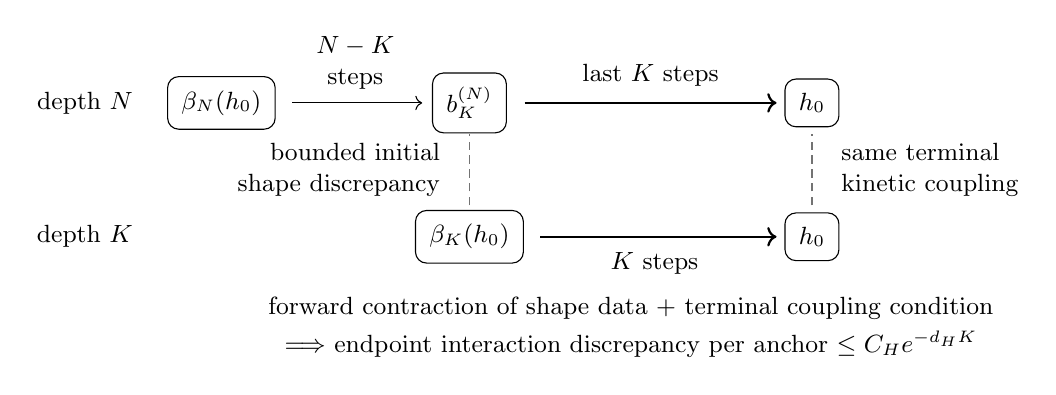
\begin{tikzpicture}[x=1cm,y=1cm,font=\small]
    \node[anchor=east] at (0,1.7) {depth $N$};
    \node[draw,rounded corners,inner sep=5pt] at (1.0,1.7)
      {$\beta_N(h_0)$};
    \draw[->] (1.9,1.7) -- (3.55,1.7);
    \node[above,align=center] at (2.7,1.75) {$N-K$\\steps};
    \node[draw,rounded corners,inner sep=5pt] at (4.15,1.7)
      {$b_K^{(N)}$};
    \draw[->,thick] (4.85,1.7) -- (8.05,1.7);
    \node[above] at (6.45,1.78) {last $K$ steps};
    \node[draw,rounded corners,inner sep=5pt] at (8.5,1.7) {$h_0$};

    \node[anchor=east] at (0,0) {depth $K$};
    \node[draw,rounded corners,inner sep=5pt] at (4.15,0)
      {$\beta_K(h_0)$};
    \draw[->,thick] (5.05,0) -- (8.05,0);
    \node[below] at (6.5,-0.08) {$K$ steps};
    \node[draw,rounded corners,inner sep=5pt] at (8.5,0) {$h_0$};

    \draw[densely dashed,black!55] (4.15,0.4) -- (4.15,1.3);
    \node[anchor=east,align=right] at (3.9,0.85)
      {bounded initial\\shape discrepancy};
    \draw[densely dashed,black!55] (8.5,0.4) -- (8.5,1.3);
    \node[anchor=west,align=left] at (8.75,0.85)
      {same terminal\\kinetic coupling};

    \node[align=center] at (6.2,-1.15)
      {forward contraction of shape data + terminal coupling condition\\[3pt]
       $\Longrightarrow$ endpoint interaction discrepancy per anchor $\le C_H e^{-d_H K}$};
  \end{tikzpicture}\par\medskip
  \caption{The comparison aligns the last $K$ blocking steps of two
  admitted trajectories with $N\ge K$. Here $b_K^{(N)}$ is the longer
  trajectory's coupling after its first $N-K$ steps. Their kinetic couplings agree
  at the terminal scale. Their complete endpoint laws need not agree:
  contraction bounds the discrepancy in their local interaction data,
  while bulk scalars are tracked separately. The bound is uniform in
  the number $N-K$ of earlier steps.}
  \label{fig:matched-trajectories}
\end{figure}

\FloatBarrier

\begin{theorem}[Matched endpoint densities]
\label{rg:matching}\label{thm:matched-endpoint}
Let $N\ge K\ge1$, and choose any two admitted nearest-neighbor
trajectories of these depths with the same terminal coupling
$h_0\in I_H$.  On every common admitted terminal period $m$,
write their exact endpoint densities as
\[
 \rho_r(V)=e^{v_rm^2}e^{X_r(V)}\Xi_r(V),\qquad r=N,K,
\]
using common compatible label lists.  The numbers $v_r$ are
independent of $m$.  There are constants $C_H,d_H>0$,
independent of $N,K,h_0,m$, such that
\begin{align}
 \|X_N-X_K\|_\infty
       &\le C_Hm^2e^{-d_HK},\nonumber\\
 \sup_x\sum_{\ell:x\in P_\ell}
      e^{As_\ell}\|k_{N,\ell}-k_{K,\ell}\|_\infty
       &\le C_He^{-d_HK}.
 \label{rg:terminal-difference}
\end{align}
All the endpoint class bounds hold uniformly.  In particular,
with $t=t_0$, the canonical part of $-X_r$ is bounded by
$C_Lm^2(Ht^4+t^2)$ and its error part by $m^2H^{-2.05}$.
Every covering support has a connected hull of at most
$R_Hs_\ell$ sites.  Changing a set $B$ of endpoint spins
changes $X_r$ by at most $D_H|B|$.  The constants $R_H,D_H$
can be chosen polynomial in $H$.
\end{theorem}
\begin{proof}
Compare the last $K$ layers, indexed by $j=K,\ldots,0$.
At their common upper layer both shape data are within the
fixed caps, so $u_K\le C$.  Their free histories differ;
the shallower one at layer $j$ is $K-j$, giving
$\epsilon_j\le L^{-(K-j)}$.  Their couplings agree at the
opposite end: $\lambda_0=0$.

Set $\eta=C_LH^{-b_*}$, enlarging its constant if necessary,
and $f_j=C_LH_j^CL^{-(K-j)}$.  The step inequalities imply
\[
 u_{j-1}\le q u_j+\eta|\lambda_j|+f_j,\qquad
 |\lambda_j|\le
 a|\lambda_{j-1}|+aC_Lu_j+af_j,\quad
 a=(1-\eta)^{-1}.
\]
Choose $\rho$ with $\max(q,L^{-1})<\rho<1$, and then
increase $H$ until $a\rho<1$.  Put
$w_j=\rho^{K-j}$,
$U=\max_{0\le j\le K}u_j/w_j$, and
$W=\max_{0\le j\le K}|\lambda_j|/w_j$.
For $F_K=C_{L,H}(1+K)^C$ we have $f_j\le F_Kw_j$.
Iterating the first inequality from $K$ and the second
from $0$ gives
\[
 U\le u_K+\frac{\eta W+F_K}{\rho-q},\qquad
 W\le\frac{a(C_LU+F_K)}{1-a\rho}.
\]
Choose $H$ so that the product of the two coefficients
linking $U$ and $W$ is less than $1/2$.
It follows that
\begin{equation}
 u_j+|\lambda_j|
       \le C_{L,H}(1+K)^C\rho^{K-j}.
 \label{rg:two-end-bound}
\end{equation}
This argument requires neither a bound on the ratio of
the two bare couplings nor uniqueness of either shot.

At $j=0$ the shape estimate and the free-history error
$O(L^{-K})$ give the covering estimate in
\eqref{rg:terminal-difference}.  They also bound the
regular negative-log difference per anchor, including
the difference of the clipped kinetic kernels; their
displayed couplings are equal.  Summing over $m^2$ anchors
gives the first estimate.  A fixed polynomial in $K$
is absorbed by decreasing the positive exponential rate.
Uniformity in $h_0$ follows from its compact admitted
interval and the same constants in the step estimates.

At each step only a bulk scalar was extracted.  The number
of sites at layer $j$ is $m^2L^{2j}$, so the sum of all
extracted scalars is exactly $v_rm^2$ with $v_r$ independent
of $m$.  All period discrepancies were kept in the winding
lists.

The remaining statements follow directly from the class
norms at $j=0$.  On a canonical graph,
$|y_o(x)|\le Ct$ times its path length; the exponential
coefficient norm sums the resulting fixed powers, giving
$C_L(Ht^4+t^2)$ per anchor.  The error bound is its cap.
The complete record gives a hull of $O(\mathfrak m_0^2s_\ell)$ sites.
For a local change of spins, sum only terms whose complete
support meets the changed set, charging each term to one
such site.  Conversion from anchored to support-hit sums
costs fixed position moments, and all test neighborhoods
have polynomial size in $H$.  The kinetic terms and their
mask tests obey the same bound by the free exponential
moments.  This gives $D_H$ polynomial in $H$.
\end{proof}

The endpoint densities in this theorem are strictly positive:
they are repeated integrals of the positive microscopic
density against the strictly positive kernel
\eqref{rg:observation}.  More quantitatively, changing $B$
endpoint spins changes the logarithm of the true endpoint
density by at most $C_LH|B|$.  For each fixed input the
last observation densities have this ratio bound, since
their coupling is in a fixed band of order $H$ and chord
lengths on $S^3$ are bounded.  Integrating their ratio
inequality against the positive preceding-layer measure
preserves it.  This positivity statement concerns the
complete density; the individual covering weights remain
allowed to have either sign.



\section{Relative comparison of the retained densities}
\label{cmp:section}

Closeness of the coefficients in an effective action does not by itself
compare the corresponding partition functions.  The difficulty here is
quite specific.  A retained density contains a signed covering sum, and
this sum can be small on configurations with many rough bonds.  Its
absolute difference is then an inadequate estimate for its relative
difference.

We prove the relative estimate by combining two facts.  Rough bonds are
rare under each of the two positive measures.  On the remaining
configurations, a local modification removes rough clusters at a
controlled cost.  An exact inclusion--exclusion identity then turns the
signed comparison into a convergent sum of trees.  Positivity will be
used for complete densities and complete covering sums, never for a
restricted signed sum.

\subsection{The finite-volume comparison problem}

Let
\[
 \Lambda_M=(\mathbb Z/M\mathbb Z)^2,\qquad v=|\Lambda_M|=M^2,
 \qquad q\in(S^3)^{\Lambda_M},
\]
where \(M\) is dyadic.  Write \(\dd q\) for product normalized Haar
measure, \(r_e=|q_x-q_y|\) for \(e=\langle xy\rangle\), and
\[
 D(q)=\{e:r_e>t_H\}.
\]
The large parameter \(H\) is the inverse coupling at the retained scale.
It is fixed throughout a comparison.  In the application,
\[
 t_H=H^{-1/2}p_H,\qquad p_H=(\log H)^{P_0},
\]
with the fixed exponent \(P_0\) chosen in the renormalization construction.

\begin{definition}[A mandatory covering sum]
\label{cmp:cover-definition}
A label \(\lambda\) consists of a finite site support \(P_\lambda\), a
load \(s_\lambda\ge1\), and a fixed nonempty inventory \(J_\lambda\) of
bonds whose endpoints belong to \(P_\lambda\).  Its weight
\(k_\lambda(q)\) is a bounded measurable function of \(q|_{P_\lambda}\);
every eligibility indicator is included in this function.  In
particular \(k_\lambda(q)=0\) unless \(J_\lambda\subset D(q)\).
The support contains every spin read by the function or by an
eligibility test, including a test asserting the absence of a flag.

A family is compatible when its supports are pairwise disjoint.  The
mandatory covering sum is
\begin{equation}
 \Xi(q)=
 \sum_{\substack{\Gamma\ {\rm compatible}\\
          \bigsqcup_{\lambda\in\Gamma}J_\lambda=D(q)}}
            \prod_{\lambda\in\Gamma}k_\lambda(q).
 \label{cmp:cover}
\end{equation}
The empty family has weight one.  Since inventories are nonempty,
\(\Xi(q)=1\) when \(D(q)=\varnothing\).
\end{definition}

The word mandatory refers to the equality of inventories in
\eqref{cmp:cover}.  In particular, \(\Xi\) is not the partition function
of an optional dilute gas.

Consider two pointwise positive densities
\begin{equation}
 \rho_i(q)=e^{X_i(q)}\Xi_i(q)>0,\qquad
 Z_i=\int\rho_i(q)\,\dd q,\qquad
 \dd\mu_i=Z_i^{-1}\rho_i\,\dd q,\quad i=1,2 .
 \label{cmp:densities}
\end{equation}
Use a common countable label set, putting unused weights equal to zero.
The functions in \eqref{cmp:densities} are the pointwise versions
provided by the exact blocking identity.

Here are the precise data needed for comparison.  A quantity described
as polynomial in \(H\) is bounded by \(CH^a\), with \(C,a\) fixed
independently of the period and the cutoff depths.

\begin{enumerate}
\item[\textup{(C1)}]
Each \(P_\lambda\) is contained in a connected lattice graph with at
most \(R_Hs_\lambda\) vertices, where \(R_H\) is polynomial in \(H\).
For a fixed \(A\ge16\),
\begin{align}
 \sup_x\sum_{\lambda:x\in P_\lambda}
          e^{As_\lambda}\|k_{i,\lambda}\|_\infty
       &\le w_H, \label{cmp:activity}\\
 \sup_x\sum_{\lambda:x\in P_\lambda}
          e^{As_\lambda}
          \|k_{2,\lambda}-k_{1,\lambda}\|_\infty
       &\le D_H\delta_K. \label{cmp:activity-difference}
\end{align}
Here \(w_H\) decreases faster than every inverse power of \(H\);
\(D_H<\infty\) is independent of the period and the cutoff depths.

\item[\textup{(C2)}]
If \(q,\widetilde q\) differ at \(n\) sites, then
\begin{align}
 |\log\rho_i(q)-\log\rho_i(\widetilde q)|
       &\le B_{\rho,H}n, \label{cmp:density-finite-energy}\\
 |X_i(q)-X_i(\widetilde q)|
       &\le B_{X,H}n, \label{cmp:exponent-finite-energy}
\end{align}
where \(B_{\rho,H},B_{X,H}\) are polynomial in \(H\).  Moreover
\begin{equation}
 \|X_2-X_1\|_\infty\le D_Hv\delta_K.
 \label{cmp:exponent-difference}
\end{equation}

\item[\textup{(C3)}]
For some \(c_*>0\) independent of \(H\),
\begin{equation}
 X_i(q)\le \epsilon_Hv-
                c_*H\sum_e\min(r_e^2,t_H^2),
 \qquad \epsilon_H=o(Ht_H^2).
 \label{cmp:stability}
\end{equation}
On the cap
\[
 {\cal C}_H=\{q:|q_x-\mathbf1|\le cH^{-1/2}
                         \text{ for every }x\},
\]
one has \(D(q)=\varnothing\) and
\begin{equation}
 X_i(q)\ge-\epsilon'_Hv,\qquad
 \epsilon'_H=o(Ht_H^2).
 \label{cmp:cap}
\end{equation}

\item[\textup{(C4)}]
Both positive measures are translation invariant and reflection
positive at the axis seams used to reflect lattice tiles.  The
reflection prescriptions are compatible with the tile events below.
Finally,
\[
 t_H\longrightarrow0,\qquad
 t_H^{-1}\le\operatorname{poly}(H),\qquad
 \frac{Ht_H^2}{(\log H)^2}\longrightarrow\infty .
 \label{cmp:thresholds}
\]
\end{enumerate}

All comparisons below are uniform over families satisfying these data.
The last subsection verifies the data for the retained densities of
Theorem~\ref{thm:rg-closure}.

\begin{theorem}[Relative comparison]
\label{thm:relative-comparison}
Suppose \textup{(C1)--(C4)} hold and
\(\delta_K\le C_H e^{-\gamma_H K}\), where \(\gamma_H>0\).
Fix \(0<\zeta_H<\gamma_H/2\).  For every sufficiently large fixed \(H\)
there are constants \(M_H,C_H,a_H>0\) such that, whenever \(M\ge M_H\),
there is a common measurable set \(G=G_{H,K,M}\) satisfying
\begin{align}
 \mu_i(G^c)&\le C_HM^2e^{-a_HK},\qquad i=1,2,
                    \label{cmp:bad-probability}\\
 \left|\frac{\Xi_2(q)}{\Xi_1(q)}-1\right|
   &\le \exp\!\left(C_HM^2\delta_K e^{\zeta_HK}\right)-1,
                       \qquad q\in G. \label{cmp:relative-cover}
\end{align}
The same estimate holds after interchanging \(1\) and \(2\).  Thus
\begin{equation}
 \left|\log\frac{\rho_2(q)}{\rho_1(q)}\right|
       \le C_HM^2\delta_K e^{\zeta_HK},\qquad q\in G.
 \label{cmp:relative-density}
\end{equation}
There are also \(c_H,d_H>0\) and \(K_H<\infty\) such that
\begin{equation}
 \left|\log\frac{Z_2}{Z_1}\right|\le C_He^{-d_HK}
 \quad\text{if}\quad
 K\ge K_H,\qquad M_H\le M,\qquad M^2\le e^{c_HK}.
 \label{cmp:partition-conclusion}
\end{equation}
\end{theorem}

\subsection{A joint rough-bond estimate under each positive law}

Choose a fixed constant \(C_1\), to be enlarged in the geometric
construction, and define the wider set of flagged bonds
\begin{equation}
 \widehat D(q)=\{e:r_e>t_H/C_1\}.
 \label{cmp:wider-flags}
\end{equation}
The distinction between \(D\) and \(\widehat D\) leaves room to modify a
configuration near its true rough bonds.

\begin{lemma}[Joint rarity]
\label{cmp:rarity}
For sufficiently large \(H\), there is
\(\sigma_H=cHt_H^2\), with \(c>0\) fixed after \(C_1\), such that
\begin{equation}
 \mu_i\{J\subset\widehat D\}\le e^{-\sigma_H|J|}
 \label{cmp:joint-rarity}
\end{equation}
for every set \(J\) of distinct bonds and \(i=1,2\).
\end{lemma}

\begin{proof}
Dropping the coverage and compatibility constraints only in an absolute
upper bound gives
\begin{equation}
 |\Xi_i(q)|
 \le\prod_\lambda(1+\|k_{i,\lambda}\|_\infty)
 \le\exp\!\left(\sum_\lambda\|k_{i,\lambda}\|_\infty\right)
 \le e^{vw_H}.
 \label{cmp:absolute-cover}
\end{equation}
All these sums converge by \eqref{cmp:activity}.  On \({\cal C}_H\) the
covering sum is exactly one.  A cap of radius \(cH^{-1/2}\) on \(S^3\)
has Haar measure at least \(c'H^{-3/2}\).  Consequently
\begin{equation}
 Z_i\ge
       \exp[-v(\epsilon'_H+C+\tfrac32\log H)].
 \label{cmp:denominator-cap}
\end{equation}

Place one specified flagged-bond event inside a \(2\)-by-\(2\) tile,
and reflect it into every tile.  The fully disseminated event requires
at least \(cv\) distinct flagged bonds.  On this event,
\(\sum_e\min(r_e^2,t_H^2)\ge c'vt_H^2\).  Equations
\eqref{cmp:stability}, \eqref{cmp:absolute-cover}, and
\eqref{cmp:denominator-cap} therefore imply
\begin{equation}
 \mu_i(\text{fully disseminated event})
 \le
 \exp\{-v[c''Ht_H^2-\epsilon_H-\epsilon'_H-w_H-C\log H]\}
 \le e^{-c'''vHt_H^2}.
 \label{cmp:disseminated}
\end{equation}

This is the classical chessboard estimate
\cite[Theorems 4.1--4.3]{FILS78}. To display the reflection hypotheses
used here, we include the following form of
successive Cauchy--Schwarz.  If \(f_z\) are nonnegative tile tests and
\(\theta_z f_z\) denotes their reflected placement in tile \(z\), then
\[
 \mu_i\!\left(\prod_z\theta_zf_z\right)
 \le
 \prod_z
 \mu_i\!\left(\prod_y\theta_y f_z\right)^{1/N_{\rm tile}}.
\]
At one seam, reflection positivity applies Cauchy--Schwarz to the two
half-torus functions.  It replaces them by their two reflected
duplicates and gives exponent \(1/2\) to each.  Repeat in each direction,
bisecting the dyadic array of tiles.  After all bisections a chosen tile
test has been reflected into every tile and has exponent
\(1/N_{\rm tile}\), which is the displayed inequality.

Partition \(J\) into finitely many orientation, parity, and tile-origin
classes.  One class contains at least a fixed fraction of its bonds,
with at most one specified test per tile.  Use the displayed inequality
with this test on those tiles and \(1\) elsewhere.  Applying
\eqref{cmp:disseminated} proves \eqref{cmp:joint-rarity}, after reducing
the constant in \(\sigma_H\).  This proof is performed separately for
each \(\mu_i\); it does not compare their normalizing constants.
\end{proof}

\subsection{Removing a rough cluster}

We first record the target-space fact used in the modification.

\begin{lemma}[Quantitative filling on \(S^3\)]
\label{cmp:filling}
An \(L_0\)-Lipschitz map from the boundary of the unit square to \(S^3\)
has an extension to the square with Lipschitz constant at most
\(C(1+L_0)^{3/2}\).  The extension can be chosen measurably as a function
of the boundary map.
\end{lemma}

\begin{proof}
Parameterize the boundary by a circle using a fixed bi-Lipschitz map
and write its image as \(g(\theta)\).  Its antipodal curve can be
covered by \(C(1+L_0/\eta)\) balls of radius \(2\eta\).  The total Haar
volume of these balls is at most
\(C(\eta^3+L_0\eta^2)\).  With
\(\eta=c(1+L_0)^{-1/2}\), this is smaller than the volume of \(S^3\).
Choose \(p\in S^3\) at distance at least \(c\eta\) from the antipodal
curve.  Then
\[
 F(r,\theta)=
 \frac{(1-r)p+rg(\theta)}{|(1-r)p+rg(\theta)|},
 \qquad 0\le r\le1,
\]
is well defined.  Indeed its denominator is bounded below by
\(c\eta\).  The radial derivative is \(O(\eta^{-1})\), and its angular
derivative is \(O(rL_0\eta^{-1})\).  In disk coordinates these imply the
claimed bound.  A fixed bi-Lipschitz map between disk and square changes
only the constant.

To make the choice measurable, fix a sufficiently fine finite net of
possible \(p\)'s and take the first one separated from the antipodal
curve by the smaller prescribed distance.  The volume argument with
slightly larger avoidance balls guarantees such a net point.
\end{proof}

\begin{lemma}[Disjoint editable regions]
\label{cmp:editing}
For fixed sufficiently large constants \(C_2,C_1\), in that order,
and \(M\ge M_H\), each configuration has a finite family of disjoint
editable site sets \(E_C\), with nonempty fixed inventories
\(D_C\subset D(q)\), such that
\[
 D(q)=\bigsqcup_C D_C.
\]
If \(n_C\) is the number of original flagged bonds assigned to this
region, then \(n_C\ge1\), the assigned flagged sets are disjoint, and
\begin{equation}
 |E_C|\le R_{E,H}n_C,\qquad
 E_C\text{ has a connected hull of at most }R_{E,H}n_C\text{ sites},
 \qquad R_{E,H}\le Ct_H^{-2}.
 \label{cmp:edit-size}
\end{equation}
One can replace the spins in any selected \(E_C\), leaving all other
spins and the region's outer boundary unchanged, so that every true
rough bond of \(D_C\) disappears and no true rough bond is created.
All choices can be made measurably.
\end{lemma}

\begin{proof}
Partition each coordinate circle into integer intervals of lengths
between \(\ell=\lceil C_2/t_H\rceil\) and \(2\ell\).  This is possible
once \(M\) exceeds a fixed multiple of \(\ell\).  Use the resulting
rectangular mesh.  Mark every box meeting a bond of \(\widehat D\).
Take the union of their closed two-box neighborhoods, and form
components by joining boxes that meet even at a vertex.  Distinct
components are disjoint closed mesh regions.  Keep just the components
containing a bond of \(D\).

Let \(E_C\) be the lattice sites in one retained region, and let \(n_C\)
count all originally flagged bonds whose marked boxes generate that
region.  A flagged bond marks only a bounded number of boxes, and each
marked box adds only a bounded number of boxes to its neighborhood.
Hence the number of boxes is at most \(Cn_C\), proving
\eqref{cmp:edit-size}.  The regions have a connected lattice hull with
the same bound.  Every flagged bond is separated from the boundary of
its component by a mesh collar.  Thus boundary bonds are unflagged.

Retain the original spins on all boundary vertices and edges of the
region.  Interpolate each such edge by short geodesic arcs between
successive lattice spins.  Its speed in physical lattice coordinates
is at most \(Ct_H/C_1\).  At every other mesh vertex choose the fixed
spin \(\mathbf1\).  On the other mesh sides join the chosen endpoint
spins by a fixed measurably selected shortest arc.  Use exactly the same
arc for the two cells sharing a side.

After rescaling a cell to the unit square, its boundary map has
Lipschitz constant at most \(C(1+C_2/C_1)\).  Apply
Lemma~\ref{cmp:filling} in every cell.  Choose \(C_2\) larger than the
resulting fixed filling constant for \(C_2/C_1\le1\), and then choose
\(C_1\) large enough.  The Lipschitz constant in lattice units is less
than \(t_H\).  Sampling the fillings at lattice sites therefore gives
new bond lengths below \(t_H\).

The fillings agree on shared sides.  Boundary spins were preserved,
so no bond crossing out of a region becomes rough.  The construction
also treats regions with holes.  If a region wraps around the torus,
the same shared-side rule is used periodically; if it fills the torus,
one may simply replace all its spins by \(\mathbf1\).
\end{proof}

Fix the regions and the modified values using the original
configuration, once and for all.  Write \({\cal I}\) for the retained
regions and \(q(I)\), \(I\subset{\cal I}\), for the configuration in
which precisely the regions outside \(I\) have been modified.  Then
\begin{equation}
 D(q(I))=\bigsqcup_{C\in I}D_C.
 \label{cmp:inventory-after-edit}
\end{equation}
The modification need not remove the wider flags at threshold
\(t_H/C_1\).  We never recluster a modified configuration; its geometry,
its \(n_C\)'s, and its inventories are those fixed from the original one.

Put \(\Xi_i(I)=\Xi_i(q(I))\).  Since \(\rho_i>0\), these are complete
positive sums.  Equations \eqref{cmp:density-finite-energy} and
\eqref{cmp:exponent-finite-energy} give the crucial denominator estimate:
\begin{equation}
 0<\frac{\Xi_i(I\setminus B)}{\Xi_i(I)}
 \le
 \exp\!\left(C_{3,H}\sum_{C\in B}n_C\right),
 \qquad
 C_{3,H}=(B_{\rho,H}+B_{X,H})R_{E,H}.
 \label{cmp:complete-ratio}
\end{equation}
Indeed \(\log\Xi_i=\log\rho_i-X_i\), and at most
\(R_{E,H}\sum_{C\in B}n_C\) sites have changed.

\subsection{Exact identities for the signed covering sums}

At a fixed active set \(I\), take a full original covering family and
join two of its labels whenever their supports meet the same active
region \(E_C\), \(C\in I\).  Call a connected group a macrolabel \(U\),
and give it support
\begin{equation}
 S_U=\bigcup_{\lambda\in U}P_\lambda
       \ \cup\
       \bigcup_{\substack{C\in I:\\
                    E_C\cap P_\lambda\ne\varnothing
                    \text{ for some }\lambda\in U}}E_C.
 \label{cmp:macro-support}
\end{equation}
Its weight is
\[
 w_i(U;q(I))=\prod_{\lambda\in U}k_{i,\lambda}(q(I)).
 \label{cmp:macro-weight}
\]
Every active region it meets is covered in full by this macrolabel:
all labels supplying its inventory meet that region and so belong to
the same group.  Different macrolabels have disjoint enlarged supports.
Conversely, compatible macrolabels covering all active inventories
recover exactly the original full covering families.

For a site set \(S\) disjoint from the active editable regions, let
\(\Xi_i(I;S)\) be the full-inventory sum restricted to macrolabels whose
supports avoid \(S\).  This restricted sum may have either sign.  If
\({\cal A}\) is a compatible selected macrolabel family, denote its
combined support by \(S_{\cal A}\), and the active regions it covers by
\(B_{\cal A}\).

\begin{lemma}[Removal and inclusion--exclusion]
\label{cmp:removal-identities}
The background left after selecting \({\cal A}\) has total weight
\begin{equation}
 \Xi_i(I\setminus B_{\cal A};S_{\cal A}).
 \label{cmp:background-identity}
\end{equation}
Consequently
\begin{align}
 \Xi_i(I;S)
 &=
 \sum_{\substack{{\cal A}\ {\rm compatible}\\
                   S_U\cap S\ne\varnothing\ \forall U\in{\cal A}}}
 (-1)^{|{\cal A}|}
 \left[\prod_{U\in{\cal A}}w_i(U;q(I))\right]
 \Xi_i(I\setminus B_{\cal A};S_{\cal A}),                 \label{cmp:IE}\\
 \Xi_2(I)-\Xi_1(I)
 &=
 \sum_{\substack{{\cal A}\ {\rm compatible}\\{\cal A}\ne\varnothing}}
 \left[\prod_{U\in{\cal A}}
       \bigl(w_2(U;q(I))-w_1(U;q(I))\bigr)\right]
 \Xi_1(I\setminus B_{\cal A};S_{\cal A}).                 \label{cmp:difference-identity}
\end{align}
The empty term in \eqref{cmp:IE} is \(\Xi_i(I)\).
\end{lemma}

\begin{proof}
The configurations \(q(I)\) and \(q(I\setminus B_{\cal A})\) differ
only inside \(S_{\cal A}\).  Every remaining weight and every
eligibility indicator reads a support avoiding this set, so its value
is unchanged.  A remaining active region is disjoint from
\(S_{\cal A}\), by the definition of \(B_{\cal A}\).  Removing the
selected regions therefore does not change the grouping of background
labels: background supports avoided these regions already.  Its
inventory requirement loses exactly the inventories in
\(B_{\cal A}\).  This proves the weight-preserving bijection
\eqref{cmp:background-identity}.

In every full covering family, expand the indicator that all its
macrolabels avoid \(S\) as
\[
 \prod_U\bigl(1-\mathbf1_{\{S_U\cap S\ne\varnothing\}}\bigr).
\]
After selecting the factors carrying the minus sign, apply
\eqref{cmp:background-identity}; this gives \eqref{cmp:IE}.  For
\eqref{cmp:difference-identity}, expand each product using
\(w_2=w_1+(w_2-w_1)\) and subtract the all-\(w_1\) term.

One may first perform these algebraic manipulations with finite label
lists.  A full family has at most \(|D(q(I))|\) original labels, and
\eqref{cmp:absolute-cover} provides absolute convergence of all the
unnormalized sums.  The identities therefore pass to the countable
lists.  Division by complete sums is performed only after this limit;
no positivity of a truncated or restricted sum is required.
\end{proof}

Introduce the nonnegative envelopes
\[
 p_\lambda=\|k_{1,\lambda}\|_\infty+
                         \|k_{2,\lambda}\|_\infty,\qquad
 d_\lambda=\|k_{2,\lambda}-k_{1,\lambda}\|_\infty
\]
and the restricted ratio
\[
 R_i(I,S)=\frac{|\Xi_i(I;S)|}{\Xi_i(I)}.
\]
Equations \eqref{cmp:complete-ratio} and \eqref{cmp:IE} give
\begin{equation}
 R_i(I,S)\le1+
 \sum_{\substack{{\cal A}\ne\varnothing,\ {\rm compatible}\\
                         S_U\cap S\ne\varnothing\ \forall U\in{\cal A}}}
 \left[\prod_{\lambda\in\bigcup{\cal A}}p_\lambda\right]
 e^{C_{3,H}\sum_{C\in B_{\cal A}}n_C}
 R_i(I\setminus B_{\cal A},S_{\cal A}).
 \label{cmp:ratio-recursion}
\end{equation}
A telescoping of each finite product also gives
\begin{equation}
 |w_2(U)-w_1(U)|
 \le\sum_{\lambda\in U}d_\lambda
                   \prod_{\substack{\kappa\in U\\\kappa\ne\lambda}}
                          p_\kappa .
 \label{cmp:marked-macro}
\end{equation}
Thus \eqref{cmp:difference-identity} starts the same recursion with a
nonempty first generation and one marked, differenced original label
in each of its macrolabels.  Every generation consumes at least one
active region.  The recursion is consequently finite.

\subsection{The common exceptional set}

Let \(C_{4,H}>0\) be a polynomial in \(H\), to be fixed in the next
subsection.  Define \(G\) by the following requirement.  Take any finite
collection of distinct original label nodes and distinct editable-region
nodes whose physical supports form a connected intersection graph.
Write
\[
 s=\sum_{\lambda}s_\lambda,\qquad n=\sum_C n_C.
\]
Whenever \(n>0\), require
\begin{equation}
 (C_{3,H}+C_{4,H})n\le \frac A4s+\zeta_HK.
 \label{cmp:good-set}
\end{equation}
This quantification uses the whole common label set, not just labels
eligible at the original configuration.  The recursion can evaluate a
label at a different \(q(I)\), and the same geometric inequality must
remain available there.  All these collections are countable, so \(G\)
is measurable.

\begin{lemma}[Probability of the exceptional set]
\label{cmp:exceptional}
For every polynomial choice of \(C_{4,H}\), sufficiently large \(H\)
admits an \(a_H>0\) such that
\begin{equation}
 \mu_i(G^c)\le2v e^{-a_HK},\qquad i=1,2 .
 \label{cmp:exceptional-bound}
\end{equation}
\end{lemma}

\begin{proof}
A violation of \eqref{cmp:good-set} implies
\[
 n>\frac{\zeta_HK}{C_{3,H}+C_{4,H}},\qquad
 s<\frac{4(C_{3,H}+C_{4,H})}{A}n.
\]
The connected hull bounds on labels and editable regions give a
connected graph containing these \(n\) distinct originally flagged
bonds, with at most \(B_Hn\) vertices and edges, for a polynomial
\(B_H\).  A traversal of this graph visits all the bonds with total
length at most \(CB_Hn\).

We count the ordered flagged bonds in such a traversal, rather than
every intervening lattice step.  There are at most \(2v\) choices for
the first bond.  At distance \(\ell\), there are at most
\(C(\ell+1)\) possible next bonds, including their orientations.
If \(Q\le CB_Hn\), the generating identity
\[
 \sum_{\ell\ge0}(\ell+1)z^\ell=(1-z)^{-2}
\]
therefore gives
\[
 \sum_{\ell_1+\cdots+\ell_n\le Q}
              \prod_{j=1}^n(\ell_j+1)
 =\binom{Q+2n}{2n}
 \le [C(1+B_H)^2]^n .
\]
This also bounds the number of ordered distinct-bond lists; allowing
repetitions in the count only increases it.  On a torus one may lift
the traversal before projecting its recorded bonds, which gives the
same upper bound.  Thus the number of possible flagged sets forced by
a violation is at most
\begin{equation}
 v[C(1+B_H)^2]^n .
 \label{cmp:flag-entropy}
\end{equation}
This estimate costs \(O(\log H)\) per flag, not \(O(B_H)\) per flag.

Set \(Q_H=C(1+B_H)^2e^{-\sigma_H}\).  Since \(B_H\) is polynomial and
\(\sigma_H=cHt_H^2\), assumption (C4) gives \(Q_H<1/2\) for large \(H\).
Lemma~\ref{cmp:rarity} and \eqref{cmp:flag-entropy} imply, under either law,
\[
 \mu_i(G^c)
 \le v\sum_{n>\zeta_HK/(C_{3,H}+C_{4,H})}Q_H^n
 \le2v e^{-a_HK},\qquad
 a_H=\frac{\zeta_H\log(1/Q_H)}{C_{3,H}+C_{4,H}}>0 .
\]
The possibly infinite number of labels adds no factor: every violating
collection already forces one of the flagged sets counted above.
\end{proof}

\subsection{A tree bound for the signed recursion}

We now prove the normalized estimate, including its combinatorial
multiplicity.

\begin{lemma}[Normalized covering comparison]
\label{cmp:forest}
For a sufficiently large polynomial \(C_{4,H}\) and sufficiently large
\(H\), the set \(G\) above satisfies
\begin{equation}
 \frac{|\Xi_2(q)-\Xi_1(q)|}{\Xi_1(q)}
 \le \exp(D_Hv\delta_K e^{\zeta_HK})-1 .
 \label{cmp:forest-conclusion}
\end{equation}
The same estimate holds with denominator \(\Xi_2(q)\).
\end{lemma}

\begin{proof}
Iterate \eqref{cmp:ratio-recursion} in
\eqref{cmp:difference-identity}, using \eqref{cmp:marked-macro}.  A term
is specified by successive nonempty compatible macrolabel families;
the recursion ends when the term \(1\) is chosen.  Every macrolabel
after the first generation meets the combined support of the preceding
generation.

Here is a faithful encoding of these terms by forests.  Inside each
macrolabel choose a spanning tree of its original label nodes and
editable-region nodes, using a fixed deterministic ordering to make the
choice.  For each later macrolabel choose, again deterministically, one
support intersection joining it to a macrolabel of the preceding
generation.  Color an edge according to whether it is internal to a
macrolabel or joins two generations.  Root each resulting tree at the
marked original label in its initial macrolabel.

No node is repeated.  An editable region is consumed the first time it
appears.  An original label has a fixed nonempty inventory; after it
appears, the regions containing that inventory have been removed, so
it cannot appear again in an eligible subsequent family.  Within one
generation supports are disjoint.

The encoding loses no multiplicity. Contract the internal edges to
recover each macrolabel, including its original labels and editable
regions. The depth of the resulting vertex in its rooted tree
recovers its generation; vertices at the same depth, across all trees,
recover the compatible family selected at that stage. The marked roots
recover the choices in the product telescoping. Finally, remove the
regions in all earlier generations to recover the active set \(I\) at
that stage and hence the configuration \(q(I)\) at which every weight
was evaluated. These data specify the original recursive term.
Thus two different terms cannot produce the same forest with its node
labels, marks and two edge colors. No ordering of siblings, or other
choice of a recursive history, remains to be counted.

Each tree is a connected collection of distinct nodes of the kind used
in \eqref{cmp:good-set}.  Its accumulated denominator factor is therefore
bounded by
\begin{equation}
 e^{C_{3,H}n}
 \le e^{\zeta_HK}
       \prod_{\lambda\ {\rm in\ the\ tree}}e^{As_\lambda/4}
       \prod_{C\ {\rm in\ the\ tree}}e^{-C_{4,H}n_C}.
 \label{cmp:tree-charge}
\end{equation}
The factor \(e^{\zeta_HK}\) occurs once per rooted tree.

To sum the remaining forests, give a gas node size \(s_\lambda\) and
an edit node size \(|E_C|\).  Their unmarked weights are
\[
 p_\lambda e^{As_\lambda/4},\qquad e^{-C_{4,H}n_C},
\]
respectively.  A marked gas root instead has weight
\(d_\lambda e^{As_\lambda/4}\).  Put \(R=\max(1,R_H)\) and choose
\begin{equation}
 C_{4,H}\ge2R_{E,H}+\log(16R)+1 .
 \label{cmp:C4}
\end{equation}
Since the editable sets are disjoint and \(n_C\ge1\),
\begin{equation}
 \sup_x\sum_{C:x\in E_C}
             e^{-C_{4,H}n_C}e^{2|E_C|}
       \le\frac1{16R}.
 \label{cmp:edit-hit}
\end{equation}
By \eqref{cmp:activity}, \(A/4+2\le A\), and the rapid decay of \(w_H\),
\begin{equation}
 \sup_x\sum_{\lambda:x\in P_\lambda}
           p_\lambda e^{As_\lambda/4}e^{2s_\lambda}
       \le2w_H\le\frac1{16R}.
 \label{cmp:gas-hit}
\end{equation}

A node of size \(a\) has support at most \(Ra\).  Summing a potential
child over one of its intersection sites and over the two edge colors,
equations \eqref{cmp:edit-hit}--\eqref{cmp:gas-hit} bound the child sum,
even with an exponential allowance for its descendants, by \(a/4\).
More explicitly, induction on maximum tree depth bounds the sum of
descendants below a root of size \(a\) by \(e^a\).  For the induction
step, each child of size \(b\) contributes at most its weight times
\(e^b\).  The sum over unordered distinct children is at most the
exponential of their one-child sum: sum ordered \(r\)-tuples with
factor \(1/r!\) and then drop distinctness.  The result is at most
\(e^{a/4}\le e^a\).  Positivity of these majorants permits the limit in
the maximum depth.

The marked-root sum is bounded by
\begin{equation}
 \sum_\lambda d_\lambda e^{As_\lambda/4}e^{s_\lambda}
       \le D_Hv\delta_K.
 \label{cmp:root-hit}
\end{equation}
Here summing the per-site bound can only overcount labels.  Actual
forest components have distinct marked roots.  Drop all disjointness
conditions between their descendant trees and sum unordered root sets.
Equations \eqref{cmp:tree-charge} and \eqref{cmp:root-hit} give
\[
 \sum_{\text{nonempty forests}}\text{majorant}
 \le \sum_{r\ge1}
       \frac{(D_Hv\delta_K e^{\zeta_HK})^r}{r!},
\]
which is \eqref{cmp:forest-conclusion}.

Every denominator used above was a complete positive \(\Xi_i(I)\);
every restricted signed sum entered only through its absolute value.
The argument is symmetric in \(1,2\), proving the last assertion.
\end{proof}

\subsection{From relative densities to partition functions}

\begin{lemma}[Normalization on a common set]
\label{cmp:normalization}
Let \(f_1,f_2>0\) be integrable, with \(0<Z_i=\int f_i\,\dd\nu<\infty\)
and \(\pi_i=f_i\nu/Z_i\).  If
\[
 \pi_i(G^c)\le\varepsilon_i<1,\qquad
 \left|\log\frac{f_2}{f_1}\right|\le\eta\quad\hbox{on }G,
\]
then
\begin{equation}
 e^{-\eta}(1-\varepsilon_1)
       \le\frac{Z_2}{Z_1}
       \le\frac{e^\eta}{1-\varepsilon_2}.
 \label{cmp:normalization-bound}
\end{equation}
If \(\varepsilon_i\le\varepsilon\le1/2\), then
\(\left|\log(Z_2/Z_1)\right|\le\eta+2\varepsilon\).
\end{lemma}

\begin{proof}
The relative density bound compares the two integrals over \(G\)
by factors \(e^{\pm\eta}\).  Use the exact identity
\[
 \frac{Z_2}{Z_1}
   =\frac{\int_G f_2\,\dd\nu}{\int_G f_1\,\dd\nu}
                       \frac{\pi_1(G)}{\pi_2(G)}.
\]
The last assertion follows from
\(-\log(1-\varepsilon)\le2\varepsilon\).
\end{proof}

\begin{proof}[Proof of Theorem~\ref{thm:relative-comparison}]
Choose \(C_{4,H}\) as in \eqref{cmp:C4}.  Lemma~\ref{cmp:exceptional}
gives the common exceptional-set estimate, and
Lemma~\ref{cmp:forest} gives \eqref{cmp:relative-cover}.

Applying the latter estimate in both directions yields
\[
 e^{-u}\le\frac{\Xi_2(q)}{\Xi_1(q)}\le e^u,\qquad
 u=D_Hv\delta_K e^{\zeta_HK}.
\]
This step does not require \(u\) to be small.
Adding \eqref{cmp:exponent-difference} proves
\eqref{cmp:relative-density}.

Let
\[
 b_H=\min(a_H,\gamma_H-\zeta_H)>0
\]
and choose \(0<c_H<b_H/2\).  If \(v\le e^{c_HK}\), both the exceptional
probability and the relative density error are at most
\(C_He^{-(b_H-c_H)K}\).  For \(K\) sufficiently large the former is
at most \(1/2\), so Lemma~\ref{cmp:normalization} proves
\eqref{cmp:partition-conclusion}, with any fixed
\(0<d_H\le b_H-c_H\) after adjusting \(C_H\).
\end{proof}

\subsection{Verification for the renormalized \(O(4)\) densities}

We now check the assumptions used in the theorem, including those that
come from positivity of the original model rather than from bounds on
its signed expansion.

At the retained scale, Theorem~\ref{thm:rg-closure} gives
\begin{equation}
 \rho_i=e^{X_i}\Xi_i,\qquad
 X_i=-h{\cal E}_i-{\cal P}_i-{\cal L}_i,\qquad
 H/2\le h\le2H.
 \label{cmp:RG-density}
\end{equation}
The two densities are written using the prescribed bulk scalar
normalization.  The kinetic form is
\begin{equation}
 {\cal E}_i(q)=\sum_e S_t(r_e)
           +\frac12\sum_e m_e(q)|(\ell_i\nabla q)_e|^2,
 \qquad
 S_t(r)=
 \begin{cases}
       c_0r^2/2,&r\le t,\\
       d_0tr,&r>t,
 \end{cases}
 \label{cmp:kinetic-form}
\end{equation}
where \(0<d_0<c_0/16\).  In this formula \(\nabla q\) denotes the field of
nearest-neighbor spin differences.  The free kernels \(\ell_i\) have
the stated uniform exponentially weighted row and column bounds.
Every mask and every other condition used by a term is part of its
complete support.

\paragraph{Support and difference norms.}
The complete-cover convention gives a connected hull with at most
\(C_L{\cal M}_H^2s_\lambda\) sites, where
\({\cal M}_H=\lceil(\log H)^2\rceil\).  Thus \(R_H\) is polynomial.
The covering bound is
\[
 w_H=\exp[-p_H^{1/4}],
\]
which decreases faster than every inverse power because \(P_0>4\).
The compatible lists and the equal-endpoint estimate of
Theorem~\ref{rg:matching} give
\eqref{cmp:activity-difference} and \eqref{cmp:exponent-difference}
with \(\delta_K\le C_He^{-\gamma_HK}\).  Any fixed polynomial in \(K\)
in that estimate is absorbed by decreasing \(\gamma_H\).
The constants are uniform in the longer cutoff depth and in the
admitted terminal coupling.

\paragraph{Strict positivity and finite energy of the full density.}
The last block observation has conditional density
\[
 Q_b(V\mid u)=z_{ab}^{-1}e^{abV\cdot u},\qquad |u|=1.
\]
In the small-mean branch it is a positive mixture of these densities
over constituent-spin directions.  In either case,
\begin{equation}
 e^{-2ab}\le\frac{Q_b(V\mid\cdot)}{Q_b(\widetilde V\mid\cdot)}
                     \le e^{2ab}.
 \label{cmp:kernel-ratio}
\end{equation}
For a mixture the bound follows term by term before summation.
The observation variables in different cells are conditionally
independent.  Changing \(n\) output spins therefore changes the product
kernel by a factor between \(e^{-2abn}\) and \(e^{2abn}\); integration
against any positive input density preserves this bound.

The incoming coupling in the last step is at most
\(2(H+\gamma_0)\), where \(\gamma_0=(\log L)/\pi\).  Hence
\[
 B_{\rho,H}=4a(H+\gamma_0)
\]
works in \eqref{cmp:density-finite-energy}, uniformly in all preceding
steps.  It also follows directly that the output density is strictly
positive.  Scalar extraction does not affect the ratio bound.

\paragraph{Reflection positivity.}
At a retained seam, the fine reflection exchanges the two disjoint
halves of the block partition.  The symmetric block weights, the
normalized-mean rule, and the constituent-spin fallback commute with
that reflection.  For a function \(F\) of output spins on one side,
let \({\cal Q}F\) be its conditional expectation given the input spins
on that side.  Conditional independence and reflection covariance give
\[
 \mu_{\rm out}((\theta\overline F)F)
   =\mu_{\rm in}
       ((\theta\overline{{\cal Q}F})\,{\cal Q}F)\ge0.
\]
Thus reflection positivity passes through each blocking step.
Translation and reflection compatibility on the retained lattice pass
through the same kernels.  Notice that conditional independence is
used together with reflection covariance.

\paragraph{Stability.}
The second term of \eqref{cmp:kinetic-form} is nonnegative and
\[
 h{\cal E}_i(q)\ge
           \frac{d_0H}{2}\sum_e\min(r_e^2,t_H^2).
\]
The seven canonical slots have degrees \(4,2,5,3,6,4,2\) and prefactors
\(h,1,h,1,h,1,h^{-1}\).  On a slot's regular mask, a displacement
along a recorded path of length \(u\) is at most \(ut_H\).
The exponential path norm absorbs every fixed power of \(u\), so
\begin{align*}
 \|{\cal P}_i\|_\infty
 &\le C_Lv\bigl(Ht_H^4+t_H^2+Ht_H^5+t_H^3
                         +Ht_H^6+t_H^4+H^{-1}t_H^2\bigr)\\
 &\le C_Lv(Ht_H^4+t_H^2).
\end{align*}
The regular-error norm gives
\(\|{\cal L}_i\|_\infty\le vH^{-2.05}\).  Thus
\eqref{cmp:stability} holds with
\[
 c_*=\frac{d_0}{2},\qquad
 \epsilon_H=C_L(Ht_H^4+t_H^2+H^{-2.05})=o(Ht_H^2).
\]
On the cap \({\cal C}_H\), all bonds are \(O(H^{-1/2})\), all masks
are on, and the row bound for \(\ell_i\) gives
\(h{\cal E}_i\le C_Lv\).  The same canonical and error estimates yield
\(X_i\ge-C_Lv\) there.  Since \(Ht_H^2\to\infty\), this is
\eqref{cmp:cap}.

\paragraph{Finite energy of the regular exponent.}
Changing \(n\) spins changes only \(O(n)\) direct bonds.  The row and
column bounds for \(\ell_i\) imply
\[
 \sum_e|(\ell_i\nabla(q-\widetilde q))_e|\le C_L n.
\]
A kinetic mask can change only if its read neighborhood meets a changed
bond.  Its radius is \(O(\log(2/t_H))\), so there are at most
\(C n\log^2(2/t_H)\) such masks.  Uniform boundedness of the row values
therefore bounds the kinetic variation by
\[
 C_LH[1+\log^2(2/t_H)]\,n.
\]
For the other terms, complete supports imply that a change is possible
only in terms whose supports hit a changed site.  Their exponential
path and cover norms bound this hit sum by a fixed polynomial in
\({\cal M}_H\) times their anchored norms: sum over possible anchors
in a connected hull, and absorb its fixed size powers with the spare
exponential weight.  It follows that
\[
 B_{X,H}\le C_LH[1+{\cal M}_H+\log(2/t_H)]^C,
\]
which proves \eqref{cmp:exponent-finite-energy}.

Finally \(t_H\to0\), \(t_H^{-1}\) is polynomially bounded, and
\(Ht_H^2=p_H^2\) dominates \((\log H)^2\).  This completes the
verification of (C1)--(C4).  Increasing the fixed minimum period to
accommodate the boxes in Lemma~\ref{cmp:editing} is harmless: it depends
only on \(H\), not on either cutoff depth.


\section{A fixed reference box and the lower mass bound}
\label{sec:assembly}

Fix $L$ and then $H$ large enough for all preceding estimates and
for $\varepsilon_H\le1/9$ in Lemma~\ref{lem:alignment}. This choice
precedes the selection of $K_0,M_0$ and is used for both mass bounds.
All estimates needed to compare different cutoffs have now been
established. We first make that comparison at the level of actual
partition functions, then choose the reference box only once.

Let $I_H$ be the terminal interval in Proposition~\ref{rg:admission}.
For an admitted $r$-step trajectory ending at $h\in I_H$, write its
initial coupling as $\beta_r(h)$. The exact integrations and the bulk
scalar convention give
\begin{equation}
\label{eq:blocked-partition}
 Z_{\beta_r(h)}(ML^r,ML^r)
   =e^{v_r(h)M^2}\mathcal Z_{r,h}(M),\qquad
 \mathcal Z_{r,h}(M)=\int f_{r,h,M}(V)\,\dd\nu_M(V).
\end{equation}
Here $\nu_M$ is product probability measure on the coarse $M\times M$
torus, $f_{r,h,M}$ is the complete positive density, and $v_r(h)$ is
independent of $M$. Only this last independence matters; the scalar
need not converge or be close for different depths.
The notation $\beta_r(h)$ does not assert uniqueness: every estimate
is uniform over all admitted trajectories with the specified endpoints.

\begin{proposition}[Comparison of cutoffs]
\label{prop:cutoff}
There are constants $C_H,c_H,d_H>0$ and a finite depth threshold such
that, for all admitted $N\ge K$, $h\in I_H$, and dyadic
$M\ge M_{\min}(L,H)$ with $(2M)^2\le e^{c_HK}$,
\begin{equation}
\label{eq:cutoff-comparison}
 |D_N(h;M)-D_K(h;M)|\le C_He^{-d_HK},\qquad
 D_r(h;M)=\Delta_{\beta_r(h)}(ML^r).
\end{equation}
The constants do not depend on the ratio of the two bare couplings or
on $N-K$.
\end{proposition}

\begin{proof}
Theorem~\ref{rg:matching} gives a local discrepancy
$\delta_K\le C_He^{-\gamma_HK}$ for the two terminal representations.
Apply Theorem~\ref{thm:relative-comparison} with their common terminal
coupling. There is one set $G$ such that, under each normalized law,
\[
 \mu_i(G^c)\le C_HM^2e^{-a_HK},
\]
and on $G$ the logarithms of the complete densities differ by at most
\[
 C_HM^2\delta_K e^{\zeta_HK},\qquad 0<\zeta_H<\gamma_H/2.
\]
This includes the regular exponent and the signed covering sum.
Choose $c_H<\min(a_H,\gamma_H-\zeta_H)$, and decrease it if any
admissible-volume restriction requires this. Both bounds then decrease
exponentially with $K$ whenever $M^2\le e^{c_HK}$.

Lemma~\ref{cmp:normalization}, which uses the exceptional probability
under both laws, consequently gives
\[
 |\log\mathcal Z_{N,h}(M)-\log\mathcal Z_{K,h}(M)|
                  \le C_He^{-d_HK}
\]
for some $d_H>0$ and all sufficiently large $K$.
The scalar in \eqref{eq:blocked-partition} cancels exactly:
\[
 D_r(h;M)=4\log\mathcal Z_{r,h}(M)-\log\mathcal Z_{r,h}(2M),
\]
because $4M^2-(2M)^2=0$. Apply the normalization bound at $M$ and $2M$;
the factor of five is absorbed in $C_H$.
\end{proof}

The size requirement is explicit in terms of the constants in the
construction. For a prescribed coarse box and error $\varepsilon$, it
suffices that
\begin{equation}
\label{eq:K-threshold}
 K\ge\max\left\{K_{\rm adm}(L,H),\frac{2\log(2M)}{c_H},
                        \frac{\log(C_H/\varepsilon)}{d_H}\right\},
 \qquad N\ge K.
\end{equation}
Here $K_{\rm adm}$ includes both trajectory admission and the lower
depth threshold in Proposition~\ref{prop:cutoff}.
Calibration gives
\begin{equation}
\label{eq:beta-depth}
 \beta_r(h)=\frac{\log L}{\pi}r+\frac1{2\pi}\log r+O_{L,H}(1).
\end{equation}
Thus the shorter depth controls the required largeness of both bare
inverse couplings. The proof gives finite thresholds through a specified
order of inequalities; it does not supply a useful numerical value for
them. The two trajectories must have the same terminal kinetic
coupling. Mere largeness of two arbitrarily chosen bare couplings is
not that matching condition.

\begin{theorem}[Lower bound]
\label{thm:lower}
There are fixed $K_0,M_0$, independent of the final depth, such that
\begin{equation}
\label{eq:lower-depth}
 \gap(\beta_N(h))\ge\frac{\log2}{M_0L^N},
 \qquad N\ge K_0,\quad h\in I_H.
\end{equation}
In particular $\gap(\beta)\ge c\sqrt\beta e^{-\pi\beta}$ for every
sufficiently large bare coupling, with $c>0$.
\end{theorem}

\begin{proof}
Temporarily let the reference depth $K$ grow. Choose a dyadic $M_K$ with
$\log M_K=K^{3/4}+O(1)$, and put $n_K=M_KL^K$.
Since $\log M_K=o(K)$, Proposition~\ref{prop:cutoff} admits $M_K$ and
$2M_K$ for all large $K$. By calibration and
Theorem~\ref{thm:preliminary}, uniformly for $h\in I_H$,
\[
 \log\frac{n_K}{\Xi(\beta_K(h))}
 =K^{3/4}-O_{L,H}(\sqrt{K\log K})\longrightarrow+\infty.
\]
The ratio grows faster than every polynomial in $K$, whereas the
logarithm of the polynomial prefactor in the preliminary estimate is
only $O_{L,H}(K)$. Hence
\[
 \sup_{h\in I_H}D_K(h;M_K)\longrightarrow0.
\]
Choose one finite $K_0$ for which all admissibility requirements hold
and
\[
 \sup_{h\in I_H}D_{K_0}(h;M_{K_0})+C_He^{-d_HK_0}\le2^{-10}.
\]
Fix $M_0=M_{K_0}$. The cutoff comparison now gives
$D_N(h;M_0)\le2^{-10}$ for every $N\ge K_0$.
Proposition~\ref{prop:criterion}, and uniqueness of the periodic limit
from Theorem~\ref{thm:preliminary}, prove \eqref{eq:lower-depth}.
Neither the reference depth nor the coarse box subsequently changes.

Finally, \eqref{eq:calibration} identifies $L^{-N}$ with
$\sqrt\beta e^{-\pi\beta}$ up to fixed positive factors.
Proposition~\ref{rg:admission} covers every sufficiently large bare
coupling, so this proves the last assertion.
\end{proof}

Figure~\ref{fig:fixed-reference-box} summarizes the order of choices.
\begin{figure}[tbp]
  \centering
  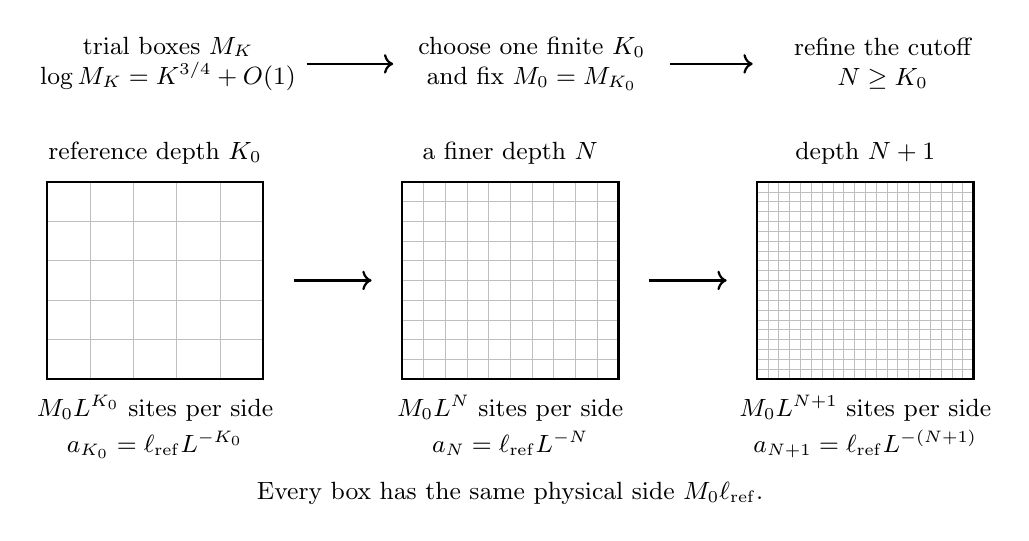
\begin{tikzpicture}[x=1.1cm,y=1cm,font=\small]
    \node[align=center] at (1.4,4.0)
      {trial boxes $M_K$\\$\log M_K=K^{3/4}+O(1)$};
    \draw[->,thick] (3.0,4.0) -- (4.0,4.0);
    \node[align=center] at (5.6,4.0)
      {choose one finite $K_0$\\and fix $M_0=M_{K_0}$};
    \draw[->,thick] (7.2,4.0) -- (8.15,4.0);
    \node[align=center] at (9.65,4.0)
      {refine the cutoff\\$N\ge K_0$};

    \begin{scope}[shift={(0,0)}]
      \draw[step=0.5,black!25,very thin] (0,0) grid (2.5,2.5);
      \draw[thick] (0,0) rectangle (2.5,2.5);
      \node[above] at (1.25,2.6) {reference depth $K_0$};
      \node[align=center,below] at (1.25,-0.08)
        {$M_0L^{K_0}$ sites per side\\[2pt]$a_{K_0}=\ell_{\mathrm{ref}}L^{-K_0}$};
    \end{scope}
    \draw[->,thick] (2.85,1.25) -- (3.75,1.25);
    \begin{scope}[shift={(4.1,0)}]
      \draw[step=0.25,black!25,very thin] (0,0) grid (2.5,2.5);
      \draw[thick] (0,0) rectangle (2.5,2.5);
      \node[above] at (1.25,2.6) {a finer depth $N$};
      \node[align=center,below] at (1.25,-0.08)
        {$M_0L^N$ sites per side\\[2pt]$a_N=\ell_{\mathrm{ref}}L^{-N}$};
    \end{scope}
    \draw[->,thick] (6.95,1.25) -- (7.85,1.25);
    \begin{scope}[shift={(8.2,0)}]
      \draw[step=0.125,black!25,very thin] (0,0) grid (2.5,2.5);
      \draw[thick] (0,0) rectangle (2.5,2.5);
      \node[above] at (1.25,2.6) {depth $N+1$};
      \node[align=center,below] at (1.25,-0.08)
        {$M_0L^{N+1}$ sites per side\\[2pt]$a_{N+1}=\ell_{\mathrm{ref}}L^{-(N+1)}$};
    \end{scope}
    \node at (5.35,-1.45)
      {Every box has the same physical side $M_0\ell_{\mathrm{ref}}$.};
  \end{tikzpicture}\par\medskip
  \caption{The order of choices in the lower-bound argument.
  The growing family of trial boxes is used only to select one
  reference depth and one coarse period. The comparison then transfers
  the small square-box test to all finer admitted cutoffs at the same
  terminal coupling. The grids are schematic; their counts are not
  the actual lattice periods. Refinement does not enlarge the physical
  reference box.}
  \label{fig:fixed-reference-box}
\end{figure}


The exponent $3/4$ is only a convenient choice between $1/2$ and $1$.
More generally an error $o(\beta)$ in the logarithm of the preliminary
length can be absorbed in a subexponentially growing reference box.
Calibration fixes the physical size of a coarse cell; comparison
transfers a small partition-function test to a fixed number of those
cells. Both facts are needed for the bound.


\FloatBarrier
\section{An upper bound from correlated block observables}
\label{sec:upper}

A lower bound for the full gap must exclude all low-energy sectors.
For an upper bound one nonvanishing correlation at a controlled
distance suffices. We obtain such a correlation from the terminal
spins, then pull it back through the observation kernels to two bounded
observables of the original spins. The only estimate from
Section~\ref{cmp:section} needed here is the one-law rarity bound of
Lemma~\ref{cmp:rarity}. Its proof uses (C1), (C3), and (C4), already
verified for each retained density; it uses neither relative comparison
of two densities nor matching of their terminal couplings.

\subsection{Alignment and the microscopic observables}

\begin{lemma}[Alignment of retained spins]
\label{lem:alignment}
For the actual retained densities of Theorem~\ref{thm:rg-closure},
uniformly in the cutoff depth and the admitted terminal coupling,
\begin{equation}
\label{cmp:alignment}
 \mathbb E|V_X-V_{X+e}|^2\le\varepsilon_H,\qquad
 \varepsilon_H=(t_H/C_1)^2+4e^{-\sigma_H}
                         \longrightarrow0\quad(H\to\infty).
\end{equation}
If $H$ is large enough that $\varepsilon_H\le1/9$, then
\begin{equation}
\label{cmp:block-correlation}
 \mathbb E[V_0^{(1)}V_{3e}^{(1)}]\ge\frac18.
\end{equation}
At depth $N$ this is the correlation of two centered original-spin
observables of norm at most one, supported in their respective
ancestral blocks of side $L^N$.
\end{lemma}

\begin{proof}
Apply Lemma~\ref{cmp:rarity} to a single bond. Outside its flagged
event the squared chord is at most $(t_H/C_1)^2$, and everywhere
it is at most $4$. This proves \eqref{cmp:alignment}.
Along three consecutive bonds, Cauchy--Schwarz gives
\[
 \mathbb E|V_0-V_{3e}|^2
 \le3\sum_{j=0}^2
       \mathbb E|V_{je}-V_{(j+1)e}|^2
 \le9\varepsilon_H.
\]
The spins are unit vectors, so
$\mathbb E[V_0\cdot V_{3e}]\ge1-9\varepsilon_H/2\ge1/2$.
The exact joint law is $O(4)$-invariant. Therefore every component
has mean zero and
$\mathbb E[V_0^{(1)}V_{3e}^{(1)}]
      =\frac14\mathbb E[V_0\cdot V_{3e}]$, proving
\eqref{cmp:block-correlation}.

Condition on the original spins $\sigma$, and define
\begin{equation}
\label{eq:block-observable}
 F_X(\sigma)=\mathbb E[V_X^{(1)}\mid\sigma],\qquad
 \|F_X\|_\infty\le1.
\end{equation}
Each observation kernel reads only the spins in its block. Iterating
this fact, all auxiliary observation variables and fallback tags that
produce $V_X$ lie in its ancestral block. Distinct ancestral blocks
use disjoint auxiliary variables, independent conditional on $\sigma$.
Integrating these block trees shows that $F_X$ depends only on the
original spins in its block and $\mathbb E F_X=0$. For disjoint blocks,
\[
 \mathbb E[F_XF_Y]=\mathbb E[V_X^{(1)}V_Y^{(1)}].
\]
In particular, choosing $e=e_1$ in the time direction gives
\begin{equation}
\label{eq:block-correlation}
 \mathbb E[F_0F_{3e_1}]\ge1/8.
\end{equation}
\end{proof}

The finite-torus conclusion passes to the periodic infinite-volume
state at each fixed depth $N$. To justify this even for a measurable
fallback rule, approximate the bounded local functions $F_X$ and
their products by continuous functions in product-Haar $L^1$.
The nearest-neighbor model has finite-support marginal densities
bounded uniformly in the surrounding torus, with a bound depending
only on that fixed support and its fixed bare coupling; this follows
by bounding the finitely many incident interaction terms in its
conditional density. The approximation is therefore uniform in the
torus size. Local convergence then proves the claim. This passage
uses no continuum construction.

\subsection{Transfer across the actual support gap}

The choice of $H$ at the start of Section~\ref{sec:assembly} already
ensures $\varepsilon_H\le1/9$. It remains to compare the correlation
\eqref{eq:block-correlation} with the distance between the two
microscopic supports.

We will use the following direct consequence of the full transfer gap.
If real centered bounded observables $F,G$ are supported in time slabs
$[-r,0]$ and $[d,d+s]$, respectively, then
\begin{equation}
\label{eq:actual-slab}
 |\Cov(F,G)|\le\norm F_\infty\norm G_\infty e^{-\gap d}.
\end{equation}
Indeed let $\theta$ reflect in the zero-time plane, and translate $G$
by $-d$. Their half-space vectors satisfy
$\Cov(F,G)=\langle[\theta F],T^d[\tau_{-d}G]\rangle$.
Each vector has norm at most its sup norm, by the reflected
expectation defining that norm. Both vectors are perpendicular to the
vacuum. Applying the definition of $\gap$ proves
\eqref{eq:actual-slab}. Bounded measurable observables follow by local
$L^2$ approximation and Cauchy--Schwarz. This argument uses the actual
infinite-volume Hilbert space and makes no claim that finite-cylinder
eigenvalues converge individually.

\begin{proposition}[Upper bound]
\label{prop:upper}
For all the admitted trajectories used above,
\begin{equation}
\label{eq:upper-depth}
 \gap(\beta_N(h))\le(\log8)L^{-N}.
\end{equation}
\end{proposition}

\begin{proof}
The observables in \eqref{eq:block-observable} are centered and bounded
by one. Their ancestral blocks, indexed by $0$ and $3e_1$, are
separated by at least $L^N$ time steps, as shown in
Figure~\ref{fig:block-supports}. Apply \eqref{eq:actual-slab} to
\eqref{eq:block-correlation} to get
$1/8\le e^{-\gap(\beta_N(h))L^N}$, which proves the result.
\end{proof}

\begin{figure}[tbp]
  \centering
  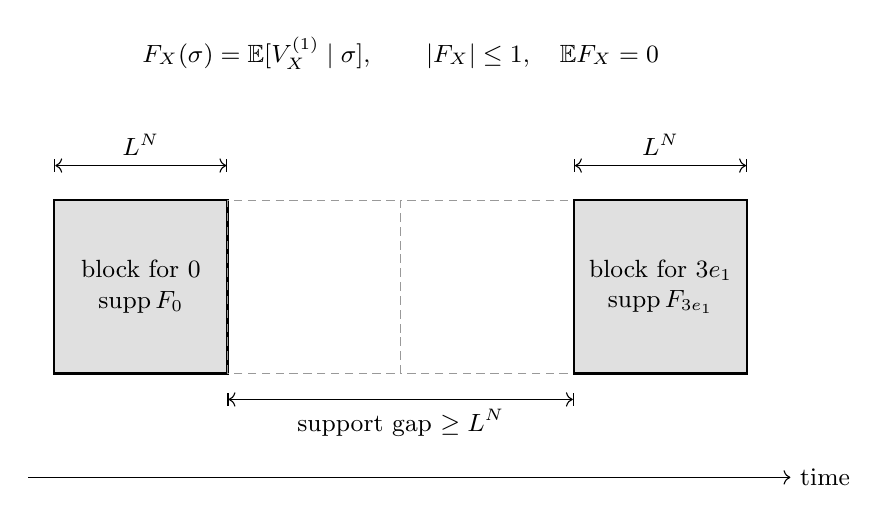
\begin{tikzpicture}[x=2.2cm,y=2.2cm,font=\small]
    \draw[fill=black!12,thick] (0,0) rectangle (1,1);
    \draw[densely dashed,black!40] (1,0) rectangle (2,1);
    \draw[densely dashed,black!40] (2,0) rectangle (3,1);
    \draw[fill=black!12,thick] (3,0) rectangle (4,1);
    \node[align=center] at (0.5,0.5) {block for $0$\\$\operatorname{supp} F_0$};
    \node[align=center] at (3.5,0.5)
      {block for $3e_1$\\$\operatorname{supp} F_{3e_1}$};

    \draw[|<->|] (0,1.2) -- (1,1.2);
    \node[above] at (0.5,1.2) {$L^N$};
    \draw[|<->|] (3,1.2) -- (4,1.2);
    \node[above] at (3.5,1.2) {$L^N$};
    \draw[|<->|] (1,-0.15) -- (3,-0.15);
    \node[below] at (2,-0.15) {support gap $\ge L^N$};
    \draw[->] (-0.15,-0.6) -- (4.25,-0.6);
    \node[anchor=west] at (4.25,-0.6) {time};

    \node at (2,1.85)
      {$\displaystyle F_X(\sigma)=\mathbb E[V_X^{(1)}\mid\sigma],
       \qquad |F_X|\le1,\quad \mathbb E F_X=0$};
  \end{tikzpicture}\par\medskip
  \caption{Pulling terminal observables back to the original lattice.
  Each displayed support lies within an ancestral block of side $L^N$.
  The auxiliary block variables are independent between disjoint
  ancestral blocks conditional on the original spins, so
  $\mathbb E[F_0F_{3e_1}]=\mathbb E[V_0^{(1)}V_{3e_1}^{(1)}]$.
  Alignment bounds this correlation below by $1/8$; the full transfer
  gap bounds it above by the exponential of minus the gap times $L^N$.
  No independence of the two pulled-back observables is asserted.}
  \label{fig:block-supports}
\end{figure}


\begin{proof}[Completion of Theorem~\ref{thm:main}]
Theorem~\ref{thm:preliminary} gives existence and uniqueness of the
periodic local limit. Proposition~\ref{rg:admission} supplies all
required trajectories and covers every sufficiently large bare
coupling. Theorem~\ref{thm:lower} and Proposition~\ref{prop:upper}
give the two bounds in depth units. Proposition~\ref{prop:calibration}
converts them to \eqref{eq:target}. Every choice of constants was made
before the final depth $N$.
\end{proof}

\FloatBarrier
\section{Physical units and the role of a continuum limit}
\label{sec:physical}

Choose a physical reference length $\ell_{\mathrm{ref}}>0$ and terminal
coupling $h=H$. A microscopic time separation of $n$ steps then equals
$a_Nn$, with $a_N=\ell_{\mathrm{ref}}L^{-N}$. Since
$e^{-\gap n}=e^{-(\gap/a_N)(a_Nn)}$, the mass in these units is
$m_{{\rm phys},N}=\gap(\beta_N(H))/a_N$. The proved bounds are
\begin{equation}
\label{eq:physical-bounds}
 \boxed{\displaystyle
  \frac{\log2}{M_0\ell_{\mathrm{ref}}}
  \le m_{{\rm phys},N}\le\frac{\log8}{\ell_{\mathrm{ref}}},
       \qquad N\ge K_0.}
\end{equation}
These are uniform bounds for cutoff theories. They require neither
convergence of their measures nor convergence of the numerical sequence
of masses. Equally, if one prescribes
$a(\beta)\Lambda=A\sqrt\beta e^{-\pi\beta}(1+o(1))$ with positive
fixed $A,\Lambda$, Theorem~\ref{thm:main} bounds the physical mass above
and below by positive multiples of $\Lambda$.

The half-logarithm in \eqref{eq:calibration} matters. Write
$\xi_{\rm lat}=\gap^{-1}$ for the inverse full gap. Knowing only
$\log\xi_{\rm lat}/\beta\to\pi$ would also allow
$\xi_{\rm lat}=\beta^{-1/2}e^{\pi\beta+\sqrt\beta}$, whose inverse
vanishes in these physical units. Our proof bounds the entire
multiplicative error.

\subsection{What would pass to an existing continuum theory}

We state separately the precise spectral implication if an appropriate
continuum limit is available. This is not used to prove
\eqref{eq:physical-bounds}.

\begin{proposition}
\label{prop:continuum}
Let $a_j\downarrow0$ and let $T_j$ be positive lattice transfer
contractions with normalized vacua $\Omega_j$ and full gaps $m_j$ satisfying
$\liminf_jm_j/a_j\ge m_*>0$. Suppose a limiting theory has Hilbert
space $\HH$, normalized vacuum $\Omega$, and a strongly continuous semigroup
$e^{-t\mathsf H}$ with $\mathsf H\ge0$ self-adjoint and
$\mathsf H\Omega=0$. Suppose a set of centered vectors $u$ dense in
$\Omega^\perp$ has
centered lattice approximants $u_j\perp\Omega_j$ and nonnegative
integers $n_j(t)$ such that
\[
 \norm{u_j}^2\to\norm u^2,\qquad
 \langle u_j,T_j^{n_j(t)}u_j\rangle
       \to\langle u,e^{-t\mathsf H}u\rangle,
 \qquad a_jn_j(t)\to t
\]
for every $t\ge0$. Then
\[
 \spec(\mathsf H)\subset\{0\}\cup[m_*,\infty),\qquad
 \ker\mathsf H=\C\Omega.
\]
\end{proposition}

\begin{proof}
For every $t>0$, the lattice gap gives
\[
 \langle u_j,T_j^{n_j(t)}u_j\rangle
 \le e^{-(m_j/a_j)a_jn_j(t)}\norm{u_j}^2.
\]
Pass to the limit and extend by density. For every $u\perp\Omega$,
$\langle u,e^{-t\mathsf H}u\rangle\le e^{-m_*t}\norm u^2$.
Positivity of its spectral measure excludes spectral weight below
$m_*$, including at zero, on that subspace.
\end{proof}

The norm convergence can instead be imposed after positive-time
regularization. More precisely, for each $u$ in a dense subset of
$\Omega^\perp$, suppose there are centered lattice vectors $v_j$ and
some $s>0$. Define their autocorrelations by
\[
 C_j(t)=\langle v_j,T_j^{\lfloor t/a_j\rfloor}v_j\rangle
 \qquad(t\ge0),
\]
and assume that
\[
 C_j(s+r)\longrightarrow\langle u,e^{-r\mathsf H}u\rangle
 \quad(r\ge0).
\]
The case $r=0$ gives $C_j(s)\to\|u\|^2$. For $t>s$, positivity of
the lattice spectral measure gives
$C_j(t)\le e^{-(m_j/a_j)(t-s+o(1))}C_j(s)$.
Apply this with $t=s+r$ and pass to the limit to obtain the same
quadratic-form bound as in the proposition. Thus no bound on
$\|v_j\|$, or on an unnormalized field renormalization constant,
is needed. Euclidean covariance is a separate condition if the energy
gap is to be interpreted as a relativistic mass gap.

An upper bound needs a surviving observable. Low-energy cutoff states
can disappear from a chosen limiting Hilbert space: the positive energy
measures $j^{-1}\delta_1+(1-j^{-1})\delta_R$, $R>1$, have spectral
bottom one but converge to $\delta_R$. A sufficient observable-survival condition is the following: in the
same limiting theory there are centered vectors $f,g$, with
$\|f\|,\|g\|\le1$, and a time separation $d\ge\ell_{\mathrm{ref}}$,
such that the separated cutoff block cross correlations converge to
$\langle f,e^{-d\mathsf H}g\rangle\ge1/8$. Then, writing
$m_{\mathrm{cont}}$ for the spectral bottom on $\Omega^\perp$,
\[
 1/8\le |\langle f,e^{-d\mathsf H}g\rangle|
 \le e^{-dm_{\mathrm{cont}}}
 \le e^{-\ell_{\mathrm{ref}}m_{\mathrm{cont}}},
\]
so $m_{\mathrm{cont}}\le(\log8)/\ell_{\mathrm{ref}}$.
The mixed-correlation convergence and norm bounds are additional
hypotheses; separate convergence of observables without these properties
would not suffice. These convergence requirements identify the
additional input for a statement about a continuum spectrum. The
finite and positive mass bounds in physical units have already been
proved without that input.

\appendix
\section{Uniform analytic estimates for the linear block map}
\label{app:analytic-block}

This section supplies the analytic estimates used in the linear block
transformation.  In particular, every strip width and every constant below
is chosen independently of the blocking depth and before the sufficiently
large integer $L$ is chosen.  There are only finitely many derivative and
decay orders in an application of these estimates.

\subsection{Domains, sampling, and the free precision}

We use integer site coordinates for Fourier transforms.  Changing to
block-centered coordinates conjugates the formulas by deterministic
translation phases; in coarse momentum these phases and their fixed
derivatives are uniformly bounded.  The integer-coordinate convention
makes the gluing of aliases explicit.  For $\delta>0$, put
\[
 \Omega_\delta=\{p\in\mathbb C^2:
       |\mathop{\rm Re}p_\mu|<\pi+\delta,\quad
       |\mathop{\rm Im}p_\mu|<\delta\}.
\]
An alias field is a family on these overlapping cubes, with the alias
index relabeled when $p$ crosses a face of the real momentum cube.
Equivalently it is a function of $k$ on the fine momentum torus, with
$p=Lk$ reduced modulo $2\pi$.  At a centered representative $l$ write
$\langle l\rangle=1+|l|_1$.  The weights of two representatives used
on an overlap are comparable by an absolute constant.  All estimates
on overlapping cubes therefore define estimates of the same field.
An analytic star means $f^*(z)=\overline{f(\bar z)}$ for real-kernel
matrix symbols, with transposition included for matrices; for the
scalar Fourier transform of real weights it is $b^*(z)=b(-z)$.

\begin{lemma}[Uniform shells and strips]\label{app:free-strip}
For the sampled smooth block weights in Section~\ref{free:section},
there are $\delta,c,C>0$ and $L_0$ with the following properties for
$L\ge L_0$ and $h\ge0$.  The precisions $K_h$ and an elliptic edge lift
$B_h$ are analytic on the complex $\delta$-neighborhood of the momentum
torus.  On the real torus,
\[
 cD\le K_h\le CD,\qquad cI\le B_h\le CI,
 \qquad K_h=d^*B_hd,\quad B_h(0)=I.
\]
Their fixed derivatives are bounded, $K_h-D$ has a zero of order four
at zero, and their history differences, including the inverse edge
lifts, are bounded by $CL^{-h}$ when compared with any depth
$\bar h\ge h$.  The same assertions hold on a common smaller strip.
\end{lemma}

\begin{proof}
Let $s_L=\sum_xb_x^2$.  Smoothness and normalization of the sampled
bump give $s_L\le A/L^2$ for a fixed $A$.  Discrete summation by parts
$N$ times, with no boundary terms because the bump is supported in the
block interior, gives
\begin{equation}
 |\partial_p^\alpha b((p+2\pi l)/L)|
       \le C_{N,\alpha}\langle l\rangle^{-N}
       \quad(p\in\Omega_{\delta_0}).                 \label{app:analytic-1}
\end{equation}
Here $\delta_0>0$ can initially be any sufficiently small fixed
constant.  Indeed the sum of absolute $N$th differences of the
normalized weights is $O(L^{-N})$, whereas on a nonzero alias at
least one difference multiplier has size $c\langle l\rangle/L$.
Complex tilting costs at most $\exp(C\delta_0)$, since the block has
diameter $O(L)$; derivatives in $p$ insert bounded rescaled coordinates.
The principal alias is bounded directly.  This also proves \eqref{app:analytic-1} in
the centered convention.

Set $m=L^h$, $W_h(\xi)=\prod_{j=1}^h b(\xi/L^j)$ and
$D_m(\xi)=m^2D(\xi/m)$.  For centered $l\ne0$ modulo $m$,
\begin{equation}
 |D_m(p+2\pi l)|\ge c\langle l\rangle^2
                    \quad(p\in\Omega_{\delta_0}),       \label{app:analytic-2}
\end{equation}
after reducing $\delta_0$.  To check the complex bound directly,
use $D_m(z)=4m^2\sum_\mu\sin^2(z_\mu/(2m))$.
Its real part is at least $c|\mathop{\rm Re}z|^2-C|\mathop{\rm Im}z|^2$
on this cube.  A nonzero alias has
$|\mathop{\rm Re}(p+2\pi l)|\ge c\langle l\rangle$.
This proves \eqref{app:analytic-2}, including aliases at the faces of the cube.

Here is a precise shell estimate, including its complex tilt.  The
$r$-fold block weights have squared sum $s_L^r$: the base-$L$
representation of each position in an $L^r$ block is unique.  Their
positions divided by $L^r$ remain in a fixed bounded square.  Finite
Fourier orthogonality, first at tilt $+\mathop{\rm Im}p$ and then at
tilt $-\mathop{\rm Im}p$, and Cauchy--Schwarz give
\begin{equation}
 \sum_{l\bmod L^r}
 |W_r(p+2\pi l)W_r(p+2\pi l)^*|\le C A^r.             \label{app:analytic-3}
\end{equation}
For a shell contained in $|l|_\infty\le L^r/2$, the factors with
$j>r$ have absolute product at most a fixed constant: their real
arguments cost at most one and their complex tilts cost
$\exp(C\delta_0\sum_{j>r}L^{1-j})$.  Thus \eqref{app:analytic-3} bounds the
corresponding shell of $W_h$ too.  Split the nonprincipal aliases
into the first shell $0<|l|_\infty\le L/2$ and the shells
$L^{r-1}/2<|l|_\infty\le L^r/2$, $2\le r\le h$.
Equations \eqref{app:analytic-2}--\eqref{app:analytic-3} imply
\begin{equation}
 \sum_{l\ne0}
 \left|\frac{W_h(p+2\pi l)W_h(p+2\pi l)^*}
 {D_m(p+2\pi l)}\right|
 \le C\sum_{r=1}^h\frac{A^r}{L^{2(r-1)}}\le C,        \label{app:analytic-4}
\end{equation}
uniformly once $L^2\ge2A$.  The noise sum
$a^{-1}\sum_{r<h}s_L^r$ is also bounded.  Consequently the function
$R_h$ in \eqref{free:explicit} is bounded on a fixed complex domain.
Cauchy's estimate on nested fixed domains bounds every required fixed
derivative; no real-momentum estimate is being used in place of a
complex estimate.

For real $p$ in the cube, the centered one-dimensional bump has phase
variation less than $\pi/2$ in its first principal factor.  The
product structure gives $|b(p/L)|\ge c$.
For $j\ge2$,
$1-b(p/L^j)b(p/L^j)^*=O(|p|^2L^{-2(j-1)})$.
It follows that $W_h(p)W_h(p)^*\ge c$ uniformly in $h$.
The denominator
\[
 F_h(p)=W_h(p)W_h(p)^*+D_m(p)R_h(p)
\]
is therefore at least $c$ on the real cube.  It and its first
derivatives have uniform bounds on the larger complex cube.  A
fixed reduction of the imaginary width gives $|F_h|\ge c/2$.
The formula $K_h=D_m/F_h$ now proves analyticity and boundedness.
The defining covariance sum proves that expressions from overlapping
alias cubes agree.  Real ellipticity follows from \eqref{app:analytic-4}, and the
expansions $F_h=1+O(|p|^2)$,
$D_m=|p|^2+O(|p|^4/m^2)$ give $K_h-D=O(|p|^4)$.

For completeness, history differences require no division by a bump
factor.  On common aliases $|l|_\infty\le L^h/2$ put
$\xi=p+2\pi l$.  Taylor's theorem for the extra product, with the
linear term canceled in each $bb^*$, gives
\[
 |W_{\bar h}W_{\bar h}^*-W_hW_h^*|
       \le C|\xi|^2L^{-2h}|W_hW_h^*|.
\]
On the same aliases,
$|D_{L^{\bar h}}^{-1}-D_{L^h}^{-1}|\le CL^{-2h}$;
this follows from
$|D_{L^{\bar h}}-D_{L^h}|\le C|\xi|^4L^{-2h}$ and \eqref{app:analytic-2}.
Thus the common nonprincipal sum changes by at most
$CA^hL^{-2h}$.  The extra shells have total at most
$CA^{h+1}L^{-2h}$ by \eqref{app:analytic-4}, and the noise tail has the same bound.
After increasing $L_0$ these quantities are at most $CL^{-h}$.
The principal product and numerator have their direct Taylor bounds.
The nonvanishing denominator then gives the history estimate for
$K_h$, and Cauchy's estimate gives its fixed derivatives.

We spell out why the edge lift does not introduce a scale-dependent
strip.  If $f$ is periodic analytic, the quotient
\[
 \frac{f(p_1,p_2)-f(0,p_2)}{e^{ip_1}-1}
\]
is analytic and bounded on a smaller fixed strip, with norm bounded
by a fixed multiple of the norm of $f$ on the larger strip.
Near $p_1=0$ this is Taylor's integral formula; away from zero the
denominator is bounded below.  Repeat in the two coordinates.
If $f$ vanishes through degree three at zero this writes it as a
sum of the five monomials $d_1^j d_2^{4-j}$ with bounded analytic
coefficients.  Since $d_\mu^*=-e^{-ip_\mu}d_\mu$, this gives
$K_h=d^*B_h^{\rm raw}d$, with
$B_h^{\rm raw}=I+O(|p|^2)$ and uniformly bounded coefficients.
Taking its Hermitian, reality, and lattice-symmetry averages preserves
the identity.  Put $c(p)=(-d_2,d_1)$.
Adding $\lambda c^*c$ leaves the identity unchanged.  Near zero
$B_h^{\rm raw}$ is uniformly positive.  Away from zero its
longitudinal quadratic form is $K_h/D\ge c$, its mixed entries are
bounded, and the transverse addition is $\lambda D$.
The elementary two-by-two Schur complement therefore makes the
matrix uniformly positive for one fixed $\lambda$.
Uniform first-derivative bounds make this matrix and its inverse
analytic on a smaller fixed strip.  All operations before this
common addition are bounded linear operations; the addition cancels
in differences.  The inverse difference identity supplies the claimed
history bound.  Depth zero can be kept equal to $I$; its discrepancy
bound is only the bounded $h=0$ bound.  This proves the lemma.
\end{proof}

\subsection{The two divisions in the edge intertwiner}

The following elementary analytic fact specifies the divisions needed
in the construction of $T$.  It is useful to keep the alias scale
$L^{-1}$ in its statement.

\begin{lemma}[Alias syzygy and coarse division]\label{app:alias-division}
Suppose an analytic alias vector $R_l(p)$ satisfies
$d(k_l)^*R_l(p)=0$, has the bounds
\[
 |R_l(p)|\le C_sL^{-1}\langle l\rangle^{-s}
\]
on a fixed larger domain for every required fixed $s$, and has a zero
through first order at the principal origin.  Then
$R_l=c(k_l)^*\gamma_l$ on a smaller fixed domain, with
$|\gamma_l|\le C_s\langle l\rangle^{-s}$ and
$\gamma_0(0)=0$.  If $R_l(0)=0$ on every nonprincipal alias, then
$\gamma_l(0)=0$ for all $l$.

If, in addition, $\gamma_l(0)=0$ for every alias, there is an
analytic row $H_l$ satisfying
$H_ld'(p)=\gamma_l(p)$ and
$|H_l|\le C_s\langle l\rangle^{-s}$.  Both constructions are linear,
preserve alias gluing, and have constants independent of $L$.
\end{lemma}

\begin{proof}
On a nonprincipal alias one of $|d_\mu(k_l)^*|$ is at least
$c\langle l\rangle/L$ throughout the domain.  Divide the
corresponding component of $R$ by that component of $c^*$.
Where both choices are possible they agree by $d^*R=0$.
This gives the asserted estimate with one extra power of decay,
which can be discarded.  On the principal alias away from a small
fixed polydisc the same argument applies with denominator $c/L$.
Inside that polydisc the identity implies
$R_2(0,p_2)=0$ and $R_1(p_1,0)=0$.
Hence $R_2/d_1^*=-R_1/d_2^*$ extends analytically, by the coordinate
division proved above.  Since $d_\mu(p/L)^*$ is $p_\mu/L$ times
an analytic unit, its norm is bounded by $CL\|R\|$, with a fixed
Cauchy constant.  The first-order vanishing of $R$ makes the
quotient zero at the origin.  At a nonprincipal zero-momentum alias
the nonzero divisor gives the last assertion directly.  Uniqueness
away from the common zero proves agreement on every overlap.

We give the second division explicitly to avoid summing $L$ bounded
interpolation terms.  Fix the largest desired decay order $s$ and a
single even integer $J>s+2$, increasing it further if required by
the finite list of difference orders.  On the fine torus set
\[
 (\Pi\gamma)(k)=\sum_{n\bmod L}
 \left(\frac{\sin(L(k_1-2\pi n/L)/2)}
 {L\sin((k_1-2\pi n/L)/2)}\right)^J
                 \gamma(2\pi n/L,k_2).
\]
The power is periodic because $J$ is even.  It is one at its own
sampling point and zero at all the others.  On alias $l$ its
absolute value is at most
$C_J(1+\operatorname{dist}_{\rm cyc}(l_1,n))^{-J}$
on a fixed complex cube: the numerator is bounded there and the
denominator is bounded below by a constant times the cyclic
distance except at the removable own sample, where the quotient
is bounded directly.  The elementary triangle inequality gives
\begin{equation}
 \langle l\rangle^s
 \sum_{n\bmod L}
 \frac{\langle(n,l_2)\rangle^{-s}}
 {(1+\operatorname{dist}_{\rm cyc}(l_1,n))^J}
 \le C_s\sum_{j\in\mathbb Z}(1+|j|)^{s-J}\le C_{s,J}.
                                                               \label{app:analytic-5}
\end{equation}
Thus $\Pi$ is bounded in the same weighted alias norm, independently
of $L$.  Its fixed coarse derivatives are bounded by Cauchy's
estimate on nested fixed cubes.  Now set
\[
 H_1=\frac{\gamma-\Pi\gamma}{e^{ip_1}-1},\qquad
 H_2=\frac{\Pi\gamma}{e^{ip_2}-1}.
\]
The first numerator vanishes on $p_1=0$ by interpolation.  On
$p_2=0$, all samples in the second numerator vanish by
$\gamma_n(0)=0$.  Coordinate division in $p$, rather than in $k$,
therefore bounds both quotients with no power of $L$.
The resulting identity is $H_1d'_1+H_2d'_2=\gamma$.
Only a fixed finite number of domain reductions has been used.
\end{proof}

We verify the hypotheses for the actual construction.  On a
nonprincipal alias, Lemma~\ref{app:free-strip} and its explicit
formula imply
$|K_h(k_l)^{-1}|\le CL^2\langle l\rangle^{-2}$
on the coarse complex cube.  The bump estimate \eqref{app:analytic-1} and
\eqref{free:P} give arbitrary fixed alias decay for $P_l$.
On the principal alias the exact identity
\[
 P_0=b(k_0)^{-1}\left[1-
 \left(a^{-1}+L^{-2}\sum_{l\ne0}b(k_l)b(k_l)^*K_h(k_l)^{-1}
 \right)K_{h+1}(p)\right]
\]
removes the pole.  The principal bump is nonzero on the fixed
smaller domain by the preceding principal-factor estimate.
Consequently $d_lP_l$ has bound
$C_sL^{-1}\langle l\rangle^{-s}$.
The finite geometric sum defining $\omega_{\mu,l}$ is bounded
by $CL$ on that domain; hence $T_{0,l}$ has the same bound.
The identities $KP=Q^*K'$ and $\omega_\mu d_\mu=d'_\mu$
give $d_l^*R_l=0$ exactly.  At $p=0$ both terms in $R_l$ vanish
on nonprincipal aliases.  On the principal alias their linear
terms are both $ip/L$, so $R_0$ vanishes through first order.
Lemma~\ref{app:alias-division} therefore gives the stated $\gamma,H$.
In
\[
 T_l=T_{0,l}+c_l^*H_l(B')^{-1}
\]
the extra factor $c_l^*$ has size $C\langle l\rangle/L$;
using one further decay order proves
$|T_l|\le C_sL^{-1}\langle l\rangle^{-s}$.
The construction is linear in $R$ and uses uniformly bounded analytic
inverses, so its history differences have the same $L^{-h}$ factor.
Choose $J$ once after listing all required decay and difference orders.

Finally, the remaining factorizations in the positive completion
introduce no further scale loss.  A coarse analytic row $v$ with
$vd'=0$ has the form $v=\eta c'$ by the same coordinate-plane
division, with bounded $\eta$.  A coarse analytic matrix $A$ with
$Ad'=0$ and $d'^*A=0$ consequently has the form
$A=c'^*\eta c'$, by applying that division successively to its
columns and rows.  The estimates use only two fixed Cauchy constants.
Apply this to $B'UB'$ and to $c_lB_l^{-1}T_lB'$.
The latter row before division is
$O(L^{-2}\langle l\rangle^{-s})$.
Its squared fine norm includes the factor $L^2\sum_l$, and hence
is $O(L^{-2})$ after division.  These are precisely the bounds used
to choose the curl correction with its constant fixed before $L$.
Fourier inversion on any smaller retained strip, and the factors
$d(k_l)$ for fine differences, now give the asserted exponential
kernel moments.  All reductions of width in this section are made
once for the construction; they are not repeated as the depth grows.

\section{A fixed coefficient norm for the diagonal canonical map}
\label{supp:canonical-fixed-norm}

The diagonal response of a canonical slot involves only the linear
conditional mean.  The following estimate separates this fact from the
nonlinear construction.  In particular, the same exponential norm is used
on the two sides of every block transformation.

We use the distance $|r|_1=|r_1|+|r_2|$ on the square lattice.  Fix a
shortest lattice path from $o$ to each $o+r_i$, and count its edges with
multiplicity, including multiplicities shared by different paths.  Our
path parameter and weight are
\begin{equation}
 u(r_1,\ldots,r_n)=1+\sum_{i=1}^n|r_i|_1,
 \qquad W_\sigma(u)=e^{\sigma u}(1+u)^2.
 \label{supp:canonical-path}
\end{equation}
The same convention is imposed at every scale.  The union of these paths
is connected and joins the anchor to every argument.  Thus this is a
specific choice of the comparable joining paths used to define the
canonical coefficients; it does not change their polynomials or their
polynomial supports.  We do not identify norms with different exponential
exponents.

For $3\le n\le6$, fix once and for all a basis of the invariant
color tensors of degree $n$.  For a tensor $T$ in that basis, a label represents
$T(y_o(o+r_1),\ldots,y_o(o+r_n))$, with a scalar coefficient $a$.
Its contribution to the coefficient norm is $|a|W_\sigma(u)$.
Labels with a zero displacement may be discarded, since $y_o(o)=0$.
Separate labels may be
retained even when they represent the same polynomial; combining their
coefficients can only decrease the norm.

Here is the precise quadratic convention.  Let $\mathcal D$ be the
eight symmetries of the square, acting on displacement vectors, and set
\begin{align}
 M_{r,s}(y_o)&=\frac18\sum_{g\in\mathcal D}
          y_o(o+gr)\mathbin{\cdot}y_o(o+gs),\nonumber\\
 S_o(y_o)&=\frac14\sum_{|e|_1=1}|y_o(o+e)|^2,
 \qquad Q_{r,s}=M_{r,s}-(r\mathbin{\cdot}s)S_o.
 \label{supp:quadratic-packet}
\end{align}
On every affine field $y_o(o+r)=Ar$, where $A:\mathbb R^2\to\mathbb R^3$
is linear, $Q_{r,s}$ is zero.  Indeed,
\begin{equation}
 \frac18\sum_{g\in\mathcal D}(gr)_i(gs)_j
       =\frac{r\mathbin{\cdot}s}{2}\delta_{ij},
 \qquad S_o(Ar)=\frac12\sum_{i=1}^2|Ae_i|^2.
 \label{supp:quadratic-affine-cancellation}
\end{equation}
A compensated label is the entire packet $aQ_{r,s}$, including its
tagged compensating coefficients.  We assign each of those coefficients
the weight of its own path.  The packet therefore has norm
\begin{equation}
 |a|\{W_\sigma(u(r,s))
           +|r\mathbin{\cdot}s|W_\sigma(3)\}.
 \label{supp:quadratic-packet-norm}
\end{equation}
In particular, a compensating nearest-neighbor term has path parameter
$3$, not the path parameter of the possibly long original label.
Keeping its tag records the cancellation before absolute values are
taken.  For every degree let $\|A_n\|_\sigma$ be the supremum over anchors
of the sum of the corresponding label norms.

Use block-centered fine coordinates, so the $L^2$ fine anchors $o$ assigned
to a coarse anchor $O$ satisfy $|o/L-O|_1\le1$.  Fine coordinate differences
are integral; their absolute origins may be shifted by a half-integer.
Write $D_i f(x)=f(x+e_i)-f(x)$.  The kernel assumptions needed for the
estimate are the following, with $c_*>0$, $K_1$, and $K_2$ independent of
the history and of all $L\ge L_0$:
\begin{equation}
 \sup_x\sum_z e^{c_*|z-x/L|_1}
       |D_{i_1}\cdots D_{i_k}P(x,z)|
       \le K_kL^{-k},\qquad k=1,2.
 \label{supp:fixed-norm-kernel-assumption}
\end{equation}
For the statement about stiffness extraction we also use the exact
constant and affine identities
\begin{equation}
 \sum_zP(x,z)=1,\qquad \sum_zP(x,z)z=x/L.
 \label{supp:fixed-norm-affine-assumption}
\end{equation}
These identities are separate from the difference estimates.

The linear substitution in a label at $o$ is
\begin{equation}
 y_o(o+r)\longmapsto\sum_z
       \bigl(P(o+r,z)-P(o,z)\bigr)y_O(z),\qquad O=[o].
 \label{supp:fixed-norm-substitution}
\end{equation}
It is the linear part of changing anchor after applying the conditional
mean; the constant identity makes it independent of the chosen constant
coarse field.  Output labels are assigned to $O$ and contributions of all
$o$ in that block are added.  Let $B_O$ denote that raw output polynomial.
For the norm estimate at degree two, define $A'_2$ to be the coefficient
list obtained by averaging $B_O$ under the eight square symmetries about
$O$ and then compensating every orbit as in
\eqref{supp:quadratic-packet}.  These operations preserve the polynomial
under the additional symmetry and affine assumptions below.  At higher
degrees, $A'_n$ is simply the raw output list.

\begin{lemma}[One norm and constants chosen before the block size]
\label{supp:one-norm-contraction}
Fix $0<\sigma\le c_*/2$.  Under
\eqref{supp:fixed-norm-kernel-assumption}, substitution
\eqref{supp:fixed-norm-substitution} has the following bounds in the
single norm just defined:
\begin{equation}
 \|A'_n\|_\sigma\le C L^{2-n}\|A_n\|_\sigma
       \quad(3\le n\le6),\qquad
 \|A'_2\|_\sigma\le \frac C L\|A_2\|_\sigma.
 \label{supp:one-norm-conclusion}
\end{equation}
The quadratic assertion is for sums of compensated packets and includes
the cost of output compensation.  To regard this compensation as a
representation of the same polynomial, assume additionally
\eqref{supp:fixed-norm-affine-assumption} and that the output polynomial
at each coarse anchor is invariant under the square symmetries.  The
latter holds for bulk translation-invariant input coefficients and a
block-centered, square-equivariant kernel $P$.  In this case the entire
transferred quadratic polynomial has zero affine Hessian, and its
stiffness extraction is exactly zero.

The constant $C$ and a lower threshold for $L$ depend only on $\sigma$,
$c_*$, $K_1$, $K_2$, and the fixed tensor conventions.  They do not depend
on $L$, the history, or the coefficient lists.  One can consequently
choose $L$ after $C$ so that every bound in
\eqref{supp:one-norm-conclusion} is a strict contraction.
\end{lemma}

\begin{proof}
Put $\eta=2\sigma$ and, for a scalar row $F$, write
\[
 |F|_{\eta,O}=\sum_z e^{\eta|z-O|_1}|F(z)|.
\]
For $m=|r|_1$, telescoping along a shortest path and using
\eqref{supp:fixed-norm-kernel-assumption} gives
\begin{equation}
 |P(o+r,\cdot)-P(o,\cdot)|_{\eta,O}
       \le C\frac mL e^{\eta m/L}.
 \label{supp:row-first}
\end{equation}
Here and in the next two displays $C$ is independent of $L$.  To check
the exponential factor, every fine point in that telescoping sum lies
within distance $m+1$ of $o$.  For such a point $x$,
$|z-O|_1\le |z-x/L|_1+1+(m+1)/L$; the extra bounded factor is absorbed
into $C$.

There is also the exact discrete first-order decomposition
\begin{equation}
 P(o+r,\cdot)-P(o,\cdot)=\sum_i r_iG_i+E_r,
 \quad G_i=D_iP(o,\cdot),\quad
 |G_i|_{\eta,O}\le C/L,
 \quad |E_r|_{\eta,O}\le C\frac{m^2}{L^2}e^{\eta m/L}.
 \label{supp:row-second}
\end{equation}
For completeness, a positive path edge contributes $D_iP(x,\cdot)$,
and a negative edge contributes $-D_iP(x-e_i,\cdot)$.  Subtract the
corresponding signed $D_iP(o,\cdot)$ at each edge.  The signed sum of
these reference rows is $\sum_i r_iG_i$.  Each remaining difference of
first differences telescopes into at most $m+1$ second differences;
there are $m$ edges.  The bound for $k=2$ proves the last estimate after
enlarging $C$.  The case $r=0$ is identically zero.

We will pass from row estimates to coefficient estimates with the
elementary inequality
\begin{equation}
 W_\sigma(1+t)=e^{\sigma(1+t)}(2+t)^2
       \le C_\sigma e^{2\sigma t},\qquad t\ge0,
 \label{supp:row-to-path}
\end{equation}
where $C_\sigma=e^\sigma\sup_{t\ge0}(2+t)^2e^{-\sigma t}<\infty$.
Thus a tensor product of $n$ rows has output coefficient norm at most
$C_\sigma$ times the product of their $|\cdot|_{\eta,O}$ norms.
No input or output coefficient norm has changed: $\eta$ is solely the
weight used to estimate the kernels.

Consider first a degree-$n$ label, $n\ge3$, and put
$u=1+\sum_i|r_i|_1$.  Equations \eqref{supp:row-first} and
\eqref{supp:row-to-path} bound its output coefficient norm, before the
anchor sum, by
\begin{equation}
 C_\sigma |a| L^{-n}(1+u)^n e^{2\sigma u/L}.
 \label{supp:degree-n-before-anchor}
\end{equation}
The substitution acts on position indices only; it leaves the fixed
color tensor unchanged.  Any chosen canonical reordering of its at
most six arguments costs only a fixed finite-dimensional constant.
For $L\ge4$,
\begin{equation}
 \frac{(1+u)^n e^{2\sigma u/L}}{W_\sigma(u)}
       \le (1+u)^{n-2}e^{-\sigma u/2}\le C_{n,\sigma}.
 \label{supp:spare-width-fixed-space}
\end{equation}
This is the precise spare exponential factor: it comes from rescaling
the old displacement by $L$, and is available on every iteration of
the same space.  Summing the old labels and the $L^2$ anchors gives the
first estimate of \eqref{supp:one-norm-conclusion}.

For a quadratic packet, insert \eqref{supp:row-second} into
\eqref{supp:quadratic-packet}.  The terms containing two $G$ rows cancel
as coefficient arrays, by \eqref{supp:quadratic-affine-cancellation}.
This cancellation precedes taking absolute values.  Every remaining
term contains an $E$ row.  With $u=1+|r|_1+|s|_1$, the two terms with
one $E$ have bounds
\[
 C L^{-3}(|r|_1|s|_1^2+|r|_1^2|s|_1)e^{2\sigma u/L},
\]
and the term with two $E$ rows is at most
$C L^{-4}|r|_1^2|s|_1^2e^{2\sigma u/L}$.
The compensating nearest-neighbor terms obey the same estimate with
an additional factor $|r\cdot s|\le |r|_1|s|_1$ and bounded displacements.
After \eqref{supp:row-to-path}, the entire raw output is therefore at most
\begin{equation}
 C_\sigma |a|L^{-3}(1+u)^4e^{2\sigma u/L}
       \le C_\sigma' L^{-3}|a|W_\sigma(u).
 \label{supp:quadratic-before-anchor}
\end{equation}
The final inequality is \eqref{supp:spare-width-fixed-space} with
$n=4$.  It already uses only the first summand of the input packet norm.

We next verify the cost and meaning of output compensation.  Symmetry
averaging does not increase the coefficient norm, since every element
of an orbit has the same $u$.  A raw orbit with displacements $p,q$
and coefficient $b$ gains the compensator $-b(p\cdot q)S_O$.  Its
additional norm is at most
\begin{equation}
 |b|\,|p\cdot q|W_\sigma(3)
 \le \tfrac14 W_\sigma(3)|b|(u(p,q)-1)^2
 \le \tfrac14 W_\sigma(3)|b|W_\sigma(u(p,q)).
 \label{supp:output-comp-cost}
\end{equation}
Thus compensation costs at most the fixed factor
$1+W_\sigma(3)/4$.  Together with
\eqref{supp:quadratic-before-anchor} and the $L^2$ anchor count this
proves the quadratic norm bound.

Finally suppose the exact affine and symmetry assumptions hold.  On
the coarse affine field $y_O(z)=A(z-O)$,
\eqref{supp:fixed-norm-affine-assumption} gives
\[
 \sum_z\bigl(P(o+r,z)-P(o,z)\bigr)A(z-O)=Ar/L.
\]
Consequently every old packet transfers to a polynomial zero on every
affine field, before the sum over anchors.  Polarization gives zero
affine bilinear Hessian as well.  Express a square-invariant output as
the sum of its raw orbit labels $bM_{p,q}$.  Its affine evaluation is
$\frac12\sum b(p\cdot q)\|A\|_{\mathrm{HS}}^2$, so
$\sum b(p\cdot q)=0$.  Absolute convergence follows from the norm
estimates.  The aggregate compensator is therefore exactly zero;
compensation changes only the labelled representation and the extracted
scalar stiffness is zero.  This proves every assertion.
\end{proof}

\begin{remark}[Symmetry, folding, and the scope of this estimate]
The scalar compensation by $S_O$ is appropriate to bulk square-invariant
densities.  It is not a claim that an arbitrary anchor-dependent array
becomes square invariant under blocking.  The latter would require a
larger space with tensor-valued affine compensation.  In the bulk case,
square covariance of $P$, invariance of the input, and the permutation
of all $L^2$ anchor phases under a block-centered square symmetry imply
the required output invariance.  One must sum those phases before
grouping output orbits.

The short path weight of a compensating coefficient is only a convention
for this unmasked coefficient norm.  Its tag retains the original packet
and cancellation provenance.  It does not authorize shortening any mask,
complete read support, or dependency graph in the nonlinear construction.

All estimates and affine normalizations above concern unfolded
coefficients.  Folding their absolutely convergent lists onto a torus
does not increase the norm if lifted path labels are retained, and also
does not increase it if shorter physical paths are subsequently used.
Affine test fields need not be periodic, since they are used before
folding.  The lemma proves only the diagonal coefficient estimate and
its zero-stiffness response.  Off-diagonal connected sums and the exact
nonlinear comparison require their own estimates.
\end{remark}

\section{Local sector factors and their complete supports}
\label{app:rg-geometry}

This section makes the geometric part of the block integration explicit.
The energy rows, the truncated free operators, and their estimates are
those of Section~\ref{rg:gaussian}.  We prove that the factors can be
prepared without changing a sector integral, that the small logarithm
persists where its derivatives are used, and that separated factors
integrate independently.  Positivity and exponential localization of the
free operators remain inputs from Lemma~\ref{lem:free-stack}; the present
argument does not prove those analytic estimates.

\subsection{One metric and one assignment of each factor}
\label{app:factor-ownership}

Fix $L$ before making the following convention.  Embed each coarse
position at its block anchor, and measure all distances in the same
fine-lattice metric.  The finite local formulas use a fixed number of
primitive kernels.  Choose their truncation radii, and the inverse-window
radius $R$, small enough that the sum of the radii in any such local
composition is at most $M/100$.  Include block diameters, reference-point
displacements, and kinetic-mask radii in this sum.  This is possible by
reducing the kernel cutoff by a fixed factor depending on $L$, and then
increasing $H$: the block diameter is fixed and the mask radius is
$O_L(\log H_j)=o(M)$.  The omitted-kernel bounds remain
$C_Le^{-c_LM}$ with a possibly smaller $c_L>0$.  Long convolution tails
and determinant or inverse chains are not local compositions for this
convention: every successive endpoint and window is retained in their
records.

For a set $P$ of seed anchors, let $N_r(P)$ denote its closed
$r$-neighborhood.  Seeds have their edge, observation, or output-edge
types attached.  Join two seeds when their $50M$-neighborhoods intersect.
Write $P_c$ for the seed set of a resulting component.  Distinct sets
$N_{50M}(P_c)$ are disjoint.  Consequently each of the assignments below
has at most one owner:
\begin{center}
\begin{tabular}{ll}
\toprule
Object & Owner $c$, if its anchor lies in the indicated set\\
\midrule
Frozen spin & $N_{3M}(P_c)$\\
Numerical energy row & $N_{5M}(P_c)$\\
Stationary square & $N_{8M}(P_c)$\\
Edge or observation default & $N_{14M}(P_c)$\\
Leading determinant change & $N_{3M+R}(P_c)$\\
\bottomrule
\end{tabular}
\end{center}
The last assignment is applicable because an inverse window differs
from the empty geometry only when it sees a frozen site.  Objects
without an owner remain separate factors.  Every primary profile belongs
to its own component.  Every frozen-site normalization reciprocal belongs
to that site's owner.  This assigns each additive row and each
multiplicative test once; in particular, the $8M$ and $14M$ collections
are not additional copies of the $5M$ collection.

The maximality of $P_c$ is implemented by compatibility of the
$50M$ footprints in the primary-pattern sum.  It is not an additional
predicate in the core factor.  Testing maximality directly could read a
seed $100M$ away.  The pattern is fixed throughout Gaussian integration;
it is never recomputed from a Gaussian value.

\subsection{Profiles and the principal logarithm}

Choose once and for all $\vartheta\in C^\infty(\mathbb R,[0,1])$
equal to one on $(-\infty,0]$ and zero on $[1,\infty)$.  Define
\[
 G_e(q)=\vartheta\left(
 \frac{|d_eq|^2-(t/4)^2}{(t/2)^2-(t/4)^2}\right),\qquad
 G_Y(q,V)=\vartheta\left(
 \frac{|V_Y-\widehat m_Y(q)|^2-(Wt)^2}{3(Wt)^2}\right).
\]
The tag in $\widehat m_Y$ is retained wherever its fallback branch is
used.  The factor for a selected primary is $1-G$; otherwise it is $G$.
These give exactly the sector decomposition by $G+(1-G)=1$.  For every
fixed derivative order, a derivative of $G_e$ has support in
$\{|d_eq|\le t/2\}$, and a derivative of $1-G_e$ has support in
$\{|d_eq|\ge t/4\}$.  The corresponding observation bounds are $2Wt$
and $Wt$.  Here and below derivatives are taken only on a smooth branch;
measurable physical-spin dependencies are held fixed by the transport
identity~\eqref{rg:transport}.

\begin{lemma}[Alignment and its derivative supports]
\label{app:principal-log}
Suppose that all internal edge defaults of an $L$-block and its
observation default are retained in a product.  On the support of this
product, or of any product-rule term of a fixed-order derivative of its
smooth profiles, every constituent spin satisfies
\[
 |q_xV_Y^{-1}-1|\le K_Lt.
\]
If $q_x=\exp(\xi_x)V_Y$ and $|\xi_x|<\pi$, then
$\xi_x$ is the principal logarithm and
$|\xi_x|\le 2K_Lt$ for sufficiently large $H$.
\end{lemma}
\begin{proof}
A coordinate path in the block has length at most $2L$.  The retained
edge bounds imply $|q_x-q_z|\le Lt$ for all constituent spins.  As the
block weights are nonnegative and sum to one,
$|q_x-m_Y|\le Lt$ and $|m_Y|\ge1-Lt$.  For $Lt<1/4$, the normalized
mean branch is therefore used and
$|q_x-m_Y/|m_Y||\le2Lt$.  The retained observation bound gives
$|q_x-V_Y|\le(2L+2W)t$.  Product-rule derivatives preserve the closed
support bounds of every profile, so the argument is unchanged there.
For a unit quaternion,
$|\exp\xi-1|=2\sin(|\xi|/2)$ when $0\le|\xi|<\pi$.
The asserted logarithm and its bound follow from the inverse sine.
\end{proof}

Every exterior spin is farther than $3M$ from the seeds.  Its block
therefore contains no edge or observation primary; the locality
convention makes its diameter less than $M/100$.  Lemma~\ref{app:principal-log}
applies on the full sector.  It also applies locally to every spin of a
selected assigned row: that row is farther than $2.5M$ from every seed,
and its block tests lie inside the retained $14M$ neighborhood.

Here is a completely smooth extension convention.  Put $a_t=2K_Lt$,
enlarging $K_L$ if the finitely many row reference points require it.
On $S^3$, use a smooth function of the geodesic angle that equals one
through $a_t$ and zero from $2a_t$, multiply the principal logarithm
by it, and extend the product by zero.  This defines a global smooth
frozen-angle function, since $2a_t<\pi/2$.  It equals the actual frozen
angle on every selected-row support just described.

On an exterior coordinate use a protector equal to one through
$|\xi|=\pi/2$ and zero from $3\pi/4$.  Also, when that coordinate is
read by a core factor or another protected hard factor, attach an
alignment profile equal to one through $a_t$ and zero from $2a_t$.
Both profiles are smooth functions of $|\xi|^2$ and remain attached.
For a compulsory core or mandatory old covering weight they multiply
the factor itself.  For an optional hard exponential $e^V$, first open
it and prepare instead
\[
 1+\chi_{\rm att}(e^V-1),
\]
where $\chi_{\rm att}$ is the product of its attached profiles.
Thus the profiles multiply its selected letter, including an old
nonremote masked term or a hard kinetic tail.  This equals $e^V$ on
the full sector and retains the small bound on $e^V-1$.
Opening $\chi_{\rm att}e^V$ instead would introduce an unpriced
order-one failure outside its plateau, and is not the prescription.
The alignment profile is the explicit larger smooth
plateau allowed in the preparation; it imposes no hard moving-angle
predicate.  It is one on the full sector and on the local supports needed
for the reserve.  Its usefulness at the outer boundary of the retained
defaults is that a spin read by a boundary default need not have every
test of its block retained.  Every such read is nevertheless in a small
chart on the support of the attached factor and all its derivatives.

The separate global chart profile is one through $\pi/4$ and zero
from $\pi/3$.  Multiplication by this profile before extending the
angular integral to $\mathbb R^3$ changes no sector integral, by
Lemma~\ref{app:principal-log}.  It removes the other exponential
preimages.  Its subsequent expansion as one plus a failure factor does
not detach the protectors or alignment profiles just specified.

\subsection{An explicit core factor and its one-time energy charges}

Let $J_c$ be the numerical rows assigned to $c$, $J_c^{\rm sel}$
the selected $\mathcal F,\mathcal B$ rows among them, and $S_c$ the
stationary-square rows assigned to $c$.  Write $L_i$ for the appropriate
row among $\mathcal F,\mathcal B,\mathcal C,\mathcal U,\mathcal N,
\mathcal Z$.  Put
\[
 K_c=\sum_{i\in J_c}L_i
      -\frac12\sum_{i\in J_c^{\rm sel}}|D_i\xi+F_i|^2,
 \qquad
 H_c=\frac12\sum_{i\in S_c}|r_{s,i}|^2.
\]
All rows in the first sum are included with their original sign.
In particular no second copy of a direct energy reserve is introduced
for a mask witness or a mean-error witness.

Let $\mathcal P_c$ be the product of the primary profiles of $c$ and
the defaults assigned to $c$.  Let $\mathcal I_c$ retain the local
inventory checks: a marked true bad input edge is supplied once by its
old covering label, and every unmarked selected input primary has the
factor $\mathbf1_{r_e\le t}$.  Retain each queried output status,
including an absent status, in the formula's data.  For an output-empty
extension replace these output predicates by the analytic no-flag
formula on the stated output graph domain, as in Section~\ref{rg:gaussian}.
This is an extension, not a differentiation across the jump of a status
indicator.

The leading determinant normalization can be written without an
unspecified local compensation.  The quadratic acts identically in the
three tangent colors.  For an exterior site $x$ define
\[
 h_x=-\frac32\int_0^\infty
       \left((1+u)^{-1}-(A_{\Omega_x}+u)^{-1}_{xx}\right)\,du,
\]
and let $h_\circ(x)$ be its empty-pattern value at the same fine-site
phase modulo the blocking lattice.  This phase must be retained:
$Q^*Q$ need not be invariant under one-step fine translations.
Let $F_c$ now denote
the set of frozen sites of $c$ (distinct from the affine vector $F_i$).
With $\kappa_g=(2\pi g^2)^{3/2}J_{\exp}(0)$, define
\[
 N_c=\kappa_g^{-|F_c|}
 \exp\left\{\sum_{\substack{x\text{ exterior}\\
                    x\in N_{3M+R}(P_c)}}(h_x-h_\circ(x))
                    -\sum_{x\in F_c}h_\circ(x)\right\}.
\]
The sum includes zero differences harmlessly.  Uniform upper and lower
spectral bounds on $A_{\Omega_x}$ give $|h_x|\le C_L$; at infinity
the integrand is $O_L((1+u)^{-2})$.  Thus
$|\log N_c|\le C_LM^2(1+|\log g|)|P_c|$.
This is exactly the correction obtained by extracting
$\kappa_g^{|\Lambda|}\exp\{\sum_{x\in\Lambda}h_\circ(x)\}$
while retaining Haar integration at frozen sites.  The sum is a fixed
scalar per complete $L$-block, so it has the required volume form.
The residual determinant chains stay
separate, and the observation denominator is extracted on every block.

Writing $\mathcal A_c$ for the product of the attached protectors and
alignment profiles, one possible compulsory core factor is therefore
\begin{equation}
 B_c=\mathcal P_c\mathcal I_c\mathcal A_c\,N_c
                 \exp\{-b(K_c+H_c)\}.
 \label{app:explicit-core}
\end{equation}
The remaining factors are exactly the rows, stationary squares,
defaults, Jacobian ratios, and determinant or inverse chains without an
owner, and the separately supported old terms.  Subtracting every
selected affine square once and multiplying back its Gaussian integral
is an identity.  The assignments, together with the plateau equalities
proved above, consequently preserve the full sector integral exactly.

For clarity we give the charging argument for the reserve in this
notation.  The quantitative inputs are the stack and ledger bounds
\eqref{rg:stack-sizes}--\eqref{rg:ledger-errors}, with their weighted
row and column sums.  An input seed with $t/4\le r\le t$ has a
direct square at least $ct^2$; for $r>t$ its direct row is at least
$ctr$ once $L$ is sufficiently large.  A noise seed has
$|Y-w|^2/2\ge ct^2$ once $W$ is large.  An output seed has the positive
direct $\mathcal C$ reserve displayed in Section~\ref{rg:gaussian}.
The second-stack $\mathcal C$ contribution cancels and $\mathcal N$
is nonnegative.

Only a failed input kinetic mask can make a second-stack
$\mathcal F$ contribution negative.  Charge that contribution to all
its bad-edge witnesses with the following upper bound, so no choice of
witness or charge multiplicity is hidden.  A witness $f$ can occur in
at most $C(1+\log(r_f/t))^2\le Cr_f/t$ mask tests.  Splitting the
convolution into chords at most $t$ and chords greater than $t$, and
using its column sum for the latter, bounds the total negative
contribution by
\[
 \frac{Ct}{L}\sum_{f:r_f>t}r_f.
\]
Every witness of an assigned row belongs to the same primary component:
the mask radius is smaller than $M/100$ and that witness is itself an
input seed.  Its direct row is therefore assigned to this component.
Choose $L$ so the displayed loss consumes less than a fixed fraction
of those direct reserves.

For the mean term, divide the observation blocks read by assigned rows
into blocks all of whose chords are at most $T$ and their complement.
The former cost at most $C_LtT^2$ per block.  In the latter, use
$|m-\widehat m|\le (C/L)\sum_{e\subset Y}r_e$.  Chords greater
than $t$ cost another $(Ct/L)\sum_{r_f>t}r_f$.  Chords at most $t$
cost at most $C_Lt^2$ per such block.  Each such block has a witness
$r_f>T$, so their number is bounded, with fixed multiplicity, by
$T^{-1}\sum_{r_f>T}r_f$.  This last cost is absorbed by the unused
$ctr_f$ reserve because $t/T\to0$.  This uses the same reserves with
specified fractional budgets, rather than paying for a witness twice.

Selected assigned rows are farther than $2.5M$ from every seed.  Their
masks are enabled, their means use the smooth branch, and no row in
this collection supplies a seed or failed-mask reserve.  Their small
chart bounds and Taylor's formula give
\[
 |R_i-R_i^{\rm aff}|\le C_LM^Dt^2,
 \qquad |R_i|+|R_i^{\rm aff}|\le C_LM^Dt.
\]
Thus removal of their squares costs $C_LM^Dt^3$ per row, independently
of the preceding charges.  There are at most $C_LM^2|P_c|$ rows,
blocks, or local tests in any fixed neighborhood of $P_c$.  This
follows by covering that neighborhood by one fixed-radius ball about
each seed; overlap reduces, rather than increases, the count.  The
number $D$ of polynomial losses is fixed by the finite local formulas
and the fixed derivative order, not by the geometry of $P_c$.
Numerical truncation and the remaining small-chord mean terms therefore
give
\[
 K_c\ge c t^2|P_c|
 -C_LM^D|P_c|\{t^3+tT^2+te^{-c_LM}\}.
\]
Increasing $H$ absorbs the last line as in the stated scale choices.
Since $H_c\ge0$, \eqref{app:explicit-core} then gives
\[
 |B_c|\le
 \exp\{-c_Lp^2|P_c|+C_LM^D(1+|\log g|)|P_c|\}.
\]
The same calculation holds on the supports of differentiated retained
profiles: primary lower bounds and default upper bounds persist,
and the selected angles remain the principal angles by
Lemma~\ref{app:principal-log}.  Alignment profiles additionally control
outer-boundary reads.  Product-rule differentiation does not discard an
undifferentiated test; it replaces it by a derivative with support in
the same closed support.  Hard physical-spin tests are transported,
not differentiated.  The no-output-flag extension uses the positive-mask,
unclipped formula through $4t'$; it changes only the fixed constants in
the chart and Taylor estimates.

\subsection{The read sets of the prepared factors}
\label{app:read-sets}

The following conventions specify complete read sets.  A raw position
means every endpoint of a row stencil, graph, or recorded path, rather
than only its anchor.  Add the mean window and output reference for each
exterior spin read.  Add both centered inverse windows for each covariance
entry used.  Add the $3M$ seed-status neighborhood needed to decide
membership in every such window.  A status read includes both possible
answers and is retained when the factor is considered alone.

\begin{center}\small
\begin{tabular}{>{\raggedright\arraybackslash}p{.24\textwidth}p{.68\textwidth}}
\toprule
Factor & Raw arguments and additional queries\\
\midrule
$B_c$ & All assigned rows, $8M$ stationary rows, $14M$ defaults,
frozen sites, local inventories, tags, and every queried input/output
mask or status; the determinant windows in $N_c$.\\[3pt]
Unassigned $\mathcal F,\mathcal B,\mathcal U$ & All row endpoints,
mean-block spins and tags, output references, clipping/mask statuses
or the specified analytic no-flag branch; cutoff arguments.\\[3pt]
Stationary, $\mathcal N,\mathcal Z$ & All numerical stencil endpoints;
the affine-vector arguments in $D\mu+F$; their seed-selection queries.\\[3pt]
Old canonical term or error & Its entire old graph, anchored joining
paths, compensation terms, masks, and the absence-of-seeds query in
$N_{14M}$ of the projected graph that defines ``remote.''\\[3pt]
Kinetic tail & Both complete paths, all endpoints, and each input/output
mask query.  A long path is never replaced by its anchor.\\[3pt]
Ratio or determinant chain & Every successive matrix endpoint and
window, including its hole tests; the affine-vector arguments for a
linear chain.  Keep the Gaussian endpoint set separately.\\[3pt]
Jacobian or chart factor & Its exterior coordinate and output reference;
its mean window and hole tests.\\[3pt]
Default or failure & Both edge endpoints or the whole observation block;
the tag if used, smooth mean-branch profile, and its seed/default status.\\[3pt]
Old covering weight & Its original complete support and inventory,
every physical-spin argument, and all attached profiles.  It retains its
own support even when it meets a core.\\
\bottomrule
\end{tabular}
\end{center}

A noncore factor retains $N_{20M}$ of every raw position and its
joining record.  The $14M$ remote query, $3M$ hole query, and finite
local composition enlargement fit in $18M$ under the chosen convention.
For a core all raw local tests lie in $N_{14M}(P_c)$; their enlargement
fits in $N_{18M}(P_c)\subset N_{50M}(P_c)$.  Old nonremote factors,
long tails, and long chains keep their own complete supports, and meet
a core or other factor by support intersection.  They are not absorbed
into a fixed-radius core while forgetting their distant endpoints.

\subsection{Exact local marginals}

Let $E(P)=\Lambda\setminus N_{3M}(P)$ and write $A_0$ for the
empty-pattern quadratic.  Every row incident on an exterior column is
selected: its anchor is farther than $3M-M/100>2.5M$ from the seeds.
Consequently
\[
 A=A_0[E(P),E(P)].
\]
There is no additional selected-row dependence in this principal matrix.
For $x\in E(P)$ let $\Omega_x=E(P)\cap B_R(x)$ and write
\[
 \Pi_P(y,x)=\mathbf1_{y\in\Omega_x}
       \bigl(A_0[\Omega_x,\Omega_x]^{-1}\bigr)_{yx},
 \qquad C_P=\tfrac12(\Pi_P+\Pi_P^*).
\]
The positivity of $C_P$ is supplied by the window estimate in
Section~\ref{rg:gaussian}.

\begin{lemma}[Local marginals and factorization]
\label{app:local-marginals}
The covariance $C_P(x,y)$ vanishes for $d(x,y)>R$.  For
$I\subset E(P)$ its marginal matrix $C_P[I,I]$ depends only on
$P\cap N_{R+3M}(I)$.  Its numerical mean on $I$ also depends only
on the mean windows, affine-row field arguments, and hole queries
specified above.

Suppose finitely many prepared factors have disjoint complete supports.
Their Gaussian coordinate sets have distance greater than $R$, their
frozen-spin and tag argument sets are disjoint, and their integrals
factor exactly.  Each individual integral is unchanged on deleting
outside primary components whose complete supports are disjoint from
its own, with all recorded external fields and status answers fixed.
\end{lemma}
\begin{proof}
A column of $\Pi_P$ vanishes outside its radius-$R$ window;
transposition preserves this assertion for an entry's two endpoints.
To decide $\Omega_x$ requires only seed positions within distance
$R+3M$ of $x$.  Once that set is known, the principal matrix and its
inverse are fixed.  Including the windows centered at both endpoints
therefore proves the assertion for $C_P[I,I]$.

The formula
\[
 \mu_x=-\sum_{y\in\Omega_x}
      \bigl(A_0[\Omega_x,\Omega_x]^{-1}\bigr)_{yx}(D^*F)_y
\]
has exactly the mean reads specified in the table.  Notice that its
inverse is a window inverse, not the full inverse $A^{-1}$.

The complete-support margins include an $R$-neighborhood of each
Gaussian read.  Disjoint complete supports consequently imply zero
cross covariance.  The characteristic function of the Gaussian
marginal on their union factors into the characteristic functions of
its blocks.  The frozen Haar measures and tag measures are independent
product measures, also independent of the Gaussian, so the complete
integrals factor.  All deterministic formulas and all marginal entries
remain unchanged when outside components are deleted, by the read-set
statements just proved.  These are Gaussian marginals with covariance
$C_P[I,I]$, not conditional distributions or principal restrictions of
the precision matrix.  Empty Gaussian or frozen argument sets are
allowed and have the unit product measure.
\end{proof}

Finally, at a fixed total derivative order only a fixed number of factors
are differentiated.  The number of placements is polynomial in the
number of read positions, hence in the total support load times a fixed
power of $M$.  For completeness the vector field used in protected
transport is, on each protected coordinate,
\[
 W_x=-g^{-1}(d\exp_{\xi_x})^{-1}
             \bigl((\partial_vq_x)T_x^{-1}\bigr),
 \qquad \xi_x=\mu_x+gZ_x.
\]
Here $\partial_v$ holds $Z$ fixed, and the inverse maps the tangent
space at $\exp\xi_x$ to the imaginary quaternions.  Extend this field
smoothly from the compact protector chart and set its other components
to zero.  All fixed-order derivatives of this inverse differential
are bounded on that compact chart.  The field derivatives of $\mu$
come from the displayed window formula: its inverse matrix is independent
of the output field at fixed primary statuses, and the derivatives of
its affine arguments use only the smooth finite-row and frozen-angle
formulas.  Their cutoffs cost fixed powers of $t^{-1}$, paired with
normalized directions of size $t$ times the prescribed distance weights.
Window and free-history derivative or difference bounds supply the
corresponding parameter estimates.  These facts, and the stated
prediction bounds for remote rows, give fixed polynomial bounds for
$W$, its divergence, and their iterated derivatives in $g^{-1},M,p$
and the number of reads.

At fixed geometry $C_P$ has no output-field dependence.  For a parameter
or history comparison interpolate its two positive marginal matrices
linearly.  Uniform ellipticity is preserved, and the covariance score is
\[
 \frac12\left(Z[I]^*C[I,I]^{-1}\dot C[I,I]
                   C[I,I]^{-1}Z[I]
             -\operatorname{Tr}(C[I,I]^{-1}\dot C[I,I])\right).
\]
The window difference estimate bounds $\dot C$ with its own discrepancy
factor.  The trace costs at most a constant times $|I|$, and the other
term is a Gaussian polynomial of fixed degree.  Thus the derivative
scores have the polynomial load dependence needed for the joint
estimate, with the discrepancy retained.  Every hard nonremote factor still meets a retained
core, an old covering weight carries a primary inventory edge, and a
voluntarily hard tail retains its exceptional chain estimate.  This
identifies the reserve used by the joint-factor estimate; it does not
replace that estimate by a claim of independence for overlapping
supports.

\section{Joint majorants for Gaussian prepared factors}
\label{supp:joint-majorants}

The factors produced by the local change of variables share one Gaussian
law.  Estimates for separate expectations do not suffice.  The following
estimate is the product bound used before the connected expansion.  Its constants do not depend on the dimension of that Gaussian.

\begin{lemma}[A joint Gaussian product estimate]
\label{supp:gaussian-product}
Let $Z$ be a centered Gaussian vector with covariance $C$, where
$0\le C\le c_*I$ and $c_*>0$.  Let $O_i$ satisfy $|O_i|\le a_i$.
For a finite collection of ratio factors put
\[
 R_\alpha=e^{Q_\alpha}-1,\qquad
 |Q_\alpha(Z)|\le e_\alpha
       \left(1+\sum_{x\in I_\alpha}|Z_x|^2\right),
 \qquad 0<e_\alpha\le1.
\]
Suppose that
\begin{align}
 \sup_x\sum_{\alpha:x\in I_\alpha}\sqrt{e_\alpha}
       &\le(64c_*)^{-1},\label{supp:endpoint-load}\\
 (2+4c_*|I_\alpha|)\sqrt{e_\alpha}
       &\le\tfrac14\log(e_\alpha^{-1})
       \quad\hbox{for every }\alpha.\label{supp:ratio-size}
\end{align}
Let $F_1,\ldots,F_n$ be bounded factors whose product has absolute
value at most $\mathbf1_E$, where
$\mathbb P(E)\le e^{-\tau n}$.  Finally suppose $\|S\|_{L^4}\le B$.
Then
\[
 \mathbb E\left|S\prod_iO_i\prod_\alpha R_\alpha
                         \prod_{j=1}^nF_j\right|
 \le B\prod_i a_i\prod_\alpha e_\alpha^{1/4}
                                      e^{-\tau n/2}.
\]
The convention for $n=0$ is $E$ equal to the full probability space.
The conclusion also holds for factors $R_\alpha$ satisfying directly
$|R_\alpha|\le\sqrt{e_\alpha}\exp\{2\sqrt{e_\alpha}
(1+\sum_{x\in I_\alpha}|Z_x|^2)\}$.
Here $x$ indexes scalar Gaussian coordinates; vector coordinates may be
replaced by their scalar components.
No independence between any of the displayed factors is required.
\end{lemma}

\begin{proof}
For $U\ge1$ and $0<e\le1$, the elementary exponential estimate gives
\[
 |e^Q-1|\le eUe^{eU}\le\sqrt e\,e^{2\sqrt e\,U}
 \quad\text{if }|Q|\le eU.
\]
Let $D$ be the diagonal matrix whose $x$th entry is
$\sum_{\alpha:x\in I_\alpha}\sqrt{e_\alpha}$.
The Gaussian determinant identity, valid also for a singular covariance
by approximation, yields
\[
 \mathbb E e^{8Z^TDZ}
 =\det(I-16C^{1/2}DC^{1/2})^{-1/2}
 \le e^{16c_*\operatorname{tr}D}.
\]
Indeed, \eqref{supp:endpoint-load} makes the eigenvalues of
$16C^{1/2}DC^{1/2}$ at most $1/4$, and
$-\log(1-u)\le2u$ for $0\le u\le1/2$.
Consequently
\[
 \left\|\prod_\alpha R_\alpha\right\|_{L^4}
 \le\prod_\alpha\left[\sqrt{e_\alpha}
       e^{(2+4c_*|I_\alpha|)\sqrt{e_\alpha}}\right]
 \le\prod_\alpha e_\alpha^{1/4}.
\]
H\"older's inequality with exponents $4,4,2$, applied respectively to
$S$, the ratio product, and $\mathbf1_E$, completes the proof.
\end{proof}

Here is the precise reserve bookkeeping used when taking a fixed number
of derivatives.  It separates the Gaussian estimate from the geometric
verification of its hypotheses.

\begin{corollary}[Fixed-order derivatives and an exceptional reserve]
\label{supp:product-reserve}
Let the factors in Lemma~\ref{supp:gaussian-product} carry integer loads
$s\ge1$, and let $s_{\rm tot}$ be their total load.  Fix an integer $k$.
Suppose that each differentiated product, through order $k$, is a sum of
at most $C_k(1+s_{\rm tot})^{d_k}$ expressions to which that lemma
applies.  Each expression retains the original factor indices and
envelopes $a_i,e_\alpha,I_\alpha$, the same failure count $n$, and the
same core loads; differentiated factors may use the direct ratio
envelope stated in that lemma.  Suppose, for every such expression,
\[
 B\le C_k g^{-d_k}(1+s_{\rm tot})^{d_k},\qquad 0<g<1.
\]
Suppose each expression requiring the factor $g^{-d_k}$ has at least
one of the following reserves:
\begin{enumerate}
\item a deterministic core factor bounded by
$e^{-\kappa p^2s_c}$, with $\kappa p^2/2\ge d_k\log(g^{-1})$;
\item at least one failure test, with
$\tau/4\ge d_k\log(g^{-1})$;
\item at least one ratio factor, with
$\log(e_\alpha^{-1})/8\ge d_k\log(g^{-1})$;
\item a deterministic exceptional factor with envelope $a_*\le e_*$,
where $0<e_*<1$ and
$\log(e_*^{-1})/2\ge d_k\log(g^{-1})$.
\end{enumerate}
Expressions without any such factor are assumed to obey the same
bound on $B$ without $g^{-d_k}$.  Then the derivative has a joint
product majorant with deterministic ordinary weights $a_i$, core
weights $e^{-\kappa p^2s_c/2}$, failure weights $e^{-\tau/4}$, and
ratio weights $e_\alpha^{1/8}$, and deterministic exceptional weights
$e_*^{1/2}$ replacing their original envelopes, times a fixed polynomial in
$1+s_{\rm tot}$.  For a single marked parameter or input discrepancy,
factor out its size and use an envelope for the remaining marked factor
in place of its original envelope.  No bound relative to the original
factor is required; that factor may vanish while its discrepancy does
not.  If the hypotheses above, including the reserves, hold with this
replacement, and all other envelopes hold uniformly along the comparison
or interpolation, the same conclusion retains the discrepancy size.
\end{corollary}

\begin{proof}
Apply Lemma~\ref{supp:gaussian-product} to each expression.  Pay the
single global factor $g^{-d_k}$ from the first available reserve in
the fixed order core, failure, ratio, deterministic exceptional.
The four displayed inequalities
justify precisely this payment.  Weakening the unused reserves to the
same final exponents only enlarges the bound.  Sum the polynomially
many derivative placements.  For a marked term apply the same argument
with its replacement envelope.  The discrepancy size remains a common
multiplicative factor and is not used for this payment.
\end{proof}

A fixed polynomial of the total load is harmless for the connected
expansion: for every $\varepsilon>0$ and fixed $d$,
$(1+s)^d\le C_{d,\varepsilon}e^{\varepsilon s}$.  It is therefore paid
from an explicitly reserved part of the support exponent.

To apply these lemmas to the block integration, the geometric
construction supplies the deterministic ordinary and core envelopes,
the simultaneous-failure estimate
$\mathbb P(E)\le\exp\{-c_Lp^2n/M^D\}$, and the endpoint envelopes of
the determinant and Gaussian-ratio chains.  Those chains have
exponential accuracy in $M$ with polynomial endpoint counts; their
summed square roots satisfy \eqref{supp:endpoint-load}, and
\eqref{supp:ratio-size} follows after increasing the terminal scale.
Their eighth-root reserve pays the fixed-order score losses.
The scale choices ensure
\[
 \frac{c_Lp^2}{M^D}\gg p^{3/10}+\log(g^{-1}),
\]
so the failure and core reserves also satisfy
Corollary~\ref{supp:product-reserve} and retain the required
$e^{-p^{3/10}}$ suppression.

For a component containing measurable physical-spin factors, use one
Gaussian marginal on the union of its read coordinates and one
transport vector field that fixes all of those physical-spin arguments.
In addition to the covariance bounds, the construction supplies bounds
through the required fixed derivative order on the local mean, the
transport vector field and its divergence, and, for a varying covariance,
its parameter derivatives.  These bounds follow from the smooth inverse
chart on a fixed compact subset of its injectivity ball and the
corresponding differentiated window-kernel bounds.  They make each
fixed-order transport score bounded in $L^4$ by a polynomial of the load
and a fixed power of $g^{-1}$.  Uniform ellipticity alone would not imply
this score bound.  A product-rule derivative does not remove
the closed support conditions of a retained sector profile.  Thus the
geometric reserve on those supports, proved in
Appendix~\ref{app:rg-geometry}, is exactly the
hypothesis of Corollary~\ref{supp:product-reserve}; no factor-by-factor
independence argument is involved.


\subsection{Verification for the eight classes of prepared factors}
\label{app:joint-application}

We apply Lemma~\ref{supp:gaussian-product} on the union of the read
coordinates of a finite selection in one fixed primary pattern.
The scalar-coordinate covariance bound follows from
\eqref{rg:window-bounds}; it is uniform in the pattern, its exterior,
and the admitted period. Empty exterior means a zero-dimensional
Gaussian and causes no exception. The complete read sets and attached
profile rules are those of Appendix~\ref{app:rg-geometry}.

For the eight classes listed in Section~\ref{rg:prepared}, the following
are the required envelopes and reserves.
\begin{enumerate}
\item The unassigned nonlinear rows have deterministic envelopes
$C_Lg\operatorname{poly}(M,p)$. Their normalized smooth derivatives
retain that order: a cutoff derivative contributes $t^{-1}$ together
with a direction of size $t$ times its prescribed distance weight.
\item The stationary squares have order $g^2$; the
$\mathcal N,\mathcal Z$ remainders have exponential accuracy in $M$.
Their fixed-order derivatives have the same envelopes by
\eqref{rg:prediction} and the truncated free-kernel estimates.
\item A remote canonical term retains
\eqref{rg:old-polynomial-bound}, and a remote regular error retains its
actual derivative norm. A nonremote term is a selected hard letter
with the attached profiles prescribed in Appendix~\ref{app:rg-geometry};
it meets a compulsory core by its recorded nonremote test.
\item A kinetic tail retains every path and mask query. If it is
smooth its exponential envelope suffices. If it is treated as a hard
letter, that same exceptional envelope pays its fixed-order transport
loss. The preparation is $1+\chi_{\rm att}(e^V-1)$, so it introduces
no unpriced cutoff failure.
\item The ratio-chain letters use \eqref{rg:ratio-envelope}.
Their scalar endpoint counts are polynomial in their recorded loads and
in $M$. To sum their eighth roots, fix a support exponent $B>0$, a
support hit, and a number $r\ge1$ of residual hops. The finite-range convention of
Section~\ref{app:factor-ownership} gives $O(M)$ range for each
matrix hop and window. There are at most $C_LM^D$ choices at each
hop; choosing which of the $O(r)$ retained windows has its fixed
$O(M)$ support neighborhood containing the hit costs only a further
polynomial. Thus the number $N_r$ of literal
paths is at most
\[
 N_r\le\operatorname{poly}(M,r)(C_LM^D)^{r+O(1)}.
\]
For a resolvent chain, first integrate its coefficient in the resolvent
parameter, using the integrable $(1+u)^{-2}$ bound in
Section~\ref{rg:gaussian}. The envelopes $e_\alpha$ then index discrete
paths. Apply \eqref{rg:chain-price} with support exponent $8B$ and
H\"older's inequality for this finite path set to obtain
\[
 \begin{aligned}
 \sum_{\alpha:\,r\text{ hops}}e^{Bs_\alpha}e_\alpha^{1/8}
 &\le N_r^{7/8}
   \left(\sum_{\alpha:\,r\text{ hops}}
                  e^{8Bs_\alpha}e_\alpha\right)^{1/8}\\
 &\le\operatorname{poly}(M,r)
     \exp\{-c_LMr/8+O_L(r\log M)+CBr\}.
 \end{aligned}
\]
This is summable over $r$ and tends to zero as $H$ increases.
Since the envelopes are less than one, their square-root sum has the
same upper bound.
Increasing $H$ makes this support-hit sum less than $(64c_*)^{-1}$.
The exponential decrease in $M$ times the number of hops dominates the
polynomial endpoint count, proving \eqref{supp:ratio-size} as well.
\item The Haar-Jacobian letter is smooth and has order $g^2$ with
its normalized derivatives, since the Jacobian has zero linear term.
\item The opened edge, observation and chart defaults are the failure
factors. Equation~\eqref{rg:joint-rarity} supplies the simultaneous bound
with $\tau=c_Lp^2/M^D$. It holds on all fixed-order derivative supports,
by the prediction estimates and the retained support properties of
Section~\ref{rg:prepared}.
\item An old covering weight retains its sup envelope. Its nonempty
inventory supplies a marked primary input edge, hence a compulsory core.
Its measurable physical-spin arguments are fixed by the common
transport; the weight is never field-differentiated.
\end{enumerate}

The compulsory core itself is \eqref{app:explicit-core}. Its reserve,
proved there on the retained profile and derivative supports, gives
a deterministic envelope $e^{-\kappa_Lp^2s_c}$ after increasing $H$.
Normalized derivatives of its smooth factors or exponent cost only a
fixed polynomial in $g^{-1},M,p$ and the total number of reads.
The same reserve remains during interpolation of two core exponents
at fixed physical spins, because both endpoints obey it.

For a smooth product without a hard factor, the ordinary derivative
bounds already stated preserve the ordinary orders. In a product with
hard physical-spin dependencies, use the single simultaneous transport
at the end of Appendix~\ref{app:rg-geometry}. That calculation supplies
the derivatives of the mean, covariance score, vector field and
divergence required above. There are at most a polynomial number of
placements at a fixed total derivative order. The $L^4$ norm of each
score is bounded by a fixed polynomial of the number of reads and by
fixed powers of $g^{-1},M,p$. Fixed powers of $M,p$ can be absorbed in a
further fixed power of $g^{-1}$ for sufficiently large $H$. Every use
that requires this loss has a core, failure or exceptional ratio/tail
reserve by the eight cases just listed. A marked coupling, history or
input discrepancy retains its own factor in these same bounds, using
the window difference identity and the interpolation at fixed
physical-spin arguments.
For an input discrepancy, telescope a finite product into terms with
one marked factor $F_{\alpha,2}-F_{\alpha,1}$. Its coefficient,
regular-error or covering-weight difference supplies the replacement
envelope in Corollary~\ref{supp:product-reserve}; the other factors
use envelopes uniform for the two inputs. The marked support retains
the same core or exceptional reserve whenever transport requires it.

Corollary~\ref{supp:product-reserve} therefore proves
\eqref{rg:joint-product}. The support-hit sums of the resulting
majorants are obtained exactly as at the end of the proof of
Lemma~\ref{rg:joint}: projected old records use
\eqref{rg:projection}, canonical paths use their fixed exponential
weight, core patterns are paid by their $p^2$ reserve, and chains use
\eqref{rg:chain-price}. Reserve a further fixed positive amount of
support exponent for the polynomial in total load. The conditions
\eqref{rg:finite-choices} leave this reserve while retaining
$e^{-p^{3/10}}$ for output-seeded components. This is a product estimate
under one Gaussian, not an independence assertion about overlapping
factors. Exact independence is used only for disjoint complete supports,
where Lemma~\ref{app:local-marginals} proves it.

\bibliographystyle{plain}
\bibliography{references}
\end{document}
